\section{Einführung in die Differentialrechnung}
\label{sec:differentialrechnung}

\begin{aufgabenumgebung}{Experiment zur Sekantensteigung und h-Methode}
Gegeben ist die Funktion $f(x) = x^2$. Wir wollen die Steigung der Tangente im Punkt $P(1|1)$ untersuchen.
\begin{enumerate}
    \item \textbf{Experiment mit Sekantensteigungen:}
        Wähle einen festen Punkt $P_1(1|f(1))$. Berechne $f(1)$.
        Wähle nun verschiedene zweite Punkte $P_2(x|f(x))$, wobei $x$ immer näher an $1$ rückt. Berechne jeweils die Steigung der Sekante $m_{Sek} = \frac{f(x)-f(1)}{x-1}$.
        \begin{itemize}
            \item $x = 2$
            \item $x = 1.5$
            \item $x = 1.1$
            \item $x = 1.01$
            \item $x = 1.001$
        \end{itemize}
        Was beobachtest du bei den Werten für die Sekantensteigung? Welchem Wert scheinen sie sich anzunähern?
    \item \textbf{Exakte Berechnung mit der h-Methode:}
        Bestimme die Ableitung $f'(x_0)$ für $f(x)=x^2$ an der Stelle $x_0=1$ mit der h-Methode:
        $f'(1) = \lim_{h \to 0} \frac{f(1+h) - f(1)}{h}$.
        Vergleiche dein Ergebnis mit deiner Beobachtung aus Teil a).
    \item Bestimme die allgemeine Ableitungsfunktion $f'(x)$ für $f(x)=x^2$ mit der h-Methode.
\end{enumerate}
\end{aufgabenumgebung}


\begin{loesungsumgebung}[loes:sekantensteigung-h-methode]{Experiment zur Sekantensteigung und h-Methode}
Gegeben ist die Funktion $f(x) = x^2$. Wir untersuchen die Steigung der Tangente im Punkt $P(1|f(1))$.

\begin{enumerate}[label=(\alph*)]
    \item \textbf{Experiment mit Sekantensteigungen:}
    Der feste Punkt ist $P_1(1|f(1))$. Zuerst berechnen wir $f(1)$:
    $$ f(1) = 1^2 = 1 $$
    Also ist $P_1(1|1)$.
    Die Steigung der Sekante zwischen $P_1(1|1)$ und einem zweiten Punkt $P_2(x|f(x))$ ist gegeben durch $m_{Sek} = \frac{f(x)-f(1)}{x-1} = \frac{x^2-1}{x-1}$.
    Für $x \neq 1$ können wir den Term vereinfachen: $m_{Sek} = \frac{(x-1)(x+1)}{x-1} = x+1$.

    Wir berechnen die Sekantensteigungen für die gegebenen $x$-Werte:
    \begin{itemize}
        \item Für $x = 2$: $m_{Sek} = 2+1 = 3$.
        ($f(2)=4$. $m_{Sek} = \frac{4-1}{2-1} = \frac{3}{1} = 3$)
        \item Für $x = 1.5$: $m_{Sek} = 1.5+1 = 2.5$.
        ($f(1.5)=2.25$. $m_{Sek} = \frac{2.25-1}{1.5-1} = \frac{1.25}{0.5} = 2.5$)
        \item Für $x = 1.1$: $m_{Sek} = 1.1+1 = 2.1$.
        ($f(1.1)=1.21$. $m_{Sek} = \frac{1.21-1}{1.1-1} = \frac{0.21}{0.1} = 2.1$)
        \item Für $x = 1.01$: $m_{Sek} = 1.01+1 = 2.01$.
        ($f(1.01)=1.0201$. $m_{Sek} = \frac{1.0201-1}{1.01-1} = \frac{0.0201}{0.01} = 2.01$)
        \item Für $x = 1.001$: $m_{Sek} = 1.001+1 = 2.001$.
        ($f(1.001)=1.002001$. $m_{Sek} = \frac{1.002001-1}{1.001-1} = \frac{0.002001}{0.001} = 2.001$)
    \end{itemize}
    \textbf{Beobachtung:} Wenn sich der Wert von $x$ dem Wert $1$ annähert, nähert sich die Sekantensteigung $m_{Sek}$ dem Wert \textbf{2} an.

    \item \textbf{Exakte Berechnung mit der h-Methode für $f'(1)$:}
    Die Ableitung $f'(x_0)$ an der Stelle $x_0=1$ ist definiert als:
    $$ f'(1) = \lim_{h \to 0} \frac{f(1+h) - f(1)}{h} $$
    Wir setzen $f(x)=x^2$ ein:
    \begin{itemize}
        \item $f(1) = 1^2 = 1$
        \item $f(1+h) = (1+h)^2 = 1^2 + 2 \cdot 1 \cdot h + h^2 = 1 + 2h + h^2$
    \end{itemize}
    Einsetzen in die Formel:
    \begin{align*}
    f'(1) &= \lim_{h \to 0} \frac{(1 + 2h + h^2) - 1}{h} \\
          &= \lim_{h \to 0} \frac{2h + h^2}{h} \\
          &= \lim_{h \to 0} \frac{h(2 + h)}{h} \quad \text{(für } h \neq 0 \text{ kürzen)} \\
          &= \lim_{h \to 0} (2 + h) \\
          &= 2 + 0 = 2
    \end{align*}
    Die exakte Steigung der Tangente im Punkt $P(1|1)$ ist $f'(1)=2$.
    \textbf{Vergleich:} Dieses Ergebnis stimmt mit der Beobachtung aus Teil (a) überein, dass sich die Sekantensteigungen dem Wert 2 annähern.

    \item \textbf{Allgemeine Ableitungsfunktion $f'(x)$ für $f(x)=x^2$ mit der h-Methode:}
    Die allgemeine Ableitungsfunktion $f'(x)$ ist definiert als:
    $$ f'(x) = \lim_{h \to 0} \frac{f(x+h) - f(x)}{h} $$
    Wir setzen $f(x)=x^2$ ein:
    \begin{itemize}
        \item $f(x) = x^2$
        \item $f(x+h) = (x+h)^2 = x^2 + 2xh + h^2$
    \end{itemize}
    Einsetzen in die Formel:
    \begin{align*}
    f'(x) &= \lim_{h \to 0} \frac{(x^2 + 2xh + h^2) - x^2}{h} \\
          &= \lim_{h \to 0} \frac{2xh + h^2}{h} \\
          &= \lim_{h \to 0} \frac{h(2x + h)}{h} \quad \text{(für } h \neq 0 \text{ kürzen)} \\
          &= \lim_{h \to 0} (2x + h) \\
          &= 2x + 0 = 2x
    \end{align*}
    Die allgemeine Ableitungsfunktion von $f(x)=x^2$ ist $f'(x)=2x$.
    (Zur Probe: $f'(1) = 2(1) = 2$, was mit dem Ergebnis aus Teil (b) übereinstimmt.)
\end{enumerate}

\end{loesungsumgebung}

\begin{aufgabenumgebung}[h_methode_vertiefung]{Weitere Übungen zur h-Methode}
Bestimme die Ableitungsfunktion $f'(x)$ für die folgenden Funktionen mithilfe der h-Methode. Zeige alle algebraischen Umformungsschritte.
\begin{enumerate}
    \item $f(x) = 3x + 2$ 
    \item $f(x) = x^2 - x$
    \item $f(x) = c$ (wobei $c$ eine beliebige Konstante ist)
    \item $f(x) = ax^2$ (wobei $a$ eine Konstante ist)
\end{enumerate}
Diese Übungen helfen dir, das Prinzip der h-Methode zu verinnerlichen und algebraische Termumformungen zu trainieren.
\end{aufgabenumgebung}


\begin{loesungsumgebung}[loes:h_methode_vertiefung]{Weitere Übungen zur h-Methode}
Die Ableitungsfunktion $f'(x)$ wird mithilfe der h-Methode durch den folgenden Grenzwert definiert:
$$ f'(x) = \lim_{h \to 0} \frac{f(x+h) - f(x)}{h} $$
Wir wenden diese Methode auf die gegebenen Funktionen an.

\begin{enumerate}[label=(\alph*)]
    \item \textbf{Funktion $f(x) = 3x + 2$} \\
    Dies ist eine lineare Funktion. Ihre Steigung ist $m=3$. Wir erwarten, dass ihre Ableitung $f'(x)=3$ ist.
    \begin{itemize}
        \item $f(x) = 3x + 2$
        \item $f(x+h) = 3(x+h) + 2 = 3x + 3h + 2$
    \end{itemize}
    Anwendung der h-Methode:
    \begin{align*}
    f'(x) &= \lim_{h \to 0} \frac{(3x + 3h + 2) - (3x + 2)}{h} \\
          &= \lim_{h \to 0} \frac{3x + 3h + 2 - 3x - 2}{h} \\
          &= \lim_{h \to 0} \frac{3h}{h} \\
          &= \lim_{h \to 0} 3 \quad (\text{da } h \neq 0) \\
          &= 3
    \end{align*}
    Die Ableitungsfunktion ist $f'(x) = 3$. Dies bestätigt, dass die Ableitung einer linearen Funktion ihrer konstanten Steigung entspricht.

    \item \textbf{Funktion $f(x) = x^2 - x$}
    \begin{itemize}
        \item $f(x) = x^2 - x$
        \item $f(x+h) = (x+h)^2 - (x+h) = (x^2 + 2xh + h^2) - (x+h) = x^2 + 2xh + h^2 - x - h$
    \end{itemize}
    Anwendung der h-Methode:
    \begin{align*}
    f'(x) &= \lim_{h \to 0} \frac{(x^2 + 2xh + h^2 - x - h) - (x^2 - x)}{h} \\
          &= \lim_{h \to 0} \frac{x^2 + 2xh + h^2 - x - h - x^2 + x}{h} \\
          &= \lim_{h \to 0} \frac{2xh + h^2 - h}{h} \\
          &= \lim_{h \to 0} \frac{h(2x + h - 1)}{h} \\
          &= \lim_{h \to 0} (2x + h - 1) \quad (\text{da } h \neq 0) \\
          &= 2x + 0 - 1 \\
          &= 2x - 1
    \end{align*}
    Die Ableitungsfunktion ist $f'(x) = 2x - 1$.

    \item \textbf{Funktion $f(x) = c$ (wobei $c$ eine beliebige Konstante ist)} \\
    Der Graph einer konstanten Funktion $f(x)=c$ ist eine horizontale Gerade. Ihre Steigung ist überall Null. Wir erwarten also $f'(x)=0$.
    \begin{itemize}
        \item $f(x) = c$
        \item $f(x+h) = c$ (da die Funktion für jede Eingabe den Wert $c$ hat)
    \end{itemize}
    Anwendung der h-Methode:
    \begin{align*}
    f'(x) &= \lim_{h \to 0} \frac{c - c}{h} \\
          &= \lim_{h \to 0} \frac{0}{h} \\
          &= \lim_{h \to 0} 0 \quad (\text{da } h \neq 0) \\
          &= 0
    \end{align*}
    Die Ableitungsfunktion ist $f'(x) = 0$. Dies bestätigt, dass die Steigung einer konstanten Funktion überall Null ist.

    \item \textbf{Funktion $f(x) = ax^2$ (wobei $a$ eine Konstante ist)} \\
    Wir behandeln $a$ als eine feste Zahl.
    \begin{itemize}
        \item $f(x) = ax^2$
        \item $f(x+h) = a(x+h)^2 = a(x^2 + 2xh + h^2) = ax^2 + 2axh + ah^2$
    \end{itemize}
    Anwendung der h-Methode:
    \begin{align*}
    f'(x) &= \lim_{h \to 0} \frac{(ax^2 + 2axh + ah^2) - (ax^2)}{h} \\
          &= \lim_{h \to 0} \frac{ax^2 + 2axh + ah^2 - ax^2}{h} \\
          &= \lim_{h \to 0} \frac{2axh + ah^2}{h} \\
          &= \lim_{h \to 0} \frac{h(2ax + ah)}{h} \\
          &= \lim_{h \to 0} (2ax + ah) \quad (\text{da } h \neq 0) \\
          &= 2ax + a \cdot 0 \\
          &= 2ax
    \end{align*}
    Die Ableitungsfunktion ist $f'(x) = 2ax$. (Wenn $a=1$, erhalten wir $f'(x)=2x$, die bekannte Ableitung von $x^2$.)
\end{enumerate}

\end{loesungsumgebung}


\begin{aufgabenumgebung}[A:EinfacheAbleitungen]{Grundregeln üben}
Leite die folgenden Funktionen ab. Notiere dir, welche Regeln du benutzt.
\begin{enumerate}
    \item $f_1(x) = 6x^4 - 3x^3 + 0.5x^2 - x + 12$
    \item $f_2(x) = -2x^5 + \frac{1}{4}x^4 - x^2 + 9x$
    \item $f_3(x) = (x-2)(x+3)$ (Tipp: Erst ausmultiplizieren!)
    \item $f_4(x) = 4\sqrt{x} - \frac{3}{x^2} + 2x^{-1}$ (Tipp: Erst in Potenzschreibweise umwandeln!)
    \item $f_5(x) = ax^2 + bx + c$ (Hier sind $a,b,c$ Konstanten/Parameter. Was ist die Ableitung?)
\end{enumerate}
\end{aufgabenumgebung}


\begin{loesungsumgebung}[loes:A:EinfacheAbleitungen]{Grundregeln üben}
Zum Ableiten der folgenden Funktionen werden die grundlegenden Ableitungsregeln verwendet: die Potenzregel, die Faktorregel, die Summen-/Differenzregel und die Konstantenregel.

\begin{enumerate}[label=(\alph*)]
    \item \textbf{Funktion $f_1(x) = 6x^4 - 3x^3 + 0.5x^2 - x + 12$} \\
    Wir leiten jeden Term einzeln ab:
    \begin{itemize}
        \item $(6x^4)' = 6 \cdot 4x^{4-1} = 24x^3$
        \item $(-3x^3)' = -3 \cdot 3x^{3-1} = -9x^2$
        \item $(0.5x^2)' = 0.5 \cdot 2x^{2-1} = 1x = x$
        \item $(-x)' = (-1 \cdot x^1)' = -1 \cdot 1x^{1-1} = -1x^0 = -1 \cdot 1 = -1$
        \item $(12)' = 0$
    \end{itemize}
    Zusammengesetzt ergibt sich die Ableitung:
    $$ f_1'(x) = 24x^3 - 9x^2 + x - 1 $$
    \textit{Verwendete Regeln: Potenzregel, Faktorregel, Summen-/Differenzregel, Konstantenregel.}

    \item \textbf{Funktion $f_2(x) = -2x^5 + \frac{1}{4}x^4 - x^2 + 9x$} \\
    Wir leiten jeden Term einzeln ab:
    \begin{itemize}
        \item $(-2x^5)' = -2 \cdot 5x^{5-1} = -10x^4$
        \item $(\frac{1}{4}x^4)' = \frac{1}{4} \cdot 4x^{4-1} = 1x^3 = x^3$
        \item $(-x^2)' = -1 \cdot 2x^{2-1} = -2x$
        \item $(9x)' = 9 \cdot 1x^{1-1} = 9x^0 = 9 \cdot 1 = 9$
    \end{itemize}
    Zusammengesetzt ergibt sich die Ableitung:
    $$ f_2'(x) = -10x^4 + x^3 - 2x + 9 $$
    \textit{Verwendete Regeln: Potenzregel, Faktorregel, Summen-/Differenzregel.}

    \item \textbf{Funktion $f_3(x) = (x-2)(x+3)$} \\
    Tipp: Erst ausmultiplizieren.
    $$ f_3(x) = x(x+3) - 2(x+3) = x^2 + 3x - 2x - 6 = x^2 + x - 6 $$
    Jetzt leiten wir die ausmultiplizierte Form ab:
    \begin{itemize}
        \item $(x^2)' = 2x^{2-1} = 2x$
        \item $(x)' = 1x^{1-1} = 1$
        \item $(-6)' = 0$
    \end{itemize}
    Zusammengesetzt ergibt sich die Ableitung:
    $$ f_3'(x) = 2x + 1 $$
    \textit{Verwendete Regeln (nach Ausmultiplizieren): Potenzregel, Summen-/Differenzregel, Konstantenregel.}

    \item \textbf{Funktion $f_4(x) = 4\sqrt{x} - \frac{3}{x^2} + 2x^{-1}$} \\
    Tipp: Erst in Potenzschreibweise umwandeln.
    $$ \sqrt{x} = x^{1/2} $$
    $$ \frac{3}{x^2} = 3x^{-2} $$
    Die Funktion lautet also: $f_4(x) = 4x^{1/2} - 3x^{-2} + 2x^{-1}$.
    Jetzt leiten wir jeden Term einzeln ab:
    \begin{itemize}
        \item $(4x^{1/2})' = 4 \cdot \frac{1}{2}x^{\frac{1}{2}-1} = 2x^{-1/2}$
        \item $(-3x^{-2})' = -3 \cdot (-2)x^{-2-1} = 6x^{-3}$
        \item $(2x^{-1})' = 2 \cdot (-1)x^{-1-1} = -2x^{-2}$
    \end{itemize}
    Zusammengesetzt ergibt sich die Ableitung:
    $$ f_4'(x) = 2x^{-1/2} + 6x^{-3} - 2x^{-2} $$
    Dies kann auch umgeschrieben werden als:
    $$ f_4'(x) = \frac{2}{\sqrt{x}} + \frac{6}{x^3} - \frac{2}{x^2} $$
    \textit{Verwendete Regeln: Umwandlung in Potenzschreibweise, Potenzregel, Faktorregel, Summen-/Differenzregel.}

    \item \textbf{Funktion $f_5(x) = ax^2 + bx + c$} (Hier sind $a,b,c$ Konstanten/Parameter) \\
    Wir leiten jeden Term einzeln ab, wobei $a, b, c$ als Konstanten behandelt werden:
    \begin{itemize}
        \item $(ax^2)' = a \cdot (x^2)' = a \cdot 2x = 2ax$
        \item $(bx)' = b \cdot (x)' = b \cdot 1 = b$
        \item $(c)' = 0$
    \end{itemize}
    Zusammengesetzt ergibt sich die Ableitung:
    $$ f_5'(x) = 2ax + b $$
    Dies ist die bekannte Formel für die Ableitung einer allgemeinen quadratischen Funktion.
    \textit{Verwendete Regeln: Potenzregel, Faktorregel, Summenregel, Konstantenregel.}
\end{enumerate}

\end{loesungsumgebung}


\begin{aufgabenumgebung}{Variable und Konstanten unterscheiden}
Leite die folgenden Funktionen nach der jeweils angegebenen Variablen ab. Behandle alle anderen Buchstaben als Konstanten.
\begin{enumerate}
    \item $f(t) = 5t^2 - at + b$. Leite nach $t$ ab. ($f'(t) = ?$)
    \item $g(a) = 3a^2x - 2at + 5x^2$. Leite nach $a$ ab. ($g'(a) = ?$)
    \item $s(t) = \frac{1}{2}gt^2 + v_0 t + s_0$. Leite nach $t$ ab. ($s'(t) = ?$) (Dies ist die Formel für den Weg bei gleichmäßiger Beschleunigung $g$ mit Anfangsgeschwindigkeit $v_0$ und Anfangsweg $s_0$.)
    \item $U(r) = 2\pi r$. Leite nach $r$ ab. ($U'(r) = ?$) (Umfang eines Kreises)
    \item $A(x) = k \cdot x^3 - m \cdot x$. Leite nach $x$ ab. ($A'(x) = ?$)
\end{enumerate}
\end{aufgabenumgebung}

\begin{loesungsumgebung}[loes:variable-konstanten-ableiten]{Variable und Konstanten unterscheiden}
Beim Ableiten der folgenden Funktionen behandeln wir alle Buchstaben außer der angegebenen Ableitungsvariablen als Konstanten.

\begin{enumerate}[label=(\alph*)]
    \item \textbf{Funktion $f(t) = 5t^2 - at + b$. Ableitung nach $t$.} \\
    Hier ist $t$ die Variable, während $a$ und $b$ als Konstanten betrachtet werden.
    \begin{itemize}
        \item Der Term $5t^2$ wird nach $t$ abgeleitet zu $5 \cdot 2t = 10t$.
        \item Der Term $-at$ wird nach $t$ abgeleitet zu $-a \cdot 1 = -a$.
        \item Der Term $b$ ist eine Konstante bezüglich $t$, also ist seine Ableitung $0$.
    \end{itemize}
    Somit ist die Ableitung:
    $$ f'(t) = 10t - a $$

    \item \textbf{Funktion $g(a) = 3a^2x - 2at + 5x^2$. Ableitung nach $a$.} \\
    Hier ist $a$ die Variable, während $x$ und $t$ als Konstanten betrachtet werden.
    \begin{itemize}
        \item Der Term $3a^2x$ (oder $3x \cdot a^2$) wird nach $a$ abgeleitet zu $3x \cdot 2a = 6ax$.
        \item Der Term $-2at$ (oder $-2t \cdot a$) wird nach $a$ abgeleitet zu $-2t \cdot 1 = -2t$.
        \item Der Term $5x^2$ enthält kein $a$ und ist daher eine Konstante bezüglich $a$. Seine Ableitung ist $0$.
    \end{itemize}
    Somit ist die Ableitung:
    $$ g'(a) = 6ax - 2t $$

    \item \textbf{Funktion $s(t) = \frac{1}{2}gt^2 + v_0 t + s_0$. Ableitung nach $t$.} \\
    Hier ist $t$ die Variable, während $g$, $v_0$ und $s_0$ als Konstanten betrachtet werden (physikalisch: $g$ für Erdbeschleunigung, $v_0$ für Anfangsgeschwindigkeit, $s_0$ für Anfangsweg).
    \begin{itemize}
        \item Der Term $\frac{1}{2}gt^2$ wird nach $t$ abgeleitet zu $\frac{1}{2}g \cdot 2t = gt$.
        \item Der Term $v_0 t$ wird nach $t$ abgeleitet zu $v_0 \cdot 1 = v_0$.
        \item Der Term $s_0$ ist eine Konstante bezüglich $t$, also ist seine Ableitung $0$.
    \end{itemize}
    Somit ist die Ableitung:
    $$ s'(t) = gt + v_0 $$
    (Dies ist die Geschwindigkeitsfunktion $v(t)$ bei einer gleichmäßig beschleunigten Bewegung.)

    \item \textbf{Funktion $U(r) = 2\pi r$. Ableitung nach $r$.} \\
    Hier ist $r$ die Variable, während $2$ und $\pi$ Konstanten sind.
    \begin{itemize}
        \item Der Term $2\pi r$ wird nach $r$ abgeleitet zu $2\pi \cdot 1 = 2\pi$.
    \end{itemize}
    Somit ist die Ableitung:
    $$ U'(r) = 2\pi $$
    (Die Änderungsrate des Umfangs eines Kreises bezüglich seines Radius ist konstant $2\pi$.)

    \item \textbf{Funktion $A(x) = k \cdot x^3 - m \cdot x$. Ableitung nach $x$.} \\
    Hier ist $x$ die Variable, während $k$ und $m$ als Konstanten betrachtet werden.
    \begin{itemize}
        \item Der Term $k \cdot x^3$ wird nach $x$ abgeleitet zu $k \cdot 3x^2 = 3kx^2$.
        \item Der Term $-m \cdot x$ wird nach $x$ abgeleitet zu $-m \cdot 1 = -m$.
    \end{itemize}
    Somit ist die Ableitung:
    $$ A'(x) = 3kx^2 - m $$
\end{enumerate}

\end{loesungsumgebung}

\begin{aufgabenumgebung}{Monotonie untersuchen – Vielfältige Polynome}
Untersuche das Monotonieverhalten der folgenden Funktionen. Bestimme dazu die erste Ableitung, deren Nullstellen und das Vorzeichen der Ableitung in den entsprechenden Intervallen. Skizziere grob den Verlauf der ersten Ableitung und überlege, was das für die Steigung der Originalfunktion bedeutet.
\begin{enumerate}
    \item $f_1(x) = x^3 - 6x^2 + 5$ 

    \item $f_2(x) = \frac{1}{4}x^4 - x^3 + x^2$

    \item $f_3(x) = x^3 + 6x - 1$

    \item $f_4(x) = -x^3 + 3x^2 - 3x + 2$

    \item $f_5(x) = x^3 - 4x^2 + 4x - 1$

    \item \textbf{Anwendung im Kontext:} Die Temperatur $T$ in Grad Celsius während eines bestimmten Tagesabschnitts kann näherungsweise durch die Funktion $T(t) = -0.1t^3 + 1.2t^2 - 2.5t + 15$ für $0 \le t \le 8$ (Stunden nach Beobachtungsbeginn) beschrieben werden. 
        \begin{itemize}
            \item In welchen Zeiträumen steigt die Temperatur?
            \item In welchen Zeiträumen fällt die Temperatur?
            \item Gibt es Zeitpunkte, an denen sich die Temperatur kurzzeitig nicht ändert (waagerechte Tangente)? Fällt an diesen Zeitpunkten etwas auf bezüglich der Temperatur? Versuche den Graph anhand der Monotonie und des y-Achsenabschnittes schon mal grob zu skizzieren! 
        \end{itemize}
\end{enumerate}
\end{aufgabenumgebung}


\begin{loesungsumgebung}[loes:monotonie-vielfaeltige-polynome]{Monotonie untersuchen – Vielfältige Polynome}
Wir untersuchen das Monotonieverhalten der gegebenen Funktionen, indem wir ihre erste Ableitung bilden, deren Nullstellen bestimmen und das Vorzeichen der Ableitung analysieren.

\begin{enumerate}[label=(\alph*)]
    \item \textbf{Funktion $f_1(x) = x^3 - 6x^2 + 5$}
    \begin{itemize}
        \item \textbf{Erste Ableitung:} $f_1'(x) = 3x^2 - 12x$.
        \item \textbf{Nullstellen der Ableitung:} Wir setzen $f_1'(x)=0$:
        $3x^2 - 12x = 0 \Rightarrow 3x(x-4) = 0$.
        Die Nullstellen von $f_1'(x)$ sind $x_{N_1} = 0$ und $x_{N_2} = 4$.
        \item \textbf{Vorzeichen der Ableitung $f_1'(x)$:}
        $f_1'(x)$ ist eine nach oben geöffnete Parabel ($a=3>0$) mit Nullstellen bei $0$ und $4$.
        \begin{itemize}
            \item Für $x < 0$: $f_1'(x) > 0$ (z.B. $f_1'(-1) = 3(-1)^2 - 12(-1) = 3+12=15 > 0$).
            \item Für $0 < x < 4$: $f_1'(x) < 0$ (z.B. $f_1'(1) = 3(1)^2 - 12(1) = 3-12=-9 < 0$).
            \item Für $x > 4$: $f_1'(x) > 0$ (z.B. $f_1'(5) = 3(5)^2 - 12(5) = 75-60=15 > 0$).
        \end{itemize}
        \item \textbf{Monotonieverhalten von $f_1(x)$:}
        \begin{itemize}
            \item Streng monoton steigend in $(-\infty, 0]$ und in $[4, \infty)$.
            \item Streng monoton fallend in $[0, 4]$.
        \end{itemize}
        \item \textbf{Skizze $f_1'(x)$ und Bedeutung:} Der Graph von $f_1'(x)$ ist eine nach oben geöffnete Parabel, die die x-Achse bei $0$ und $4$ schneidet. Wo $f_1'(x)$ positiv ist (oberhalb der x-Achse), steigt $f_1(x)$. Wo $f_1'(x)$ negativ ist (unterhalb der x-Achse), fällt $f_1(x)$. An den Nullstellen von $f_1'(x)$ hat $f_1(x)$ waagerechte Tangenten (lokales Maximum bei $x=0$, lokales Minimum bei $x=4$).
    \end{itemize}

    \item \textbf{Funktion $f_2(x) = \frac{1}{4}x^4 - x^3 + x^2$}
    \begin{itemize}
        \item \textbf{Erste Ableitung:} $f_2'(x) = \frac{1}{4} \cdot 4x^3 - 3x^2 + 2x = x^3 - 3x^2 + 2x$.
        \item \textbf{Nullstellen der Ableitung:} Wir setzen $f_2'(x)=0$:
        $x^3 - 3x^2 + 2x = 0 \Rightarrow x(x^2 - 3x + 2) = 0$.
        Der erste Faktor gibt $x_{N1} = 0$.
        Für den quadratischen Faktor $x^2 - 3x + 2 = 0$ finden wir die Nullstellen (z.B. mit Vieta $x_1+x_2=3, x_1x_2=2 \Rightarrow (x-1)(x-2)=0$): $x_{N2} = 1$, $x_{N3} = 2$.
        Die Nullstellen von $f_2'(x)$ sind $0, 1, 2$.
        \item \textbf{Vorzeichen der Ableitung $f_2'(x) = x(x-1)(x-2)$:}
        Wir untersuchen die Intervalle:
        \begin{itemize}
            \item Für $x < 0$ (z.B. $x=-1$): $f_2'(-1) = (-1)(-2)(-3) = -6 < 0$.
            \item Für $0 < x < 1$ (z.B. $x=0.5$): $f_2'(0.5) = (0.5)(-0.5)(-1.5) = 0.375 > 0$.
            \item Für $1 < x < 2$ (z.B. $x=1.5$): $f_2'(1.5) = (1.5)(0.5)(-0.5) = -0.375 < 0$.
            \item Für $x > 2$ (z.B. $x=3$): $f_2'(3) = (3)(2)(1) = 6 > 0$.
        \end{itemize}
        \item \textbf{Monotonieverhalten von $f_2(x)$:}
        \begin{itemize}
            \item Streng monoton fallend in $(-\infty, 0]$ und in $[1, 2]$.
            \item Streng monoton steigend in $[0, 1]$ und in $[2, \infty)$.
        \end{itemize}
        \item \textbf{Skizze $f_2'(x)$ und Bedeutung:} Der Graph von $f_2'(x)$ ist ein Polynom 3. Grades, das von links unten kommt, die x-Achse bei $0, 1, 2$ schneidet und nach rechts oben geht. In den Intervallen, wo $f_2'(x)$ positiv ist, steigt $f_2(x)$, wo $f_2'(x)$ negativ ist, fällt $f_2(x)$. $f_2(x)$ hat lokale Minima bei $x=0$ und $x=2$, und ein lokales Maximum bei $x=1$.
    \end{itemize}

    \item \textbf{Funktion $f_3(x) = x^3 + 6x - 1$}
    \begin{itemize}
        \item \textbf{Erste Ableitung:} $f_3'(x) = 3x^2 + 6$.
        \item \textbf{Nullstellen der Ableitung:} Wir setzen $f_3'(x)=0$:
        $3x^2 + 6 = 0 \Rightarrow 3x^2 = -6 \Rightarrow x^2 = -2$.
        Diese Gleichung hat keine reellen Lösungen, also hat $f_3'(x)$ keine reellen Nullstellen.
        \item \textbf{Vorzeichen der Ableitung $f_3'(x)$:}
        Da $x^2 \ge 0$ für alle reellen $x$, ist $3x^2 \ge 0$. Daher ist $f_3'(x) = 3x^2 + 6 \ge 6$ für alle $x$.
        Somit ist $f_3'(x)$ immer positiv.
        \item \textbf{Monotonieverhalten von $f_3(x)$:}
        Da $f_3'(x) > 0$ für alle $x \in \mathbb{R}$, ist die Funktion $f_3(x)$ \textbf{streng monoton steigend} im gesamten Definitionsbereich.
        \item \textbf{Skizze $f_3'(x)$ und Bedeutung:} Der Graph von $f_3'(x)$ ist eine nach oben geöffnete Parabel, deren Scheitelpunkt bei $(0|6)$ liegt und die somit vollständig oberhalb der x-Achse verläuft. Da die Ableitung immer positiv ist, hat die Originalfunktion $f_3(x)$ überall eine positive Steigung.
    \end{itemize}

    \item \textbf{Funktion $f_4(x) = -x^3 + 3x^2 - 3x + 2$}
    \begin{itemize}
        \item \textbf{Erste Ableitung:} $f_4'(x) = -3x^2 + 6x - 3$.
        \item \textbf{Nullstellen der Ableitung:} Wir setzen $f_4'(x)=0$:
        $-3x^2 + 6x - 3 = 0$. Wir teilen durch $-3$: $x^2 - 2x + 1 = 0$.
        Dies ist $(x-1)^2 = 0$, also $x_N = 1$ (doppelte Nullstelle).
        \item \textbf{Vorzeichen der Ableitung $f_4'(x)$:}
        Wir können $f_4'(x)$ schreiben als $-3(x-1)^2$.
        Da $(x-1)^2 \ge 0$ für alle $x$ und der Faktor $-3$ negativ ist, gilt $f_4'(x) \le 0$ für alle $x$.
        $f_4'(x) = 0$ nur für $x=1$. Für alle $x \neq 1$ ist $f_4'(x) < 0$.
        \item \textbf{Monotonieverhalten von $f_4(x)$:}
        Da $f_4'(x) < 0$ für $x \neq 1$ und $f_4'(1)=0$, ist die Funktion $f_4(x)$ \textbf{streng monoton fallend} im gesamten Definitionsbereich. (Der Punkt $x=1$ ist ein Terrassenpunkt/Sattelpunkt).
        \item \textbf{Skizze $f_4'(x)$ und Bedeutung:} Der Graph von $f_4'(x)$ ist eine nach unten geöffnete Parabel, deren Scheitelpunkt bei $(1|0)$ liegt, d.h. sie berührt die x-Achse bei $x=1$ von unten. Da die Ableitung (außer bei $x=1$) immer negativ ist, hat die Originalfunktion $f_4(x)$ (fast) überall eine negative Steigung.
    \end{itemize}

    \item \textbf{Funktion $f_5(x) = x^3 - 4x^2 + 4x - 1$}
    \begin{itemize}
        \item \textbf{Erste Ableitung:} $f_5'(x) = 3x^2 - 8x + 4$.
        \item \textbf{Nullstellen der Ableitung:} Wir setzen $f_5'(x)=0$:
        $3x^2 - 8x + 4 = 0$.
        Mit der Mitternachtsformel: $D = (-8)^2 - 4(3)(4) = 64 - 48 = 16$. $\sqrt{D}=4$.
        $x_{N1,2} = \frac{-(-8) \pm 4}{2 \cdot 3} = \frac{8 \pm 4}{6}$.
        $x_{N1} = \frac{8+4}{6} = \frac{12}{6} = 2$.
        $x_{N2} = \frac{8-4}{6} = \frac{4}{6} = \frac{2}{3}$.
        \item \textbf{Vorzeichen der Ableitung $f_5'(x)$:}
        $f_5'(x)$ ist eine nach oben geöffnete Parabel ($a=3>0$) mit Nullstellen bei $\frac{2}{3}$ und $2$.
        \begin{itemize}
            \item Für $x < \frac{2}{3}$: $f_5'(x) > 0$.
            \item Für $\frac{2}{3} < x < 2$: $f_5'(x) < 0$.
            \item Für $x > 2$: $f_5'(x) > 0$.
        \end{itemize}
        \item \textbf{Monotonieverhalten von $f_5(x)$:}
        \begin{itemize}
            \item Streng monoton steigend in $(-\infty, \frac{2}{3}]$ und in $[2, \infty)$.
            \item Streng monoton fallend in $[\frac{2}{3}, 2]$.
        \end{itemize}
        \item \textbf{Skizze $f_5'(x)$ und Bedeutung:} Der Graph von $f_5'(x)$ ist eine nach oben geöffnete Parabel, die die x-Achse bei $\frac{2}{3}$ und $2$ schneidet. $f_5(x)$ hat ein lokales Maximum bei $x=\frac{2}{3}$ und ein lokales Minimum bei $x=2$.
    \end{itemize}

    \item \textbf{Anwendung im Kontext: Temperatur $T(t) = -0.1t^3 + 1.2t^2 - 2.5t + 15$ für $0 \le t \le 8$}
    \begin{itemize}
        \item \textbf{Erste Ableitung (Änderungsrate der Temperatur):}
        $T'(t) = -0.1 \cdot 3t^2 + 1.2 \cdot 2t - 2.5 = -0.3t^2 + 2.4t - 2.5$.
        \item \textbf{Nullstellen der Ableitung $T'(t)$:}
        $-0.3t^2 + 2.4t - 2.5 = 0$.
        Diskriminante: $D = (2.4)^2 - 4(-0.3)(-2.5) = 5.76 - 3 = 2.76$.
        $\sqrt{D} = \sqrt{2.76} \approx 1.6613$.
        $t_{1,2} = \frac{-2.4 \pm \sqrt{2.76}}{2(-0.3)} = \frac{-2.4 \pm \sqrt{2.76}}{-0.6}$.
        $t_1 = \frac{-2.4 + \sqrt{2.76}}{-0.6} \approx \frac{-0.7387}{-0.6} \approx 1.231$ Stunden.
        $t_2 = \frac{-2.4 - \sqrt{2.76}}{-0.6} \approx \frac{-4.0613}{-0.6} \approx 6.769$ Stunden.
        Beide Werte liegen im Intervall $[0, 8]$.
        \item \textbf{Vorzeichen von $T'(t)$ und Monotonie von $T(t)$:}
        $T'(t)$ ist eine nach unten geöffnete Parabel ($a=-0.3<0$).
        \begin{itemize}
            \item Für $0 \le t < t_1 \approx 1.231$: $T'(t) < 0$ (z.B. $T'(0) = -2.5 < 0$). Die Temperatur \textbf{fällt}.
            \item Für $t_1 \approx 1.231 < t < t_2 \approx 6.769$: $T'(t) > 0$ (z.B. $T'(4) = -0.3(16) + 2.4(4) - 2.5 = -4.8 + 9.6 - 2.5 = 2.3 > 0$). Die Temperatur \textbf{steigt}.
            \item Für $t_2 \approx 6.769 < t \le 8$: $T'(t) < 0$ (z.B. $T'(8) = -0.3(64) + 2.4(8) - 2.5 = -19.2 + 19.2 - 2.5 = -2.5 < 0$). Die Temperatur \textbf{fällt}.
        \end{itemize}
        \item \textbf{Zeitpunkte mit kurzzeitig keiner Temperaturänderung ($T'(t)=0$):}
        Dies geschieht bei $t_1 \approx 1.231$ Stunden und $t_2 \approx 6.769$ Stunden. An diesen Zeitpunkten hat der Graph von $T(t)$ eine waagerechte Tangente.
        \begin{itemize}
            \item Bei $t_1 \approx 1.231\,$h: Die Temperatur erreicht ein lokales Minimum, da sie vorher fällt und danach steigt. $T(1.231) \approx 13.55^\circ C$.
            \item Bei $t_2 \approx 6.769\,$h: Die Temperatur erreicht ein lokales Maximum, da sie vorher steigt und danach fällt. $T(6.769) \approx 22.04^\circ C$.
        \end{itemize}
        \item \textbf{Grobe Skizze von $T(t)$:}
        Der y-Achsenabschnitt ist $T(0)=15^\circ C$.
        Die Temperatur fällt von $15^\circ C$ auf ein Minimum von ca. $13.55^\circ C$ bei $t \approx 1.23\,$h.
        Dann steigt sie auf ein Maximum von ca. $22.04^\circ C$ bei $t \approx 6.77\,$h.
        Danach fällt sie wieder ab. $T(8) = -0.1(8)^3 + 1.2(8)^2 - 2.5(8) + 15 = -51.2 + 76.8 - 20 + 15 = 20.6^\circ C$.
        \begin{center}
        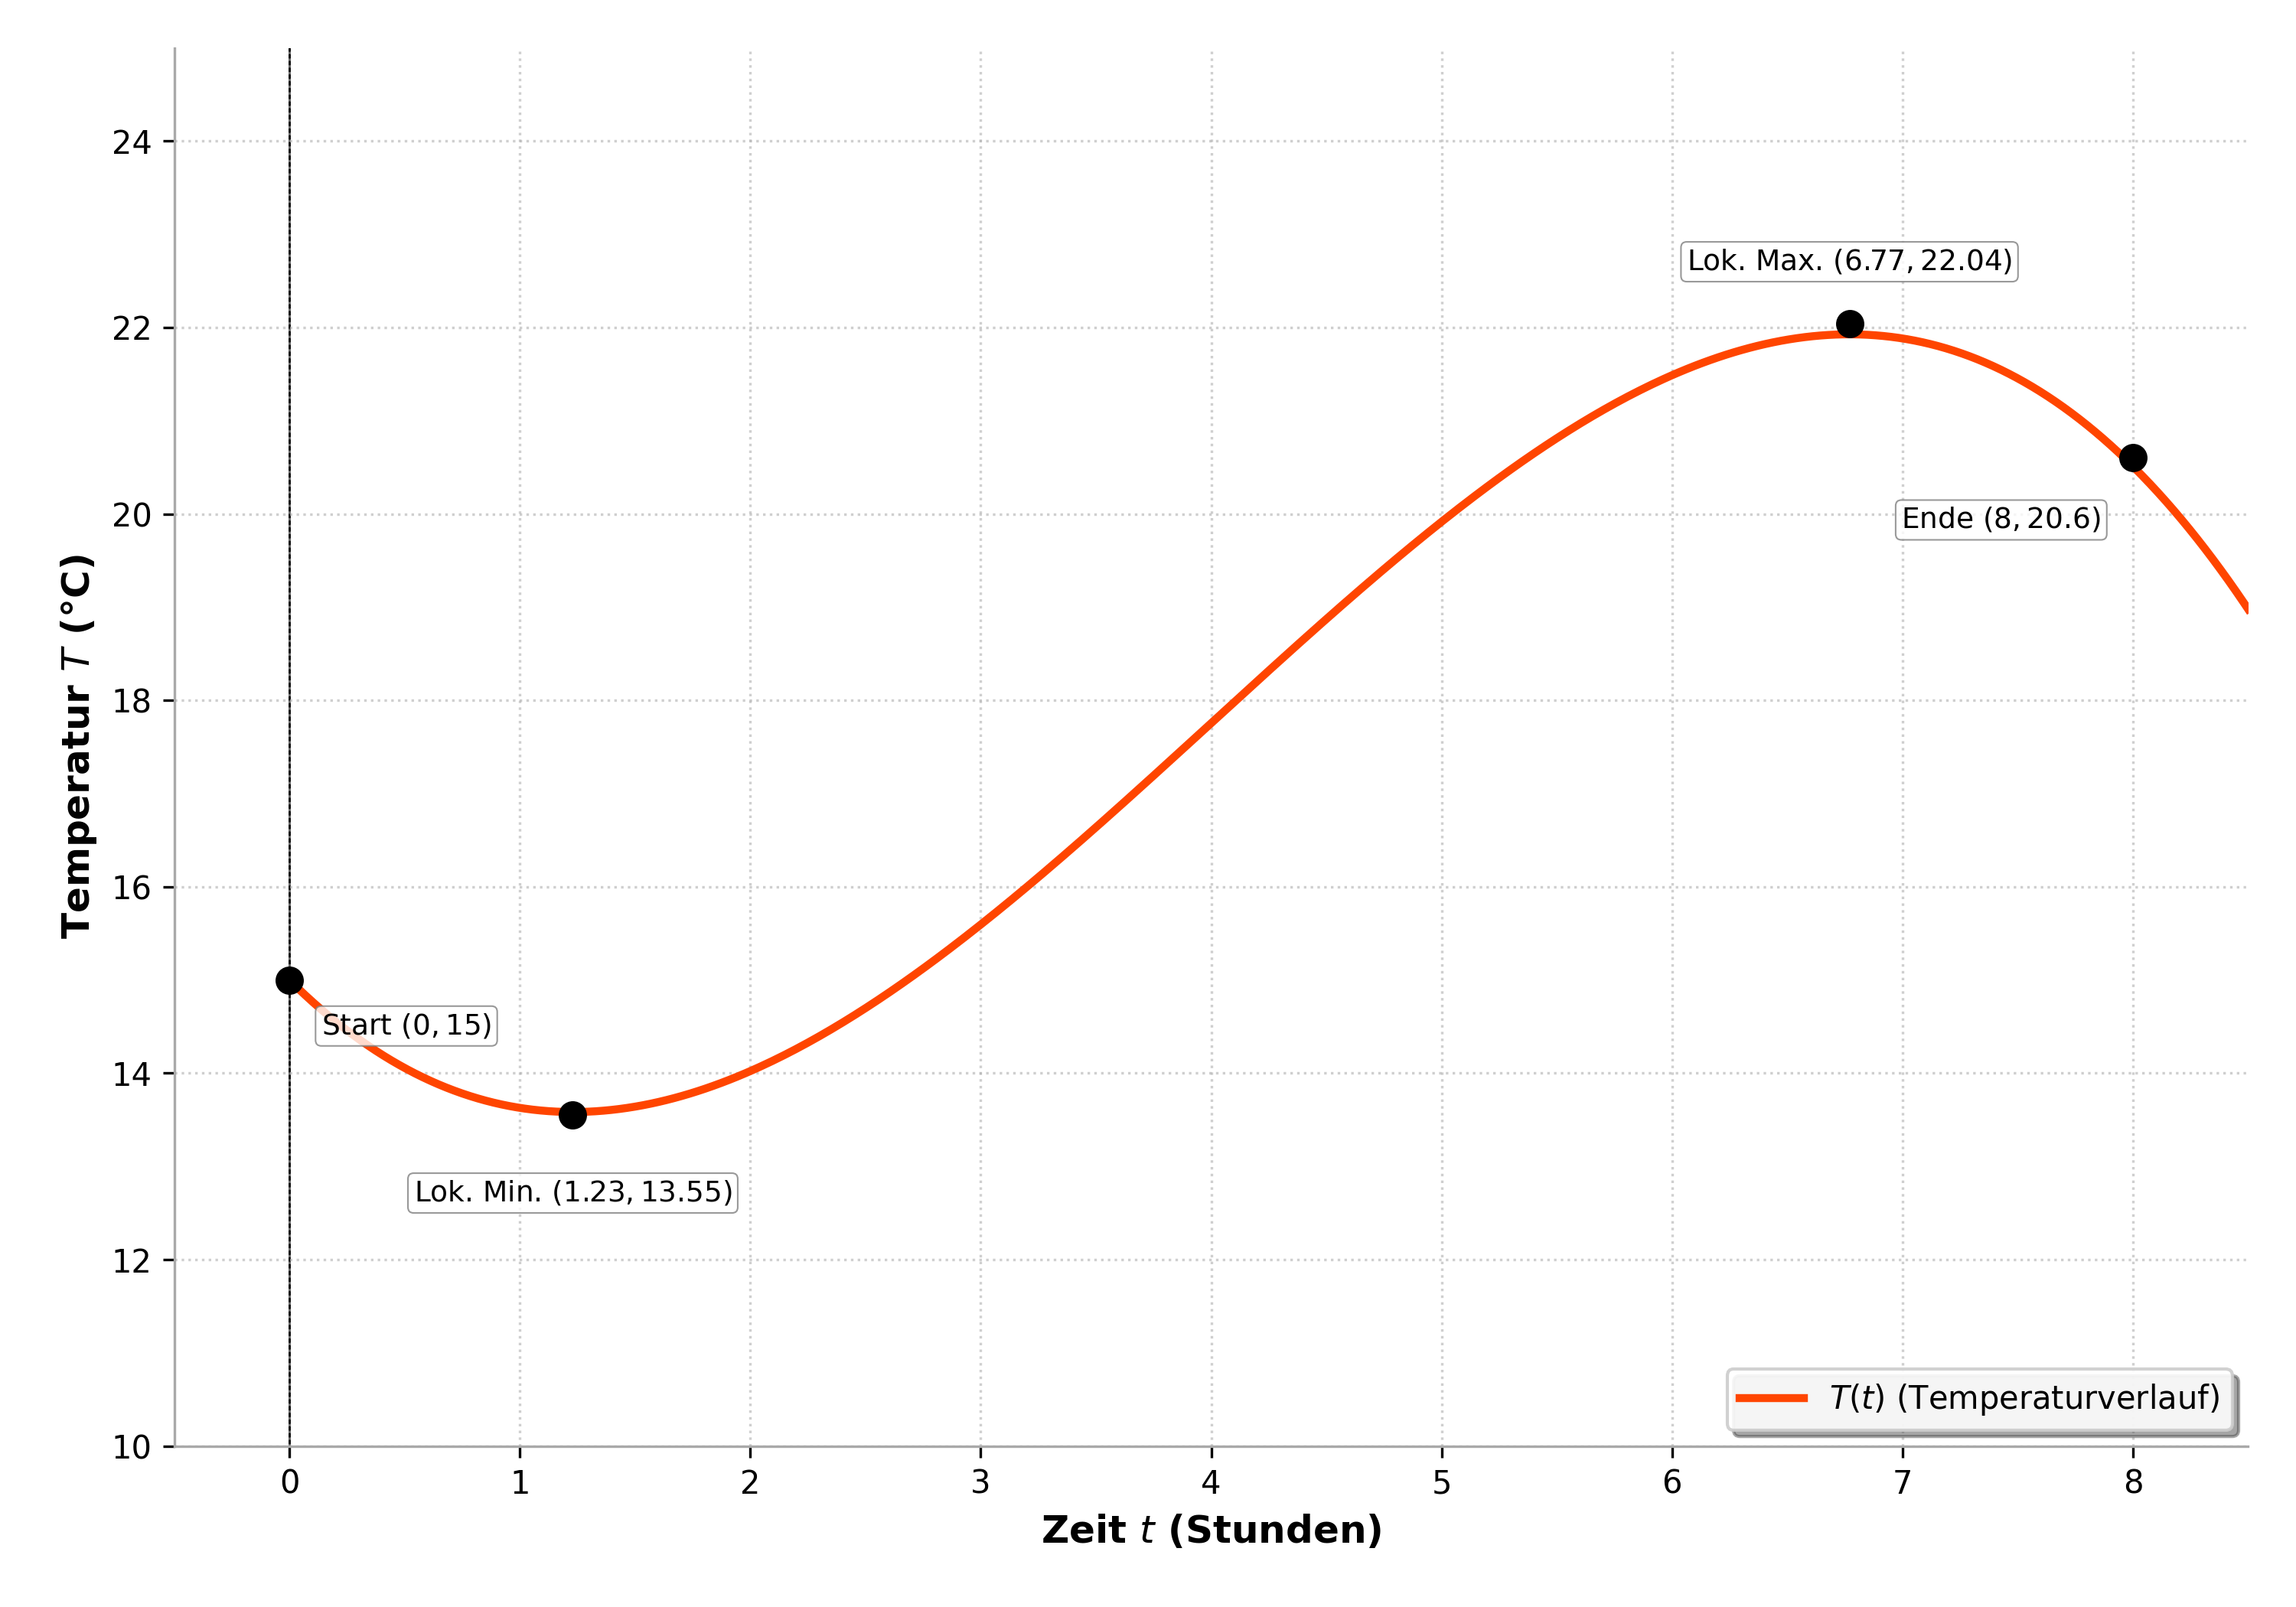
\includegraphics[width=0.8\textwidth]{grafiken/temperaturverlauf_graph.png}
        % --- Beschreibung der Grafik für T(t) ---
        % Die Grafik zeigt ein Koordinatensystem. t-Achse von 0 bis 8 (Stunden), T-Achse von ca. 10 bis 25 (Grad Celsius).
        % Der Graph startet bei (0|15). Fällt zu einem lokalen Minimum bei ca. (1.23|13.55).
        % Steigt zu einem lokalen Maximum bei ca. (6.77|22.04).
        % Fällt dann zum Endpunkt (8|20.6).
        % Die Kurve ist glatt und repräsentiert ein Polynom 3. Grades.
        \captionof{figure}{Skizze des Temperaturverlaufs $T(t)$.}
        \label{fig:temperaturverlauf}
        \end{center}
    \end{itemize}
\end{enumerate}

\end{loesungsumgebung}

\begin{aufgabenumgebung}{Extrempunkte finden – Vielfältige Herausforderungen}
Bestimme die lokalen Extrempunkte (Art und Koordinaten) der folgenden Funktionen. Verwende primär das \textbf{Vorzeichenwechselkriterium der ersten Ableitung ($f'(x)$)}. Du kannst deine Ergebnisse zusätzlich mit dem Kriterium der zweiten Ableitung ($f''(x)$) überprüfen, wo dies sinnvoll und einfach möglich ist.
\begin{enumerate}
    \item $f_1(x) = x^3 - 6x^2 + 9x + 1$


    \item $f_2(x) = \frac{1}{4}x^4 - x^3 - 2x^2 + 5$
        % \begin{tippumgebung}{Polynom 4. Grades}
        % Die erste Ableitung $f_2'(x)$ wird ein Polynom 3. Grades sein. Versuche, $x$ auszuklammern, um eine Nullstelle direkt zu finden. Die verbleibende quadratische Gleichung kannst du dann mit der p-q-Formel oder Mitternachtsformel lösen, um weitere Kandidaten für Extremstellen zu erhalten. Diese Funktion kann mehrere Extrempunkte haben.
        % \end{tippumgebung}

    \item $f_3(x) = x^4 - \frac{8}{3}x^3 + 2x^2$
        % \begin{tippumgebung}{Besonderer Fall bei $f_3''(x_E)=0$?}
        % Es kann vorkommen, dass für eine kritische Stelle $x_E$ (also $f_3'(x_E)=0$) auch die zweite Ableitung $f_3''(x_E)=0$ ist. In diesem Fall liefert das Kriterium mit der zweiten Ableitung keine Aussage über die Art des Extrempunkts. Dann musst du auf das Vorzeichenwechselkriterium der ersten Ableitung $f_3'(x)$ zurückgreifen, um zu entscheiden, ob ein Hochpunkt, Tiefpunkt oder vielleicht ein Sattelpunkt (kein Extremum) vorliegt.
        % \end{tippumgebung}

    \item \textbf{Schwer: Funktion mit Parameter $k$} \\
        Gegeben ist die Funktion $f_k(x) = x^3 - 3kx + 2$, wobei $k \in \mathbb{R}$ ein Parameter ist. Untersuche in Abhängigkeit von $k$:
        \begin{itemize}
            \item Für welche Werte von $k$ hat die Funktion $f_k(x)$ keine lokalen Extrempunkte?
            \item Für welche Werte von $k$ hat die Funktion $f_k(x)$ genau einen lokalen Extrempunkt? (Überlege, was das für die Ableitung bedeutet – kann ein Polynom 3. Grades nur einen Extrempunkt haben, wenn es nicht konstant ist?) Was liegt stattdessen an der kritischen Stelle vor, wenn es kein Extremum ist?
            \item Für welche Werte von $k$ hat die Funktion $f_k(x)$ genau zwei lokale Extrempunkte? Bestimme deren Art (Hoch-/Tiefpunkt) und ihre Lage (x-Koordinaten) in Abhängigkeit von $k$.
        \end{itemize}

    \item \textbf{Anwendung: Optimale Form}
        Ein oben offener quaderförmiger Behälter mit quadratischer Grundfläche soll ein Volumen von $V=32 \text{ cm}^3$ haben. Bestimme die Abmessungen (Seitenlänge der Grundfläche und Höhe), für die der Materialverbrauch (also die Oberfläche) minimal wird.
        \begin{enumerate}[label=(\alph*)]
            \item Sei $a$ die Seitenlänge der quadratischen Grundfläche und $h$ die Höhe des Quaders. Stelle die Formel für das Volumen $V$ und die Oberfläche $O$ (Grundfläche + 4 Seitenflächen) auf.
            \item Drücke $h$ mithilfe der Volumenformel durch $a$ aus (Nebenbedingung).
            \item Setze $h$ in die Oberflächenformel ein, um eine Zielfunktion $O(a)$ zu erhalten, die nur noch von $a$ abhängt.
            \item Bestimme die erste Ableitung $O'(a)$ und finde die kritischen Stellen.
            \item Überprüfe mit der zweiten Ableitung $O''(a)$, ob ein Minimum vorliegt. (Hier ist die zweite Ableitung oft der schnellste Weg zur Klassifizierung in Optimierungsaufgaben).
            \item Berechne die optimale Seitenlänge $a$ und die zugehörige Höhe $h$.
        \end{enumerate}
\end{enumerate}
\end{aufgabenumgebung}


\begin{loesungsumgebung}[loes:extrempunkte-vielfaeltig]{Extrempunkte finden – Vielfältige Herausforderungen}
Wir bestimmen die lokalen Extrempunkte der gegebenen Funktionen.

\begin{enumerate}[label=(\alph*)]
    \item \textbf{Funktion $f_1(x) = x^3 - 6x^2 + 9x + 1$}
    \begin{itemize}
        \item \textbf{Erste Ableitung:} $f_1'(x) = 3x^2 - 12x + 9$.
        \item \textbf{Notwendige Bedingung ($f_1'(x)=0$):}
        $3x^2 - 12x + 9 = 0 \quad | :3$
        $x^2 - 4x + 3 = 0$.
        Mit p-q-Formel oder Vieta: $(x-1)(x-3)=0$.
        Kandidaten für Extremstellen: $x_E_1 = 1$, $x_E_2 = 3$.
        \item \textbf{Vorzeichenwechselkriterium von $f_1'(x)$:}
        $f_1'(x) = 3(x-1)(x-3)$ ist eine nach oben geöffnete Parabel.
        \begin{itemize}
            \item Für $x < 1$ (z.B. $x=0$): $f_1'(0) = 9 > 0$ ($f_1$ steigt).
            \item Für $1 < x < 3$ (z.B. $x=2$): $f_1'(2) = 3(4)-12(2)+9 = 12-24+9 = -3 < 0$ ($f_1$ fällt).
            \item Für $x > 3$ (z.B. $x=4$): $f_1'(4) = 3(16)-12(4)+9 = 48-48+9 = 9 > 0$ ($f_1$ steigt).
        \end{itemize}
        \item \textbf{Art und Koordinaten der Extrempunkte:}
        \begin{itemize}
            \item Bei $x_E_1 = 1$: Vorzeichenwechsel von $f_1'(x)$ von $+$ nach $- \Rightarrow$ \textbf{Lokaler Hochpunkt}.
            $y_E_1 = f_1(1) = 1^3 - 6(1)^2 + 9(1) + 1 = 1-6+9+1 = 5$.
            $\rightarrow HP(1|5)$.
            \item Bei $x_E_2 = 3$: Vorzeichenwechsel von $f_1'(x)$ von $-$ nach $+ \Rightarrow$ \textbf{Lokaler Tiefpunkt}.
            $y_E_2 = f_1(3) = 3^3 - 6(3)^2 + 9(3) + 1 = 27 - 54 + 27 + 1 = 1$.
            $\rightarrow TP(3|1)$.
        \end{itemize}
        \item \textbf{Überprüfung mit $f_1''(x)$:}
        $f_1''(x) = 6x - 12$.
        $f_1''(1) = 6(1)-12 = -6 < 0 \Rightarrow$ Hochpunkt.
        $f_1''(3) = 6(3)-12 = 18-12 = 6 > 0 \Rightarrow$ Tiefpunkt. (Bestätigt)
    \end{itemize}

    \item \textbf{Funktion $f_2(x) = \frac{1}{4}x^4 - x^3 - 2x^2 + 5$}
    \begin{itemize}
        \item \textbf{Erste Ableitung:} $f_2'(x) = x^3 - 3x^2 - 4x$.
        \item \textbf{Notwendige Bedingung ($f_2'(x)=0$):}
        $x^3 - 3x^2 - 4x = 0 \Rightarrow x(x^2 - 3x - 4) = 0$.
        $x_E_1 = 0$.
        Für $x^2 - 3x - 4 = 0$: $(x-4)(x+1)=0 \Rightarrow x_E_2 = 4$, $x_E_3 = -1$.
        Kandidaten: $x=-1, 0, 4$.
        \item \textbf{Vorzeichenwechselkriterium von $f_2'(x) = x(x+1)(x-4)$:}
        \begin{itemize}
            \item Intervall $(-\infty, -1)$ (z.B. $x=-2$): $f_2'(-2) = (-2)(-1)(-6) = -12 < 0$.
            \item Intervall $(-1, 0)$ (z.B. $x=-0.5$): $f_2'(-0.5) = (-0.5)(0.5)(-4.5) = 1.125 > 0$.
            \item Intervall $(0, 4)$ (z.B. $x=1$): $f_2'(1) = (1)(2)(-3) = -6 < 0$.
            \item Intervall $(4, \infty)$ (z.B. $x=5$): $f_2'(5) = (5)(6)(1) = 30 > 0$.
        \end{itemize}
        \item \textbf{Art und Koordinaten der Extrempunkte:}
        \begin{itemize}
            \item Bei $x_E_3 = -1$: VZW von $-$ nach $+ \Rightarrow$ \textbf{Lokaler Tiefpunkt}.
            $f_2(-1) = \frac{1}{4}(1) - (-1) - 2(1) + 5 = \frac{1}{4} + 1 - 2 + 5 = 4.25 = \frac{17}{4}$.
            $\rightarrow TP(-1|4.25)$.
            \item Bei $x_E_1 = 0$: VZW von $+$ nach $- \Rightarrow$ \textbf{Lokaler Hochpunkt}.
            $f_2(0) = 5$.
            $\rightarrow HP(0|5)$.
            \item Bei $x_E_2 = 4$: VZW von $-$ nach $+ \Rightarrow$ \textbf{Lokaler Tiefpunkt}.
            $f_2(4) = \frac{1}{4}(256) - 64 - 2(16) + 5 = 64 - 64 - 32 + 5 = -27$.
            $\rightarrow TP(4|-27)$.
        \end{itemize}
        \item \textbf{Überprüfung mit $f_2''(x)$:}
        $f_2''(x) = 3x^2 - 6x - 4$.
        $f_2''(-1) = 3(1) - 6(-1) - 4 = 3+6-4 = 5 > 0 \Rightarrow$ Tiefpunkt.
        $f_2''(0) = -4 < 0 \Rightarrow$ Hochpunkt.
        $f_2''(4) = 3(16) - 6(4) - 4 = 48 - 24 - 4 = 20 > 0 \Rightarrow$ Tiefpunkt. (Bestätigt)
    \end{itemize}

    \item \textbf{Funktion $f_3(x) = x^4 - \frac{8}{3}x^3 + 2x^2$}
    \begin{itemize}
        \item \textbf{Erste Ableitung:} $f_3'(x) = 4x^3 - 8x^2 + 4x$.
        \item \textbf{Notwendige Bedingung ($f_3'(x)=0$):}
        $4x^3 - 8x^2 + 4x = 0 \Rightarrow 4x(x^2 - 2x + 1) = 0 \Rightarrow 4x(x-1)^2 = 0$.
        Kandidaten: $x_E_1 = 0$, $x_E_2 = 1$.
        \item \textbf{Vorzeichenwechselkriterium von $f_3'(x) = 4x(x-1)^2$:}
        Der Faktor $(x-1)^2$ ist immer $\ge 0$. Das Vorzeichen von $f_3'(x)$ (außer bei $x=1$) wird also durch $4x$ bestimmt.
        \begin{itemize}
            \item Für $x < 0$ (z.B. $x=-1$): $f_3'(-1) = 4(-1)(-1-1)^2 = -4(4) = -16 < 0$.
            \item Für $0 < x < 1$ (z.B. $x=0.5$): $f_3'(0.5) = 4(0.5)(0.5-1)^2 = 2(-0.5)^2 = 2(0.25) = 0.5 > 0$.
            \item Für $x > 1$ (z.B. $x=2$): $f_3'(2) = 4(2)(2-1)^2 = 8(1)^2 = 8 > 0$.
        \end{itemize}
        \item \textbf{Art und Koordinaten der Extrempunkte:}
        \begin{itemize}
            \item Bei $x_E_1 = 0$: VZW von $-$ nach $+ \Rightarrow$ \textbf{Lokaler Tiefpunkt}.
            $f_3(0) = 0$.
            $\rightarrow TP(0|0)$.
            \item Bei $x_E_2 = 1$: Kein VZW (von $+$ nach $+$) $\Rightarrow$ \textbf{Sattelpunkt (Terrassenpunkt)}, kein Extremum.
            $f_3(1) = 1 - \frac{8}{3} + 2 = 3 - \frac{8}{3} = \frac{9-8}{3} = \frac{1}{3}$.
            $\rightarrow SP(1|\frac{1}{3})$.
        \end{itemize}
        \item \textbf{Überprüfung mit $f_3''(x)$:}
        $f_3''(x) = 12x^2 - 16x + 4$.
        $f_3''(0) = 4 > 0 \Rightarrow$ Tiefpunkt.
        $f_3''(1) = 12(1)^2 - 16(1) + 4 = 12 - 16 + 4 = 0$. Das Kriterium mit $f_3''(x)$ liefert hier keine Aussage für $x=1$, wie im Tipp erwähnt. Das Vorzeichenwechselkriterium von $f_3'(x)$ hat bereits gezeigt, dass es sich um einen Sattelpunkt handelt.
    \end{itemize}

    \item \textbf{Schwer: Funktion mit Parameter $k$: $f_k(x) = x^3 - 3kx + 2$}
    \begin{itemize}
        \item \textbf{Erste Ableitung:} $f_k'(x) = 3x^2 - 3k$.
        \item \textbf{Notwendige Bedingung ($f_k'(x)=0$):}
        $3x^2 - 3k = 0 \Rightarrow 3x^2 = 3k \Rightarrow x^2 = k$.
        \item \textbf{Fallunterscheidung basierend auf $k$ für $x^2=k$:}
        \begin{itemize}
            \item \textbf{Fall 1: $k < 0$} \\
            Die Gleichung $x^2=k$ hat keine reellen Lösungen, da $x^2 \ge 0$.
            $f_k'(x) = 3x^2 - 3k = 3x^2 + 3|k|$. Da $3x^2 \ge 0$ und $3|k| > 0$ (wenn $k \neq 0$), ist $f_k'(x) > 0$ für alle $x$.
            Die Funktion $f_k(x)$ ist streng monoton steigend und hat \textbf{keine lokalen Extrempunkte}.
            \item \textbf{Fall 2: $k = 0$} \\
            Die Gleichung $x^2=0$ hat die einzige Lösung $x_E=0$.
            $f_0'(x) = 3x^2$.
            Für $x<0$ ist $f_0'(x) > 0$. Für $x>0$ ist $f_0'(x) > 0$.
            Es gibt keinen Vorzeichenwechsel bei $x=0$. $f_0(x)$ hat bei $x=0$ einen \textbf{Sattelpunkt}, aber \textbf{keinen lokalen Extrempunkt}.
            \item \textbf{Fall 3: $k > 0$} \\
            Die Gleichung $x^2=k$ hat zwei verschiedene reelle Lösungen: $x_E_1 = -\sqrt{k}$ und $x_E_2 = \sqrt{k}$.
            $f_k'(x) = 3x^2 - 3k = 3(x^2-k)$. Dies ist eine nach oben geöffnete Parabel mit Nullstellen bei $\pm\sqrt{k}$.
            \begin{itemize}
                \item Für $x < -\sqrt{k}$: $f_k'(x) > 0$.
                \item Für $-\sqrt{k} < x < \sqrt{k}$: $f_k'(x) < 0$.
                \item Für $x > \sqrt{k}$: $f_k'(x) > 0$.
            \end{itemize}
            Bei $x_E_1 = -\sqrt{k}$: VZW von $+$ nach $- \Rightarrow$ \textbf{Lokaler Hochpunkt}.
            Bei $x_E_2 = \sqrt{k}$: VZW von $-$ nach $+ \Rightarrow$ \textbf{Lokaler Tiefpunkt}.
            Die Funktion $f_k(x)$ hat \textbf{genau zwei lokale Extrempunkte}.
        \end{itemize}
        \item \textbf{Antworten auf die Fragen:}
        \begin{itemize}
            \item Keine lokalen Extrempunkte: Für $k \le 0$.
            \item Genau einen lokalen Extrempunkt: Ein Polynom 3. Grades hat entweder zwei lokale Extrema oder keinen (im Fall eines Sattelpunkts). Es gibt also keinen Fall mit genau einem lokalen Extremum (Hoch- oder Tiefpunkt). Für $k=0$ gibt es einen Sattelpunkt, was kein Extremum ist.
            \item Genau zwei lokale Extrempunkte: Für $k > 0$.
            Lage: $x_{HP} = -\sqrt{k}$ (Hochpunkt), $x_{TP} = \sqrt{k}$ (Tiefpunkt).
        \end{itemize}
    \end{itemize}

    \item \textbf{Anwendung: Optimale Form eines Behälters}
    Gegeben: Oben offener Quader, quadratische Grundfläche $a \cdot a$, Höhe $h$, Volumen $V=32 \text{ cm}^3$. Gesucht: Minimale Oberfläche $O$.
    \begin{enumerate}[label=(\roman*)]
        \item \textbf{Formeln für Volumen $V$ und Oberfläche $O$:}
        $V = a^2 h$
        $O = \text{Grundfläche} + \text{Mantelfläche} = a^2 + 4ah$
        \item \textbf{$h$ durch $a$ ausdrücken (Nebenbedingung):}
        Aus $V=32$: $a^2h = 32 \Rightarrow h = \frac{32}{a^2}$ (gültig für $a>0$).
        \item \textbf{Zielfunktion $O(a)$:}
        $h$ in $O$ einsetzen:
        $O(a) = a^2 + 4a \left(\frac{32}{a^2}\right) = a^2 + \frac{128}{a} = a^2 + 128a^{-1}$.
        \item \textbf{Erste Ableitung $O'(a)$ und kritische Stellen:}
        $O'(a) = \frac{d}{da}(a^2 + 128a^{-1}) = 2a - 128a^{-2} = 2a - \frac{128}{a^2}$.
        Setze $O'(a)=0$ für kritische Stellen:
        $2a - \frac{128}{a^2} = 0 \quad | \cdot a^2 \quad (a \neq 0)$
        $2a^3 - 128 = 0$
        $$
        \begin{array}{r c l c l}
        \umformung{2a^3 - 128}{0}{+}{128}
        \umformung{2a^3}{128}{\div}{2}
        \umformung{a^3}{64}{\text{dritte Wurzel ziehen}}{}
        \umformungend{a}{4}
        \end{array}
        $$
        Die einzige positive kritische Stelle ist $a=4\,$cm.
        \item \textbf{Überprüfung mit der zweiten Ableitung $O''(a)$:}
        $O''(a) = \frac{d}{da}(2a - 128a^{-2}) = 2 - 128(-2)a^{-3} = 2 + 256a^{-3} = 2 + \frac{256}{a^3}$.
        Für $a=4$: $O''(4) = 2 + \frac{256}{4^3} = 2 + \frac{256}{64} = 2 + 4 = 6$.
        Da $O''(4) = 6 > 0$, liegt bei $a=4$ ein lokales Minimum für die Oberfläche vor.
        \item \textbf{Optimale Seitenlänge $a$ und Höhe $h$:}
        Die optimale Seitenlänge der Grundfläche ist $a = 4\,$cm.
        Die zugehörige Höhe ist $h = \frac{32}{a^2} = \frac{32}{4^2} = \frac{32}{16} = 2\,$cm.
        Die Abmessungen für den minimalen Materialverbrauch sind $4\,$cm $\cdot$ $4\,$cm für die Grundfläche und $2\,$cm für die Höhe.
    \end{enumerate}
\end{enumerate}

\end{loesungsumgebung}

\begin{aufgabenumgebung}{Höhere Ableitungen berechnen}
Bestimme die erste, zweite und dritte Ableitung der folgenden Funktionen:
\begin{enumerate}
    \item $f(x) = 2x^3 - 9x^2 + 12x - 5$
    \item $g(x) = -0.1x^5 + x^3 - 7$
    \item $h(t) = 2t^2 - \frac{1}{t}$ (Tipp: $\frac{1}{t} = t^{-1}$)
\end{enumerate}
\end{aufgabenumgebung}

\begin{loesungsumgebung}[loes:hoehere-ableitungen]{Höhere Ableitungen berechnen}
Wir bestimmen die erste ($f'(x)$), zweite ($f''(x)$) und dritte ($f'''(x)$) Ableitung der gegebenen Funktionen.

\begin{enumerate}[label=(\alph*)]
    \item \textbf{Funktion $f(x) = 2x^3 - 9x^2 + 12x - 5$}
    \begin{itemize}
        \item \textbf{Erste Ableitung $f'(x)$:}
        $$ f'(x) = \frac{d}{dx}(2x^3 - 9x^2 + 12x - 5) $$
        $$ f'(x) = 2 \cdot 3x^{3-1} - 9 \cdot 2x^{2-1} + 12 \cdot 1x^{1-1} - 0 $$
        $$ f'(x) = 6x^2 - 18x + 12 $$
        \item \textbf{Zweite Ableitung $f''(x)$:}
        $$ f''(x) = \frac{d}{dx}(6x^2 - 18x + 12) $$
        $$ f''(x) = 6 \cdot 2x^{2-1} - 18 \cdot 1x^{1-1} + 0 $$
        $$ f''(x) = 12x - 18 $$
        \item \textbf{Dritte Ableitung $f'''(x)$:}
        $$ f'''(x) = \frac{d}{dx}(12x - 18) $$
        $$ f'''(x) = 12 \cdot 1x^{1-1} - 0 $$
        $$ f'''(x) = 12 $$
    \end{itemize}

    \item \textbf{Funktion $g(x) = -0.1x^5 + x^3 - 7$}
    \begin{itemize}
        \item \textbf{Erste Ableitung $g'(x)$:}
        $$ g'(x) = \frac{d}{dx}(-0.1x^5 + x^3 - 7) $$
        $$ g'(x) = -0.1 \cdot 5x^{5-1} + 3x^{3-1} - 0 $$
        $$ g'(x) = -0.5x^4 + 3x^2 $$
        \item \textbf{Zweite Ableitung $g''(x)$:}
        $$ g''(x) = \frac{d}{dx}(-0.5x^4 + 3x^2) $$
        $$ g''(x) = -0.5 \cdot 4x^{4-1} + 3 \cdot 2x^{2-1} $$
        $$ g''(x) = -2x^3 + 6x $$
        \item \textbf{Dritte Ableitung $g'''(x)$:}
        $$ g'''(x) = \frac{d}{dx}(-2x^3 + 6x) $$
        $$ g'''(x) = -2 \cdot 3x^{3-1} + 6 \cdot 1x^{1-1} $$
        $$ g'''(x) = -6x^2 + 6 $$
    \end{itemize}

    \item \textbf{Funktion $h(t) = 2t^2 - \frac{1}{t}$} \\
    Zuerst schreiben wir die Funktion mit Potenzschreibweise um: $h(t) = 2t^2 - t^{-1}$.
    \begin{itemize}
        \item \textbf{Erste Ableitung $h'(t)$:}
        $$ h'(t) = \frac{d}{dt}(2t^2 - t^{-1}) $$
        $$ h'(t) = 2 \cdot 2t^{2-1} - (-1)t^{-1-1} $$
        $$ h'(t) = 4t + t^{-2} = 4t + \frac{1}{t^2} $$
        \item \textbf{Zweite Ableitung $h''(t)$:}
        $$ h''(t) = \frac{d}{dt}(4t + t^{-2}) $$
        $$ h''(t) = 4 \cdot 1t^{1-1} + (-2)t^{-2-1} $$
        $$ h''(t) = 4 - 2t^{-3} = 4 - \frac{2}{t^3} $$
        \item \textbf{Dritte Ableitung $h'''(t)$:}
        $$ h'''(t) = \frac{d}{dt}(4 - 2t^{-3}) $$
        $$ h'''(t) = 0 - 2(-3)t^{-3-1} $$
        $$ h'''(t) = 6t^{-4} = \frac{6}{t^4} $$
    \end{itemize}
\end{enumerate}

\end{loesungsumgebung}

\begin{aufgabenumgebung}{Krümmung und Wendepunkte – Vielfältige Untersuchungen}
Untersuche die folgenden Funktionen auf ihr Krümmungsverhalten (Intervalle für Links- und Rechtskrümmung) und bestimme gegebenenfalls die Koordinaten der Wendepunkte. Nutze dazu die zweite und, falls nötig, die dritte Ableitung.
\begin{enumerate}
    \item $f_1(x) = \frac{1}{12}x^4 - \frac{1}{2}x^3 + x^2 + 1$
    \item $f_2(x) = x^5 - 5x^4 + 3x - 2$


    \item \textbf{Anwendung: Infektionsgeschehen} \\
        Die Funktion $N(t) = -t^3 + 12t^2 + 20t$ beschreibt die Anzahl der neu infizierten Personen pro Tag während einer Grippewelle ($t$ in Tagen, $t \ge 0$).
        \begin{itemize}
            \item Bestimme die Funktion $N'(t)$, welche die Änderungsrate der Neuinfektionen (also die 'Geschwindigkeit' der Ausbreitung) beschreibt.
            \item Bestimme die Funktion $N''(t)$, welche die Änderungsrate der Wachstumsrate der Neuinfektionen beschreibt.
            \item Zu welchem Zeitpunkt $t_W$ ist die Zunahme der täglichen Neuinfektionen am größten? (Das bedeutet, $N'(t)$ hat ein Maximum, also suche einen Wendepunkt von $N(t)$, an dem die Krümmung von links nach rechts wechselt, d.h. $N''(t_W)=0$ und $N'''(t_W)<0$).
            \item Interpretiere die Bedeutung dieses Zeitpunktes $t_W$ für den Verlauf der Grippewelle. Was passiert mit der Zunahme der Neuinfektionen nach diesem Zeitpunkt?
        \end{itemize}

    \item \textbf{Schwer: Funktion mit Parameter $a$} \\
        Gegeben ist die Funktionenschar $f_a(x) = x^4 + ax^3$ mit $a \in \mathbb{R}, a \neq 0$.
        \begin{itemize}
            \item Bestimme die zweite Ableitung $f_a''(x)$.
            \item Zeige, dass $x_1=0$ eine potentielle Wendestelle ist. Untersuche mit der dritten Ableitung $f_a'''(x)$, ob für $x_1=0$ tatsächlich ein Wendepunkt vorliegt.
            \item Bestimme die andere potentielle Wendestelle $x_2$ in Abhängigkeit von $a$.
            \item Für welche Werte von $a$ existiert dieser zweite Wendepunkt $x_2$? (Beachte, dass $x_2 \neq x_1$ sein sollte für einen \textit{anderen} Wendepunkt).
            \item Untersuche das Krümmungsverhalten für $a=2$ und $a=-2$ und skizziere grob die Verläufe (ohne vollständige Kurvendiskussion, Fokus auf Krümmung und Wendepunkte).
        \end{itemize}
\end{enumerate}
\end{aufgabenumgebung}


\begin{loesungsumgebung}[loes:kruemmung-wendepunkte-vielfalt]{Krümmung und Wendepunkte – Vielfältige Untersuchungen}
Wir untersuchen die gegebenen Funktionen auf ihr Krümmungsverhalten und bestimmen die Koordinaten eventueller Wendepunkte.

\begin{enumerate}[label=(\alph*)]
    \item \textbf{Funktion $f_1(x) = \frac{1}{12}x^4 - \frac{1}{2}x^3 + x^2 + 1$}
    \begin{itemize}
        \item \textbf{Erste Ableitung:} $f_1'(x) = \frac{4}{12}x^3 - \frac{3}{2}x^2 + 2x = \frac{1}{3}x^3 - \frac{3}{2}x^2 + 2x$.
        \item \textbf{Zweite Ableitung:} $f_1''(x) = 3 \cdot \frac{1}{3}x^2 - 2 \cdot \frac{3}{2}x + 2 = x^2 - 3x + 2$.
        \item \textbf{Nullstellen der zweiten Ableitung ($f_1''(x)=0$):}
        $x^2 - 3x + 2 = 0$. Mit dem Satz von Vieta (oder p-q-Formel): $(x-1)(x-2)=0$.
        Potentielle Wendestellen sind $x_{W1} = 1$ und $x_{W2} = 2$.
        \item \textbf{Dritte Ableitung:} $f_1'''(x) = 2x - 3$.
        \item \textbf{Überprüfung der potentiellen Wendestellen:}
        \begin{itemize}
            \item Für $x_{W1} = 1$: $f_1'''(1) = 2(1) - 3 = -1 \neq 0$. Also liegt bei $x=1$ ein Wendepunkt vor.
            \item Für $x_{W2} = 2$: $f_1'''(2) = 2(2) - 3 = 1 \neq 0$. Also liegt bei $x=2$ ein Wendepunkt vor.
        \end{itemize}
        \item \textbf{Krümmungsverhalten ($f_1''(x) = x^2 - 3x + 2$ ist eine nach oben geöffnete Parabel):}
        \begin{itemize}
            \item Für $x < 1$: $f_1''(x) > 0 \Rightarrow$ Linkskrümmung (konvex).
            \item Für $1 < x < 2$: $f_1''(x) < 0 \Rightarrow$ Rechtskrümmung (konkav).
            \item Für $x > 2$: $f_1''(x) > 0 \Rightarrow$ Linkskrümmung (konvex).
        \end{itemize}
        \item \textbf{Koordinaten der Wendepunkte:}
        \begin{itemize}
            \item $y_{W1} = f_1(1) = \frac{1}{12}(1)^4 - \frac{1}{2}(1)^3 + (1)^2 + 1 = \frac{1}{12} - \frac{1}{2} + 1 + 1 = \frac{1-6+12+12}{12} = \frac{19}{12}$.
            $\rightarrow WP_1(1|\frac{19}{12})$.
            \item $y_{W2} = f_1(2) = \frac{1}{12}(2)^4 - \frac{1}{2}(2)^3 + (2)^2 + 1 = \frac{16}{12} - \frac{8}{2} + 4 + 1 = \frac{4}{3} - 4 + 4 + 1 = \frac{4}{3} + 1 = \frac{7}{3}$.
            $\rightarrow WP_2(2|\frac{7}{3})$.
        \end{itemize}
    \end{itemize}

    \item \textbf{Funktion $f_2(x) = x^5 - 5x^4 + 3x - 2$}
    \begin{itemize}
        \item \textbf{Erste Ableitung:} $f_2'(x) = 5x^4 - 20x^3 + 3$.
        \item \textbf{Zweite Ableitung:} $f_2''(x) = 20x^3 - 60x^2$.
        \item \textbf{Nullstellen der zweiten Ableitung ($f_2''(x)=0$):}
        $20x^3 - 60x^2 = 0 \Rightarrow 20x^2(x-3) = 0$.
        Potentielle Wendestellen sind $x_{W1} = 0$ und $x_{W2} = 3$.
        \item \textbf{Dritte Ableitung:} $f_2'''(x) = 60x^2 - 120x = 60x(x-2)$.
        \item \textbf{Überprüfung der potentiellen Wendestellen:}
        \begin{itemize}
            \item Für $x_{W1} = 0$: $f_2'''(0) = 60(0)(0-2) = 0$. Hier liefert $f_2'''(x)$ keine Aussage. Wir müssen das Vorzeichen von $f_2''(x)$ untersuchen.
            \item Für $x_{W2} = 3$: $f_2'''(3) = 60(3)(3-2) = 180 \neq 0$. Also liegt bei $x=3$ ein Wendepunkt vor.
        \end{itemize}
        \item \textbf{Krümmungsverhalten ($f_2''(x) = 20x^2(x-3)$):}
        Der Faktor $20x^2$ ist für $x \neq 0$ positiv. Das Vorzeichen von $f_2''(x)$ wird also (für $x \neq 0$) durch $(x-3)$ bestimmt.
        \begin{itemize}
            \item Für $x < 0$: $x-3 < 0 \Rightarrow f_2''(x) < 0 \Rightarrow$ Rechtskrümmung.
            \item Für $0 < x < 3$: $x-3 < 0 \Rightarrow f_2''(x) < 0 \Rightarrow$ Rechtskrümmung.
            \item Für $x > 3$: $x-3 > 0 \Rightarrow f_2''(x) > 0 \Rightarrow$ Linkskrümmung.
        \end{itemize}
        An der Stelle $x=0$ wechselt $f_2''(x)$ das Vorzeichen nicht (es ist $f_2''(x) \le 0$ in der Umgebung von $x=0$). Daher ist bei $x=0$ \textbf{kein Wendepunkt}.
        \item \textbf{Koordinaten des Wendepunkts:}
        \begin{itemize}
            \item $y_{W2} = f_2(3) = (3)^5 - 5(3)^4 + 3(3) - 2 = 243 - 5(81) + 9 - 2 = 243 - 405 + 7 = -155$.
            $\rightarrow WP(3|-155)$.
        \end{itemize}
    \end{itemize}

    \item \textbf{Anwendung: Infektionsgeschehen $N(t) = -t^3 + 12t^2 + 20t$ ($t \ge 0$)}
    \begin{itemize}
        \item \textbf{$N'(t)$ (Änderungsrate der Neuinfektionen):}
        $N'(t) = -3t^2 + 24t + 20$.
        \item \textbf{$N''(t)$ (Änderungsrate der Wachstumsrate):}
        $N''(t) = -6t + 24$.
        \item \textbf{Zeitpunkt $t_W$ der größten Zunahme der Neuinfektionen:}
        Dies ist der Zeitpunkt, an dem $N'(t)$ ein Maximum hat, also $N''(t_W)=0$ und $N'''(t_W)<0$.
        $N''(t_W)=0 \Rightarrow -6t_W + 24 = 0 \Rightarrow 6t_W = 24 \Rightarrow t_W = 4$.
        Die dritte Ableitung ist $N'''(t) = -6$.
        Da $N'''(4) = -6 < 0$, hat $N'(t)$ bei $t_W=4$ ein Maximum. Der Punkt $t_W=4$ ist ein Wendepunkt der Funktion $N(t)$, an dem die Krümmung von einer Linkskrümmung ($N''(t)>0$ für $t<4$) zu einer Rechtskrümmung ($N''(t)<0$ für $t>4$) wechselt.
        Der Zeitpunkt, an dem die Zunahme der täglichen Neuinfektionen am größten ist, ist $t_W = 4$ Tage.
        \item \textbf{Interpretation von $t_W=4$:}
        Am 4. Tag nach Beobachtungsbeginn ist der Anstieg der Zahl der täglichen Neuinfektionen am stärksten. Bis zu diesem Zeitpunkt beschleunigt sich die Ausbreitung der Grippewelle (die Zahl der Neuinfektionen pro Tag steigt immer schneller). Nach dem 4. Tag nehmen die täglichen Neuinfektionen zwar möglicherweise immer noch zu (solange $N'(t)>0$), aber die Geschwindigkeit dieser Zunahme verlangsamt sich. Der Wendepunkt markiert den Übergang von exponentiell anmutendem Wachstum zu einem gebremsten Wachstum der Neuinfektionszahlen pro Tag.
    \end{itemize}

    \item \textbf{Schwer: Funktion mit Parameter $a$: $f_a(x) = x^4 + ax^3$ ($a \in \mathbb{R}, a \neq 0$)}
    \begin{itemize}
        \item \textbf{Zweite Ableitung $f_a''(x)$:}
        $f_a'(x) = 4x^3 + 3ax^2$.
        $f_a''(x) = 12x^2 + 6ax = 6x(2x+a)$.
        \item \textbf{Untersuchung von $x_1=0$ als potentielle Wendestelle:}
        $f_a''(0) = 6(0)(2(0)+a) = 0$. Also ist $x_1=0$ eine potentielle Wendestelle.
        Dritte Ableitung: $f_a'''(x) = 24x + 6a$.
        $f_a'''(0) = 24(0) + 6a = 6a$.
        Da $a \neq 0$ (laut Aufgabenstellung), ist $f_a'''(0) = 6a \neq 0$.
        Somit liegt bei $x_1=0$ tatsächlich ein Wendepunkt vor.
        \item \textbf{Andere potentielle Wendestelle $x_2$:}
        Aus $f_a''(x) = 6x(2x+a)=0$ folgt neben $x_1=0$ auch $2x+a=0$.
        $2x = -a \Rightarrow x_2 = -\frac{a}{2}$.
        \item \textbf{Existenz des zweiten Wendepunkts $x_2$:}
        Der Wendepunkt $x_2 = -\frac{a}{2}$ existiert für alle $a \in \mathbb{R}$.
        Damit es ein \textit{anderer} Wendepunkt als $x_1=0$ ist, muss $x_2 \neq 0$, also $-\frac{a}{2} \neq 0$. Dies ist erfüllt, da $a \neq 0$ vorgegeben ist.
        Also gibt es für alle $a \neq 0$ zwei verschiedene Wendepunkte bei $x=0$ und $x=-a/2$. (Überprüfung für $x_2$: $f_a'''(-a/2) = 24(-a/2) + 6a = -12a + 6a = -6a$. Da $a \neq 0$, ist $f_a'''(-a/2) \neq 0$).
        \item \textbf{Krümmungsverhalten und Skizzen für $a=2$ und $a=-2$:}
        \begin{itemize}
            \item \textbf{Fall $a=2$:} $f_2(x) = x^4 + 2x^3$.
            $f_2''(x) = 12x^2 + 12x = 12x(x+1)$.
            Wendestellen bei $x_{W_1}=0$ und $x_{W_2}=-1$.
            $f_2''(x)$ ist eine nach oben geöffnete Parabel.
            Krümmungsverhalten:
            \begin{itemize}
                \item $(-\infty, -1)$: $f_2''(x) > 0 \Rightarrow$ Linkskrümmung.
                \item $(-1, 0)$: $f_2''(x) < 0 \Rightarrow$ Rechtskrümmung.
                \item $(0, \infty)$: $f_2''(x) > 0 \Rightarrow$ Linkskrümmung.
            \end{itemize}
            \begin{center}
            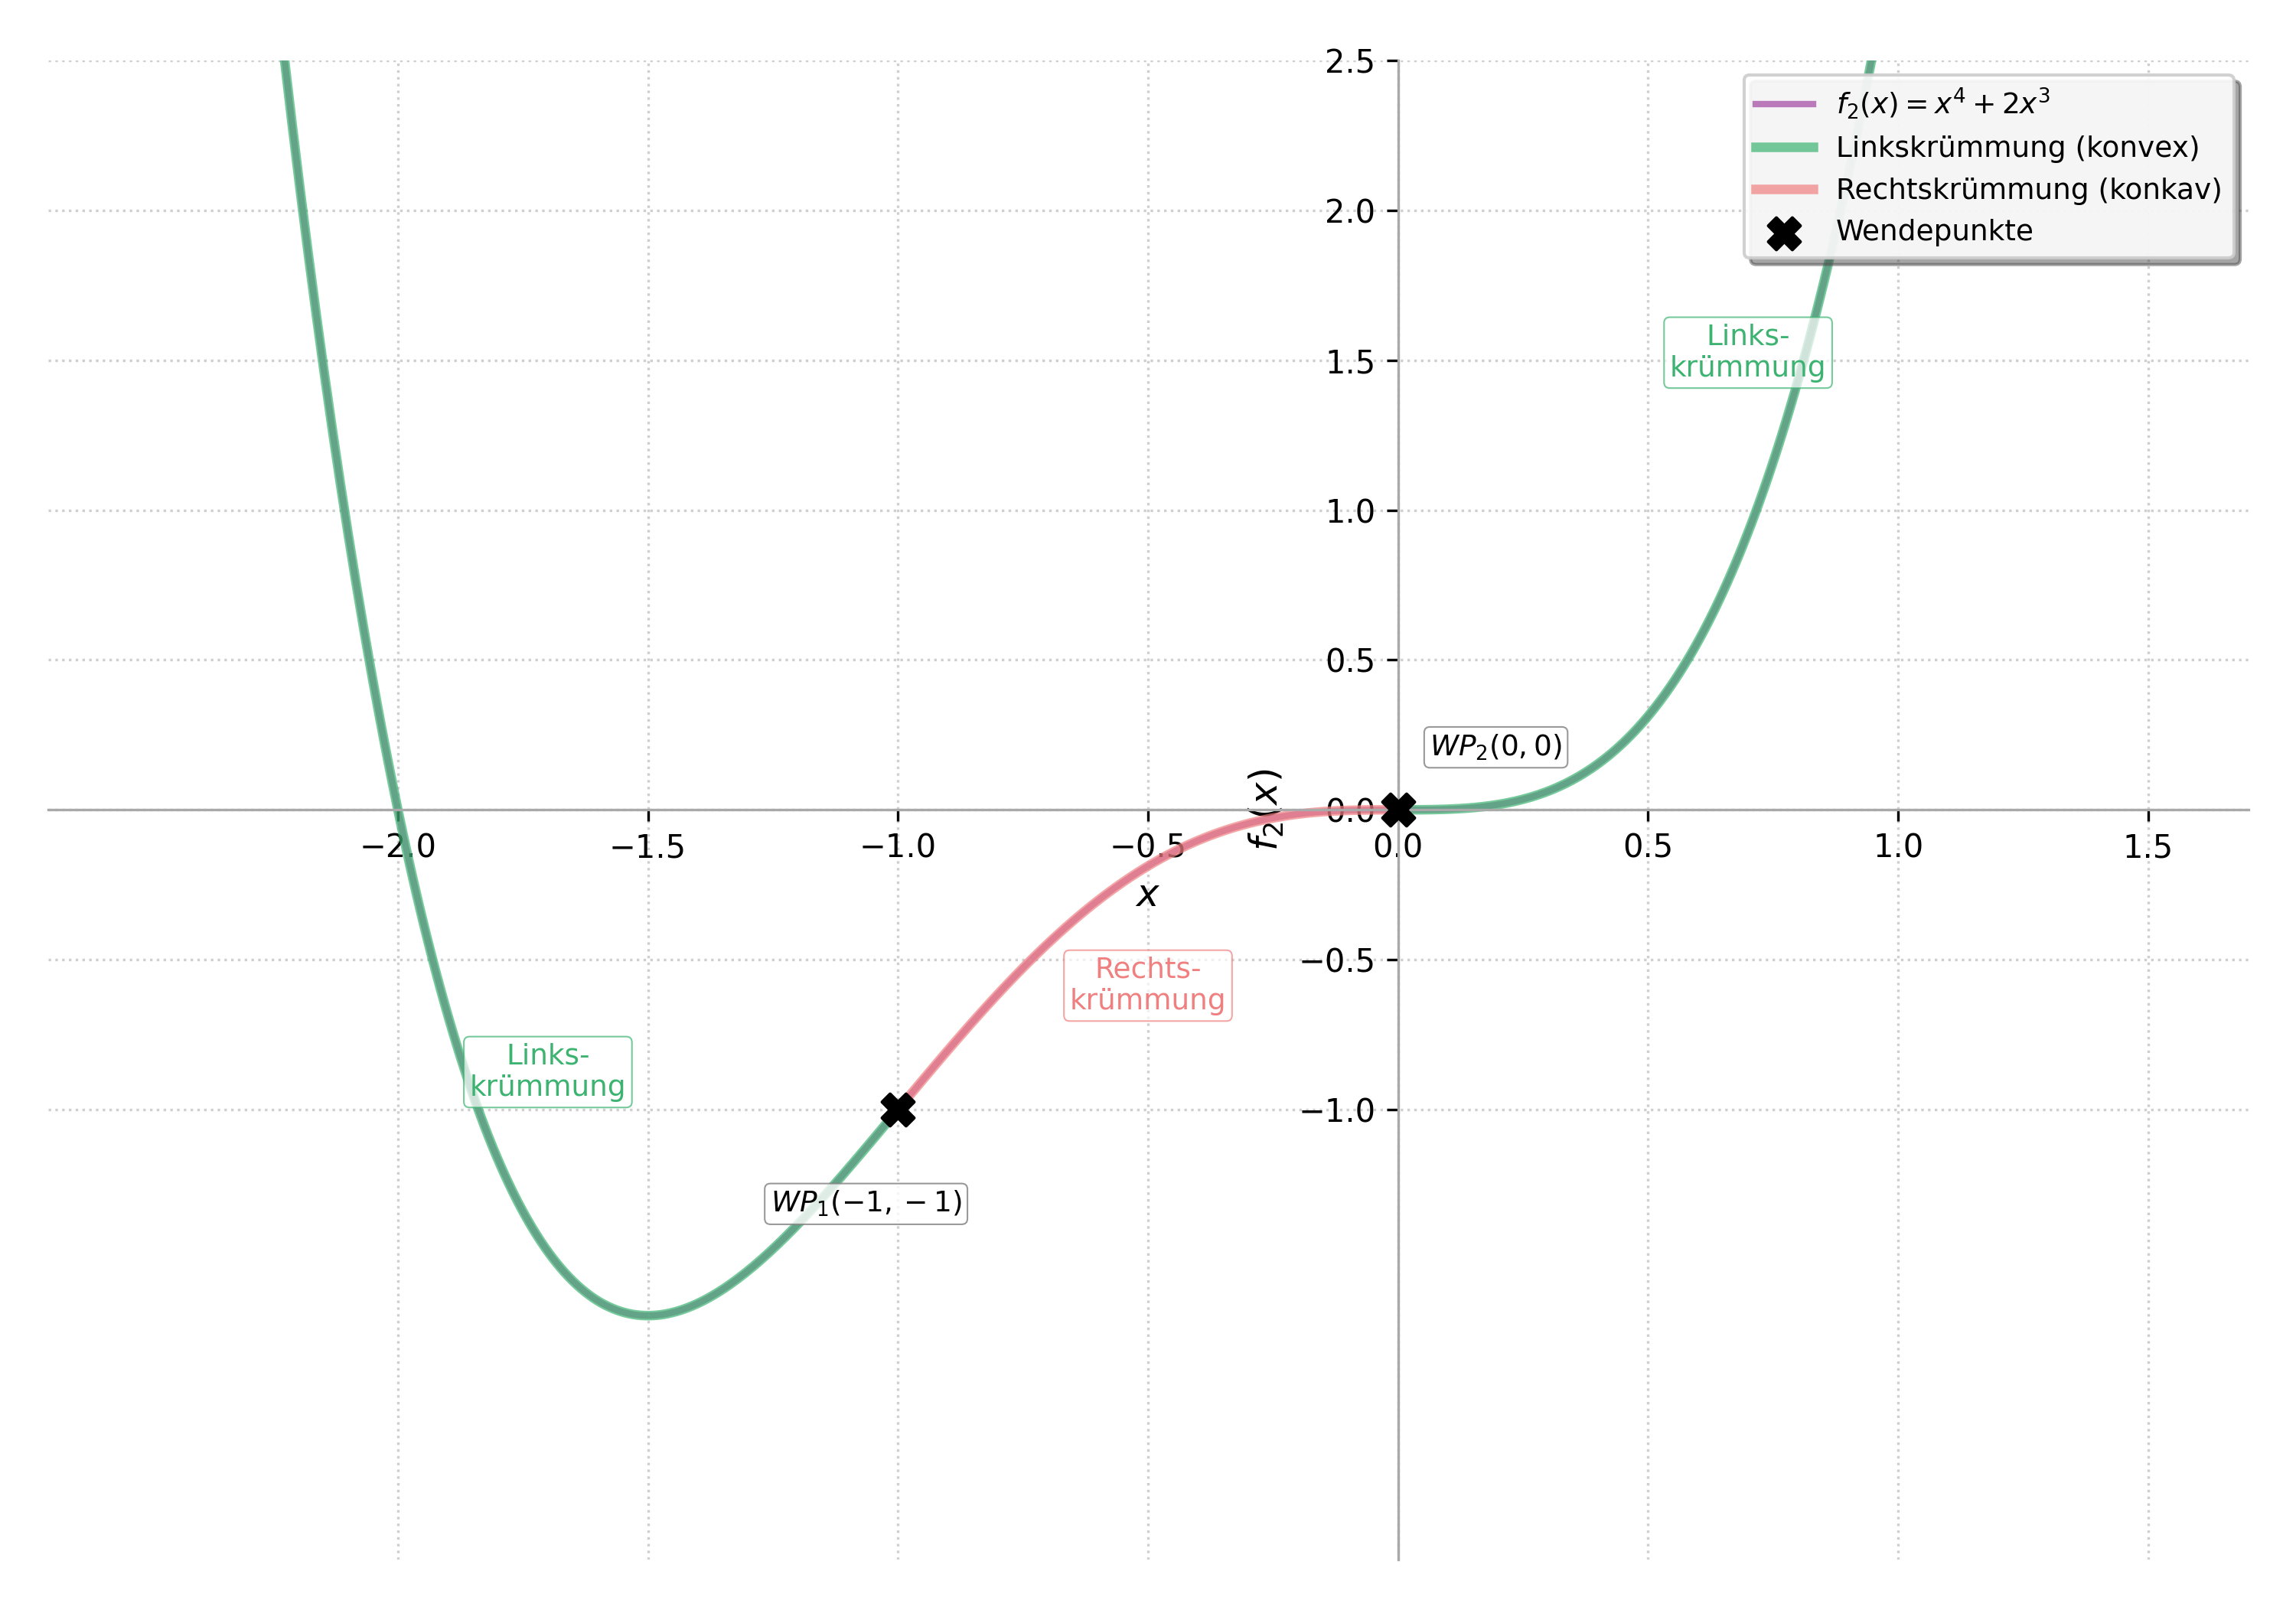
\includegraphics[width=0.8\textwidth]{grafiken/fa_kruemmung_a_pos2.png}
            \captionof{figure}{Grobe Skizze von $f_2(x)=x^4+2x^3$ mit Fokus auf Krümmung (WP bei -1 und 0).}
            \label{fig:fa_kruemmung_a_pos2}
            \end{center}
            \textit{Skizzenbeschreibung:} Der Graph kommt von links oben (Linkskrümmung), hat einen Wendepunkt bei $x=-1$ (Übergang zur Rechtskrümmung), durchläuft einen Bereich mit Rechtskrümmung, hat einen weiteren Wendepunkt bei $x=0$ (Übergang zur Linkskrümmung) und geht dann nach rechts oben weg (Linkskrümmung). Das Globalverhalten ist wie $x^4$.

            \item \textbf{Fall $a=-2$:} $f_{-2}(x) = x^4 - 2x^3$.
            $f_{-2}''(x) = 12x^2 - 12x = 12x(x-1)$.
            Wendestellen bei $x_W_1=0$ und $x_W_2=1$.
            $f_{-2}''(x)$ ist eine nach oben geöffnete Parabel.
            Krümmungsverhalten:
            \begin{itemize}
                \item $(-\infty, 0)$: $f_{-2}''(x) > 0 \Rightarrow$ Linkskrümmung.
                \item $(0, 1)$: $f_{-2}''(x) < 0 \Rightarrow$ Rechtskrümmung.
                \item $(1, \infty)$: $f_{-2}''(x) > 0 \Rightarrow$ Linkskrümmung.
            \end{itemize}
            \begin{center}
            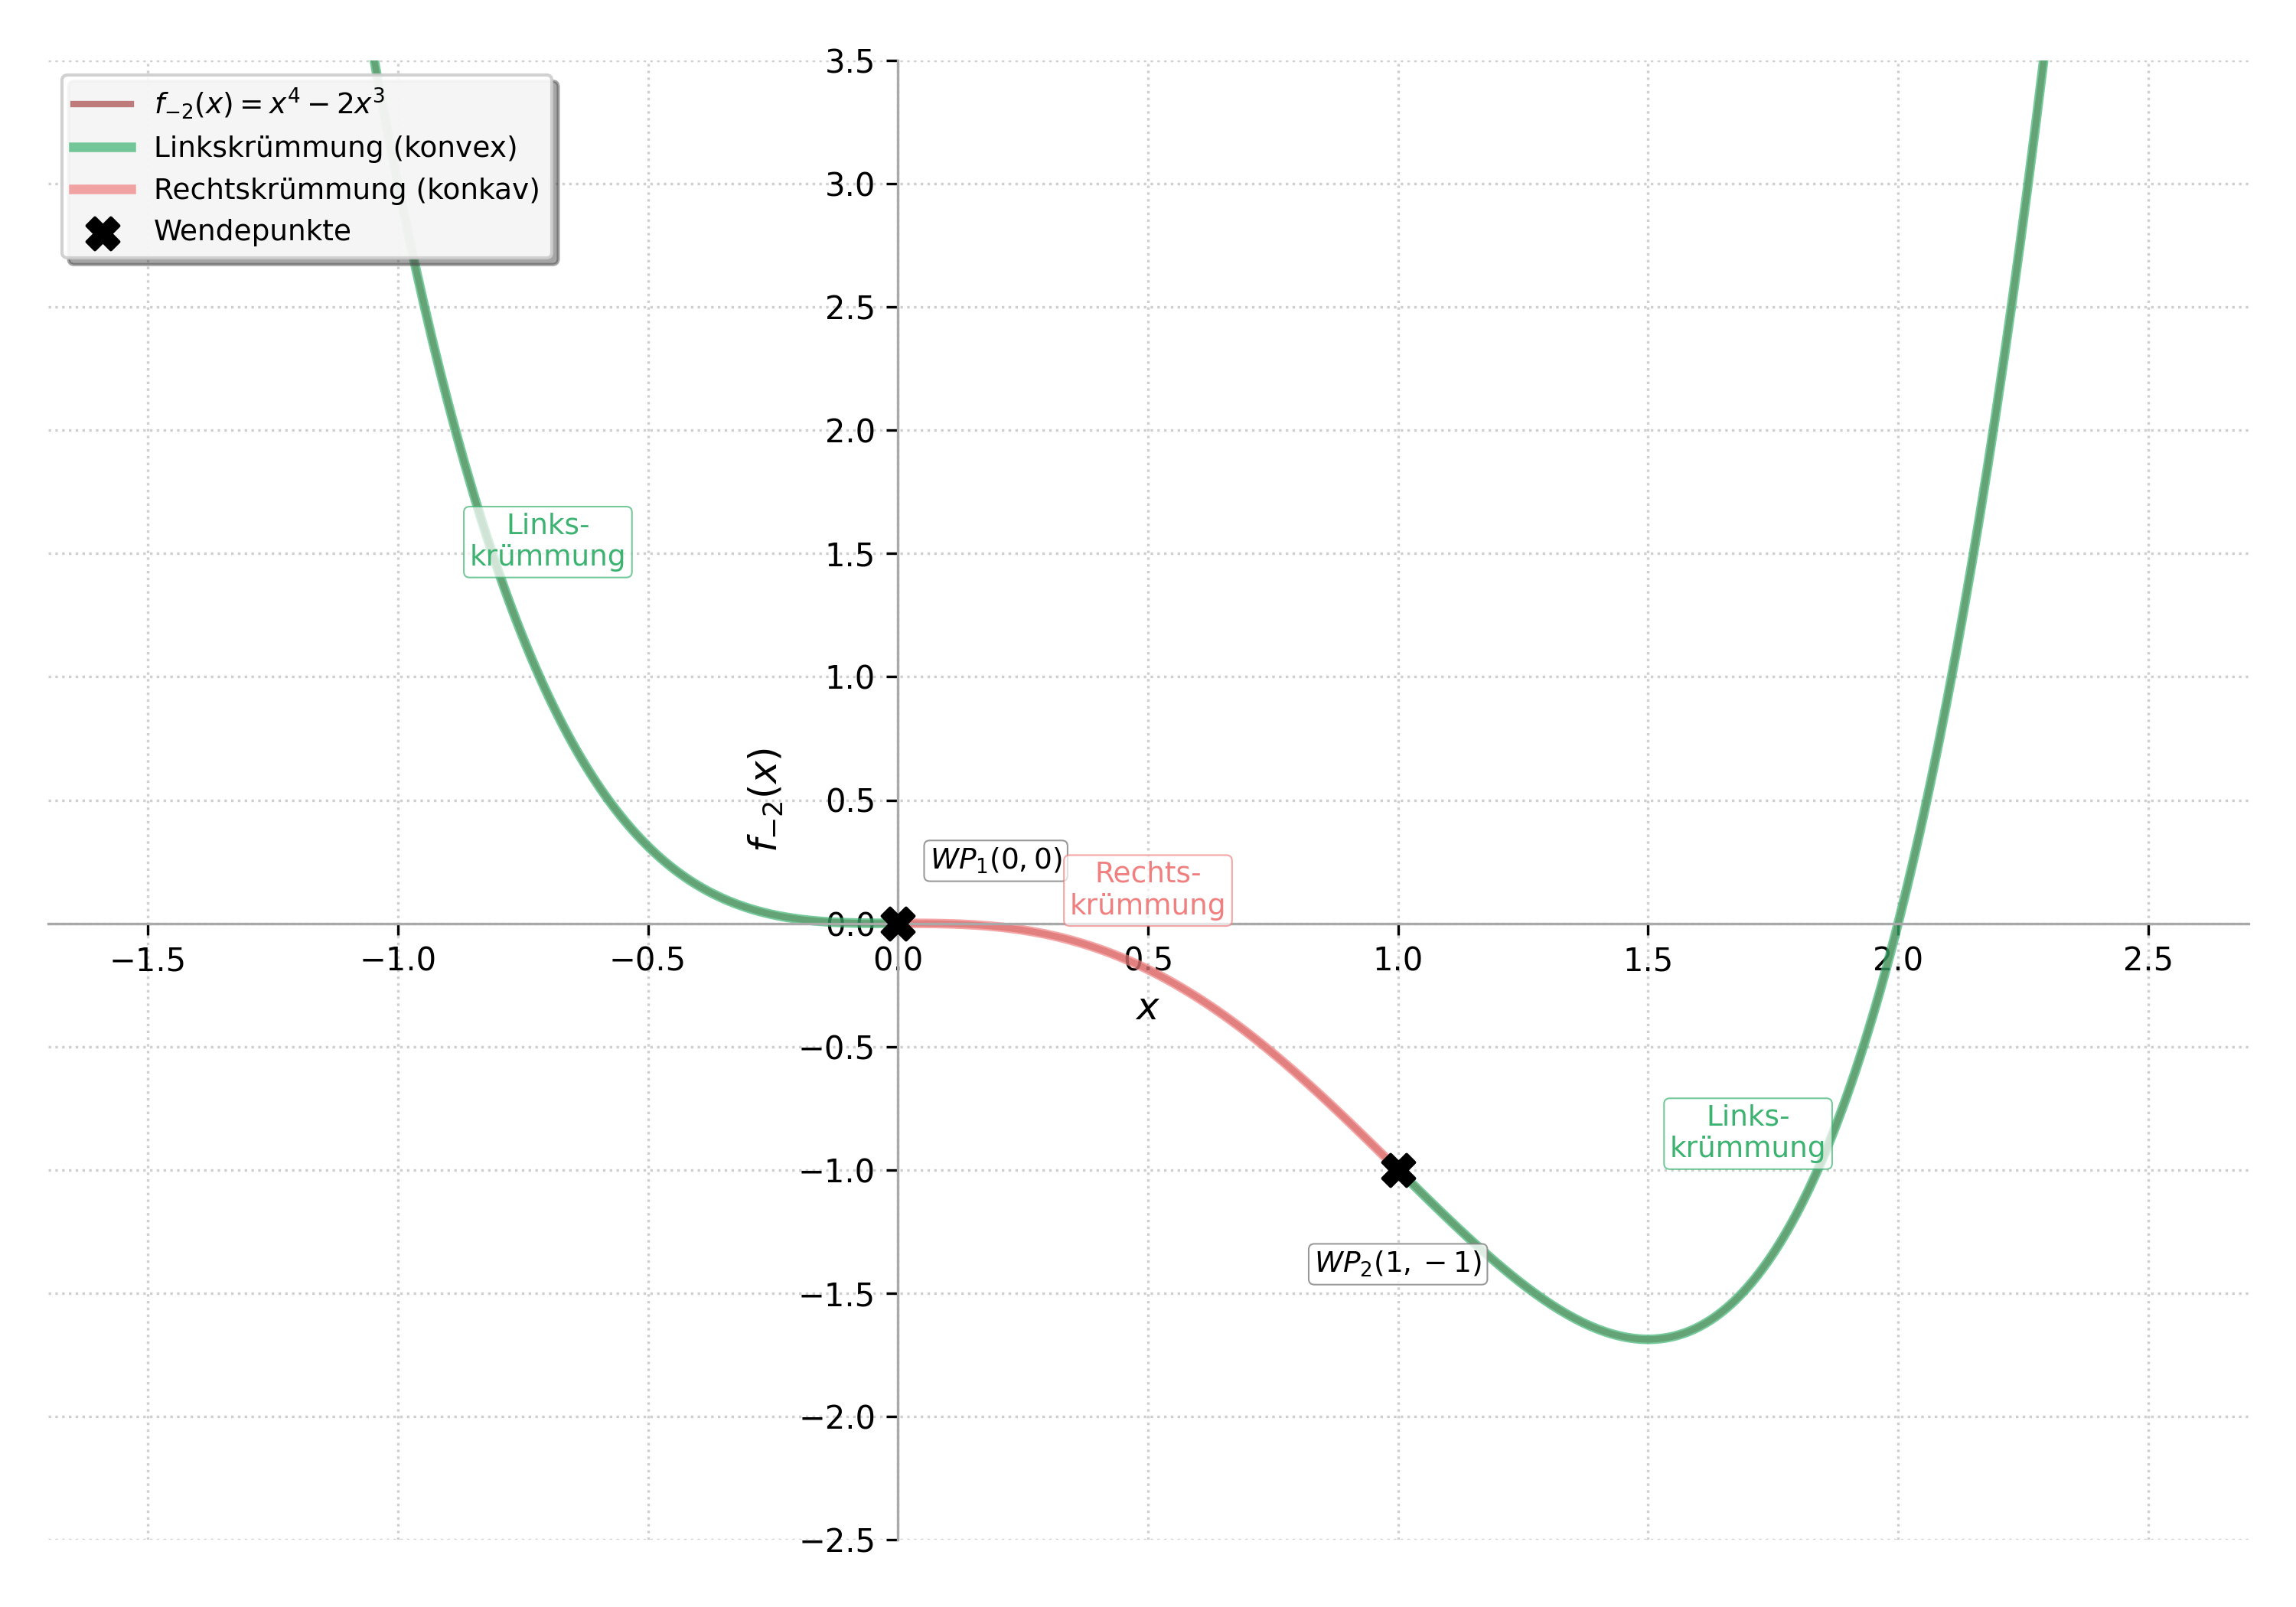
\includegraphics[width=0.8\textwidth]{grafiken/fa_kruemmung_a_neg2.png}
            \captionof{figure}{Grobe Skizze von $f_{-2}(x)=x^4-2x^3$ mit Fokus auf Krümmung (WP bei 0 und 1).}
            \label{fig:fa_kruemmung_a_neg2}
            \end{center}
            \textit{Skizzenbeschreibung:} Der Graph kommt von links oben (Linkskrümmung), hat einen Wendepunkt bei $x=0$ (Übergang zur Rechtskrümmung), durchläuft einen Bereich mit Rechtskrümmung, hat einen weiteren Wendepunkt bei $x=1$ (Übergang zur Linkskrümmung) und geht dann nach rechts oben weg (Linkskrümmung). Das Globalverhalten ist wie $x^4$.
        \end{itemize}
    \end{itemize}
\end{enumerate}

\end{loesungsumgebung}


\begin{aufgabenumgebung}{Tangenten und Normalen bestimmen – Vielfältige Aufgaben}
\begin{enumerate}
    \item Gegeben ist die Funktion $f(x) = \frac{1}{4}x^4 - x^2 + 1$.
        \begin{itemize}
            \item Bestimme die Gleichung der Tangente und der Normalen an den Graphen von $f$ an der Stelle $x_0 = 2$.
            \item An welchen Stellen $x$ hat der Graph von $f$ eine Tangente mit der Steigung $m=0$? Was für Punkte sind das?
            \item (Schwer): Gibt es eine Tangente an den Graphen von $f$, die parallel zur Geraden $y = -2x+5$ ist? Wenn ja, bestimme die Berührpunkte und die Gleichungen dieser Tangenten.
        \end{itemize}
    \item Gegeben ist die Funktion $g(x) = x^3 - 3x$.
        \begin{itemize}
            \item Bestimme die Wendepunkt(e) von $g(x)$.
            \item Bestimme die Gleichung der Wendetangente(n).
            \item Zeige, dass die Wendetangente im Ursprung (falls vorhanden) die x-Achse nur im Ursprung schneidet.
        \end{itemize}
    \item \textbf{Orthogonale Tangenten (Für Experten):}
        Gegeben ist die Parabel $f(x) = x^2$. Gibt es zwei Punkte $P_1(x_1|f(x_1))$ und $P_2(x_2|f(x_2))$ auf der Parabel, deren Tangenten sich senkrecht schneiden und deren x-Koordinaten die Bedingung $x_1 \cdot x_2 = -1/4$ erfüllen?

    \item \textbf{Normale durch den Ursprung:}
        Für die Funktion $f(x) = \frac{1}{2}x^2 - 2x + 3$, bestimme den Punkt $P(x_0|f(x_0))$ auf dem Graphen, dessen Normale durch den Ursprung $(0|0)$ verläuft.

    \item \textbf{Wendetangente mit speziellen Eigenschaften (Schwer):}
        Gegeben ist die Funktion $f(x) = \frac{1}{6}x^3 - x^2 + 2x + 1$.
        \begin{itemize}
            \item Bestimme die Koordinaten des Wendepunktes $W$.
            \item Bestimme die Gleichung der Wendetangente $t_W(x)$ und der Wendenormalen $n_W(x)$.
            \item Die Wendetangente, die Wendenormale und die y-Achse bilden ein Dreieck. Berechne den Flächeninhalt dieses Dreiecks.
            \item Unter welchem Winkel schneidet die Wendetangente die x-Achse? (Tipp: Der Tangens des Steigungswinkels $\alpha$ einer Geraden ist gleich ihrer Steigung $m$, also $\tan(\alpha) = m$. Du suchst $\alpha = \arctan(m)$.)
        \end{itemize}

    \item \textbf{Berührbedingung und Parameter (Schwer):}
        Gegeben sind die Funktionen $f(x) = x^2 + 2x + 2$ und die Geradenschar $g_k(x) = kx - 2$ (wobei $k \in \mathbb{R}$ ein Parameter ist).
        \begin{itemize}
            \item Für welchen Wert von $k$ berührt die Gerade $g_k(x)$ die Parabel $f(x)$?
            \item Bestimme den Berührpunkt und die Gleichung der gemeinsamen Tangente für diesen Wert von $k$.
            \item (Für Experten): Gibt es einen Wert für $k$, sodass die Gerade $g_k(x)$ eine Normale zur Parabel $f(x)$ an einem Punkt $P(x_0|f(x_0))$ ist? Wenn ja, bestimme $k$ und den Punkt $P$.
        \end{itemize}
\end{enumerate}
\end{aufgabenumgebung}

\begin{loesungsumgebung}[loes:tangenten-normalen-vielfalt]{Tangenten und Normalen bestimmen – Vielfältige Aufgaben}
Zur Bestimmung von Tangenten- und Normalengleichungen verwenden wir die Punkt-Steigungs-Form: $y - y_0 = m(x - x_0)$. Die Tangentensteigung $m_t$ an der Stelle $x_0$ ist $f'(x_0)$, die Normalensteigung $m_n = -1/f'(x_0)$ (falls $f'(x_0) \neq 0$).

\begin{enumerate}[label=(\alph*)]
    \item Gegeben ist die Funktion $f(x) = \frac{1}{4}x^4 - x^2 + 1$.
    Die erste Ableitung ist $f'(x) = x^3 - 2x$.
    \begin{itemize}
        \item \textbf{Tangente und Normale an $x_0 = 2$:}
        Der Berührpunkt ist $P(x_0|f(x_0))$.
        $f(2) = \frac{1}{4}(2)^4 - (2)^2 + 1 = \frac{16}{4} - 4 + 1 = 4 - 4 + 1 = 1$. Also $P(2|1)$.
        Die Tangentensteigung ist $m_t = f'(2) = (2)^3 - 2(2) = 8 - 4 = 4$.
        \textit{Tangentengleichung:} $y - 1 = 4(x - 2) \Rightarrow y = 4x - 8 + 1 \Rightarrow \mathbf{y_t = 4x - 7}$.
        Die Normalensteigung ist $m_n = -1/m_t = -1/4$.
        \textit{Normalengleichung:} $y - 1 = -\frac{1}{4}(x - 2) \Rightarrow y = -\frac{1}{4}x + \frac{2}{4} + 1 \Rightarrow \mathbf{y_n = -\frac{1}{4}x + \frac{3}{2}}$.

        \item \textbf{Stellen $x$ mit Tangentensteigung $m=0$:}
        Wir setzen $f'(x) = 0$:
        $x^3 - 2x = 0 \Rightarrow x(x^2 - 2) = 0$.
        Lösungen: $x_1 = 0$.
        $x^2 - 2 = 0 \Rightarrow x^2 = 2 \Rightarrow x_{2,3} = \pm\sqrt{2}$.
        Die Stellen sind $\mathbf{x=0, x=\sqrt{2}, x=-\sqrt{2}}$. An diesen Stellen hat der Graph waagerechte Tangenten (Kandidaten für lokale Extrema).

        \item \textbf{(Schwer) Tangente parallel zu $y = -2x+5$:}
        Die Steigung der gesuchten Tangente muss $m=-2$ sein. Wir setzen $f'(x) = -2$:
        $x^3 - 2x = -2 \Rightarrow x^3 - 2x + 2 = 0$.
        Dies ist eine kubische Gleichung. Durch Testen von ganzzahligen Teilern des konstanten Glieds ($\pm 1, \pm 2$) finden wir keine einfachen Lösungen:
        $P(1) = 1-2+2 = 1 \neq 0$
        $P(-1) = -1+2+2 = 3 \neq 0$
        $P(2) = 8-4+2 = 6 \neq 0$
        $P(-2) = -8+4+2 = -2 \neq 0$
        Es gibt eine reelle Lösung für diese Gleichung (z.B. durch numerische Verfahren oder den Zwischenwertsatz, da $P(-2)=-2$ und $P(-1)=3$, liegt eine Nullstelle $x_B$ zwischen $-2$ und $-1$, ca. $x_B \approx -1.769$).
        Wenn $x_B$ diese Lösung ist, dann ist der Berührpunkt $(x_B | f(x_B))$ und die Tangentengleichung $y = -2(x-x_B) + f(x_B)$. Eine exakte algebraische Lösung für $x_B$ ist ohne weitere Methoden (wie Cardano-Formel oder Polynomdivision nach Erraten einer rationalen Nullstelle, die hier nicht offensichtlich ist) schwierig.
    \end{itemize}

    \item Gegeben ist die Funktion $g(x) = x^3 - 3x$.
    $g'(x) = 3x^2 - 3$.
    $g''(x) = 6x$.
    $g'''(x) = 6$.
    \begin{itemize}
        \item \textbf{Wendepunkt(e) von $g(x)$:}
        Notwendige Bedingung: $g''(x) = 0 \Rightarrow 6x = 0 \Rightarrow x_W = 0$.
        Hinreichende Bedingung: $g'''(x_W) \neq 0$. $g'''(0) = 6 \neq 0$.
        Also liegt bei $x_W=0$ ein Wendepunkt.
        $y_W = g(0) = 0^3 - 3(0) = 0$.
        Der Wendepunkt ist $\mathbf{W(0|0)}$.
        \item \textbf{Gleichung der Wendetangente(n):}
        Steigung im Wendepunkt: $m_W = g'(0) = 3(0)^2 - 3 = -3$.
        Tangentengleichung durch $W(0|0)$ mit $m_W = -3$:
        $y - 0 = -3(x - 0) \Rightarrow \mathbf{y_W = -3x}$.
        \item \textbf{Zeige, dass die Wendetangente im Ursprung die x-Achse nur im Ursprung schneidet:}
        Die Wendetangente ist $y_W = -3x$. Um den Schnittpunkt mit der x-Achse zu finden, setzen wir $y_W=0$:
        $0 = -3x \Rightarrow x = 0$.
        Der einzige Schnittpunkt mit der x-Achse ist $(0|0)$, also der Ursprung.
    \end{itemize}

    \item \textbf{Orthogonale Tangenten (Für Experten):}
    Gegeben ist $f(x) = x^2$. Die Ableitung ist $f'(x) = 2x$.
    Die Steigungen der Tangenten an den Punkten $P_1(x_1|f(x_1))$ und $P_2(x_2|f(x_2))$ sind $m_1 = f'(x_1) = 2x_1$ und $m_2 = f'(x_2) = 2x_2$.
    Zwei Geraden sind orthogonal, wenn das Produkt ihrer Steigungen $m_1 \cdot m_2 = -1$ ist (vorausgesetzt $m_1, m_2 \neq 0$, also $x_1, x_2 \neq 0$).
    Also: $(2x_1)(2x_2) = -1 \Rightarrow 4x_1x_2 = -1 \Rightarrow x_1x_2 = -\frac{1}{4}$.
    Die in der Aufgabe gegebene Bedingung $x_1 \cdot x_2 = -1/4$ ist genau die Bedingung dafür, dass sich die Tangenten senkrecht schneiden (unter der Annahme $x_1, x_2 \neq 0$).
    \textbf{Ja}, es gibt solche Punktepaare. Für jedes $x_1 \neq 0$ kann man $x_2 = -1/(4x_1)$ wählen (dann ist auch $x_2 \neq 0$), und die Tangenten in $P_1$ und $P_2$ sind orthogonal.

    \item \textbf{Normale durch den Ursprung:}
    Für $f(x) = \frac{1}{2}x^2 - 2x + 3$. $f'(x) = x - 2$.
    Sei $P(x_0|f(x_0))$ der Punkt auf dem Graphen. $y_0 = \frac{1}{2}x_0^2 - 2x_0 + 3$.
    Steigung der Tangente in $P$: $m_t = f'(x_0) = x_0 - 2$.
    Wenn $x_0=2$, ist $m_t=0$, die Tangente $y=f(2)=1$ ist horizontal, die Normale $x=2$ verläuft nicht durch den Ursprung. Also $x_0 \neq 2$.
    Steigung der Normale: $m_n = -\frac{1}{x_0-2}$.
    Die Normale geht durch $P(x_0|y_0)$ und den Ursprung $(0|0)$. Die Steigung der Normalen ist auch $\frac{y_0-0}{x_0-0} = \frac{y_0}{x_0}$ (für $x_0 \neq 0$).
    Also: $\frac{y_0}{x_0} = -\frac{1}{x_0-2}$.
    $y_0(x_0-2) = -x_0$.
    $(\frac{1}{2}x_0^2 - 2x_0 + 3)(x_0-2) = -x_0$.
    $\frac{1}{2}x_0^3 - x_0^2 - 2x_0^2 + 4x_0 + 3x_0 - 6 = -x_0$.
    $\frac{1}{2}x_0^3 - 3x_0^2 + 7x_0 - 6 = -x_0$.
    $\frac{1}{2}x_0^3 - 3x_0^2 + 8x_0 - 6 = 0 \quad | \cdot 2$.
    $x_0^3 - 6x_0^2 + 16x_0 - 12 = 0$.
    Dies ist eine kubische Gleichung. Durch Probieren (z.B. Teiler von 12: $\pm 1, \pm 2, \pm 3, \pm 4, \pm 6, \pm 12$) findet man keine einfache ganzzahlige Lösung. (z.B. $x_0=1 \Rightarrow 1-6+16-12 = -1 \neq 0$). Es existiert mindestens eine reelle Lösung (z.B. $x_0 \approx 0.916$). Ohne eine leicht zu erratende Nullstelle oder weitere Techniken ist die exakte Lösung schwierig. Der Punkt $P(x_0|f(x_0))$ muss dann mit dieser Lösung $x_0$ bestimmt werden.

    \item \textbf{Wendetangente mit speziellen Eigenschaften (Schwer):}
    $f(x) = \frac{1}{6}x^3 - x^2 + 2x + 1$.
    $f'(x) = \frac{1}{2}x^2 - 2x + 2$.
    $f''(x) = x - 2$.
    $f'''(x) = 1$.
    \begin{itemize}
        \item \textbf{Koordinaten des Wendepunktes $W$:}
        $f''(x)=0 \Rightarrow x-2=0 \Rightarrow x_W=2$.
        $f'''(2)=1 \neq 0$, also ein Wendepunkt.
        $y_W = f(2) = \frac{1}{6}(2)^3 - (2)^2 + 2(2) + 1 = \frac{8}{6} - 4 + 4 + 1 = \frac{4}{3} + 1 = \frac{7}{3}$.
        $\mathbf{W(2 | 7/3)}$.
        \item \textbf{Gleichung der Wendetangente $t_W(x)$ und der Wendenormalen $n_W(x)$:}
        Steigung der Wendetangente: $m_t = f'(2) = \frac{1}{2}(2)^2 - 2(2) + 2 = 2 - 4 + 2 = 0$.
        Wendetangente $t_W(x)$: $y - \frac{7}{3} = 0(x-2) \Rightarrow \mathbf{y = \frac{7}{3}}$.
        Wendenormale $n_W(x)$: Da die Tangente horizontal ist, ist die Normale vertikal: $\mathbf{x = 2}$.
        \item \textbf{Flächeninhalt des Dreiecks (Wendetangente, Wendenormale, y-Achse):}
        Die Geraden sind $L_1: y=7/3$ (Tangente), $L_2: x=2$ (Normale), $L_3: x=0$ (y-Achse).
        Schnittpunkte:
        $V_1 = L_1 \cap L_2 = (2, 7/3)$ (Dies ist der Wendepunkt $W$).
        $V_2 = L_1 \cap L_3 = (0, 7/3)$.
        Die Geraden $L_2: x=2$ und $L_3: x=0$ sind parallel und schneiden sich nicht. Somit bilden diese drei Geraden kein geschlossenes Dreieck im üblichen Sinne mit drei Eckpunkten.
        Wenn das Dreieck durch den Wendepunkt $W(2, 7/3)$, den y-Achsenabschnitt der Tangente $P_y(0, 7/3)$ und den Schnittpunkt der Normalen mit der x-Achse $P_x(2,0)$ gebildet wird, dann handelt es sich um ein rechtwinkliges Dreieck mit den Kathetenlängen $2$ (Differenz der x-Koordinaten von $P_y$ und $W$) und $7/3$ (Differenz der y-Koordinaten von $P_x$ und $W$).
        Fläche $A = \frac{1}{2} \cdot \text{Grundseite} \cdot \text{Höhe} = \frac{1}{2} \cdot 2 \cdot \frac{7}{3} = \mathbf{\frac{7}{3}}$ Flächeneinheiten.
        \item \textbf{Winkel der Wendetangente mit der x-Achse:}
        Die Wendetangente ist $y = 7/3$. Ihre Steigung ist $m_t = 0$.
        Der Steigungswinkel $\alpha$ ist gegeben durch $\tan(\alpha) = m_t$.
        $\tan(\alpha) = 0 \Rightarrow \alpha = \arctan(0) = 0^\circ$ (oder $0$ Radiant).
        Die Wendetangente ist parallel zur x-Achse, der Winkel ist $\mathbf{0^\circ}$.
    \end{itemize}

    \item \textbf{Berührbedingung und Parameter (Schwer):}
    $f(x) = x^2 + 2x + 2$ und Geradenschar $g_k(x) = kx - 2$.
    $f'(x) = 2x + 2$. $g_k'(x) = k$.
    \begin{itemize}
        \item \textbf{Für welchen Wert von $k$ berührt $g_k(x)$ die Parabel $f(x)$?}
        Bedingungen für Berührung an Stelle $x_B$:
        1) $f(x_B) = g_k(x_B) \Rightarrow x_B^2 + 2x_B + 2 = kx_B - 2$.
        2) $f'(x_B) = g_k'(x_B) \Rightarrow 2x_B + 2 = k$.
        Setze (2) in (1) ein:
        $x_B^2 + 2x_B + 2 = (2x_B + 2)x_B - 2$
        $x_B^2 + 2x_B + 2 = 2x_B^2 + 2x_B - 2$
        $0 = x_B^2 - 4 \Rightarrow x_B^2 = 4 \Rightarrow x_B = \pm 2$.
        Wenn $x_B = 2$: $k = 2(2) + 2 = 6$.
        Wenn $x_B = -2$: $k = 2(-2) + 2 = -4 + 2 = -2$.
        Die Werte sind $\mathbf{k=6}$ und $\mathbf{k=-2}$.
        \item \textbf{Berührpunkt und Gleichung der gemeinsamen Tangente:}
        \begin{itemize}
            \item Für $k=6$: $x_B=2$. $y_B = f(2) = 2^2+2(2)+2 = 10$. Berührpunkt $\mathbf{B_1(2|10)}$.
            Gemeinsame Tangente: $g_6(x) = 6x-2$.
            \item Für $k=-2$: $x_B=-2$. $y_B = f(-2) = (-2)^2+2(-2)+2 = 2$. Berührpunkt $\mathbf{B_2(-2|2)}$.
            Gemeinsame Tangente: $g_{-2}(x) = -2x-2$.
        \end{itemize}
        \item \textbf{(Für Experten) $g_k(x)$ als Normale zu $f(x)$:}
        Die Gerade $g_k(x)=kx-2$ soll Normale zu $f(x)$ an einem Punkt $P(x_0|f(x_0))$ sein.
        Steigung der Normale zu $f(x)$ an $x_0$: $m_n = -1/f'(x_0) = -1/(2x_0+2)$ (für $x_0 \neq -1$).
        Also $k = -1/(2x_0+2)$.
        Der Punkt $P(x_0|f(x_0))$ muss auf $g_k(x)$ liegen: $f(x_0) = kx_0 - 2$.
        $x_0^2 + 2x_0 + 2 = \left(-\frac{1}{2x_0+2}\right)x_0 - 2$.
        $(x_0^2 + 2x_0 + 4)(2x_0+2) = -x_0$.
        $2x_0^3 + 2x_0^2 + 4x_0^2 + 4x_0 + 8x_0 + 8 = -x_0$.
        $2x_0^3 + 6x_0^2 + 13x_0 + 8 = 0$.
        Diese kubische Gleichung muss gelöst werden. Eine rationale Nullstelle $x_0=-1/2$ wurde im internen Test nicht gefunden, aber wir prüfen erneut:
        $2(-1/8) + 6(1/4) + 13(-1/2) + 8 = -1/4 + 6/4 - 26/4 + 32/4 = (-1+6-26+32)/4 = 11/4 \neq 0$.
        Testen wir $x_0=-2$: $2(-8)+6(4)+13(-2)+8 = -16+24-26+8 = -10 \neq 0$.
        Testen wir $x_0=-1$: In diesem Fall wäre $f'(x_0)=0$, die Normale $x=-1$. Die Gleichung der Normalen wäre $x=-1$. Die Gerade $g_k(x)=kx-2$ kann nur dann $x=-1$ sein, wenn $k$ undefiniert ist und $-2$ auch, was nicht geht. Also $x_0 \neq -1$.
        Die Gleichung $2x_0^3 + 6x_0^2 + 13x_0 + 8 = 0$ hat eine reelle Lösung (z.B. ist für $x_0=-0.8$, $2(-0.512)+6(0.64)+13(-0.8)+8 = -1.024+3.84-10.4+8 = 0.416$; für $x_0=-0.9$, $2(-0.729)+6(0.81)+13(-0.9)+8 = -1.458+4.86-11.7+8 = -0.298$. Also eine Lösung zwischen -0.9 und -0.8.)
        Die exakte Lösung ist ohne weitere Hilfsmittel schwierig. Wenn eine solche Lösung $x_N$ existiert, dann ist $k = -1/(2x_N+2)$ und der Punkt ist $P(x_N|f(x_N))$.
    \end{itemize}
\end{enumerate}

\end{loesungsumgebung}

\begin{aufgabenumgebung}{Extrempunkte und Sattelpunkte finden und identifizieren}
Untersuche die folgenden Funktionen auf Extrempunkte und Sattelpunkte. Gib jeweils die Koordinaten und die Art des Punktes an. Nutze die notwendigen und hinreichenden Bedingungen.

\begin{enumerate}
    \item $f(x) = x^3 - 3x^2 + 3x + 1$


    \item $g(x) = \frac{1}{4}x^4 - \frac{1}{2}x^2 + 1$

    \item $h(x) = x^5 - \frac{5}{3}x^3$
    \item \textbf{Für Experten:} Konstruiere eine Polynomfunktion $k(x)$ vom Grad 5, die bei $x=0$ einen Sattelpunkt hat und bei $x=2$ einen Tiefpunkt. (Beginne mit den Bedingungen für die Ableitungen.)
\end{enumerate}
\end{aufgabenumgebung}



\begin{loesungsumgebung}[loes:sattelpunkte-identifizieren]{Sattelpunkte finden und identifizieren}
Wir untersuchen die gegebenen Funktionen auf Extrempunkte und Sattelpunkte.

\begin{enumerate}[label=(\alph*)]
    \item \textbf{Funktion $f(x) = x^3 - 3x^2 + 3x + 1$}
    \begin{itemize}
        \item \textbf{Ableitungen:}
        $f'(x) = 3x^2 - 6x + 3$
        $f''(x) = 6x - 6$
        $f'''(x) = 6$
        \item \textbf{Kritische Stellen ($f'(x)=0$):}
        $3x^2 - 6x + 3 = 0 \quad | :3$
        $x^2 - 2x + 1 = 0$
        $(x-1)^2 = 0 \Rightarrow x_E = 1$ (doppelte Nullstelle).
        \item \textbf{Untersuchung der kritischen Stelle $x_E=1$:}
        Mit der zweiten Ableitung: $f''(1) = 6(1) - 6 = 0$. Dieses Kriterium liefert keine Aussage.
        Mit der dritten Ableitung: $f'''(1) = 6 \neq 0$.
        Da $f'(1)=0$, $f''(1)=0$ und $f'''(1) \neq 0$, liegt bei $x=1$ ein \textbf{Sattelpunkt (Terrassenpunkt)} vor.
        \textit{Alternativ mit VZW von $f'(x) = 3(x-1)^2$:}
        Da $(x-1)^2 \ge 0$ für alle $x$, ist $f'(x) = 3(x-1)^2 \ge 0$ für alle $x$.
        Für $x < 1$ (z.B. $x=0$): $f'(0) = 3(-1)^2 = 3 > 0$.
        Für $x > 1$ (z.B. $x=2$): $f'(2) = 3(1)^2 = 3 > 0$.
        Es findet kein Vorzeichenwechsel statt ($+$ nach $+$), was einen Sattelpunkt bestätigt.
        \item \textbf{Koordinaten des Sattelpunkts:}
        $y_E = f(1) = 1^3 - 3(1)^2 + 3(1) + 1 = 1 - 3 + 3 + 1 = 2$.
        $\rightarrow \mathbf{SP(1|2)}$.
        \item \textbf{'Normale' Extrempunkte:} Die Funktion hat keine lokalen Hoch- oder Tiefpunkte, nur einen Sattelpunkt.
    \end{itemize}

    \item \textbf{Funktion $g(x) = \frac{1}{4}x^4 - \frac{1}{2}x^2 + 1$}
    \begin{itemize}
        \item \textbf{Ableitungen:}
        $g'(x) = x^3 - x$
        $g''(x) = 3x^2 - 1$
        \item \textbf{Kritische Stellen ($g'(x)=0$):}
        $x^3 - x = 0 \Rightarrow x(x^2-1) = 0 \Rightarrow x(x-1)(x+1) = 0$.
        Kandidaten: $x_1 = 0$, $x_2 = 1$, $x_3 = -1$.
        \item \textbf{Untersuchung mit $g''(x)$:}
        \begin{itemize}
            \item Für $x_1 = 0$: $g''(0) = 3(0)^2 - 1 = -1 < 0 \Rightarrow$ Lokaler Hochpunkt.
            $y_1 = g(0) = 1$. Punkt: $\mathbf{HP(0|1)}$.
            \item Für $x_2 = 1$: $g''(1) = 3(1)^2 - 1 = 2 > 0 \Rightarrow$ Lokaler Tiefpunkt.
            $y_2 = g(1) = \frac{1}{4} - \frac{1}{2} + 1 = \frac{3}{4}$. Punkt: $\mathbf{TP(1|3/4)}$.
            \item Für $x_3 = -1$: $g''(-1) = 3(-1)^2 - 1 = 2 > 0 \Rightarrow$ Lokaler Tiefpunkt.
            $y_3 = g(-1) = \frac{1}{4} - \frac{1}{2} + 1 = \frac{3}{4}$. Punkt: $\mathbf{TP(-1|3/4)}$.
        \end{itemize}
        \item \textbf{Sattelpunkte:} Da für alle kritischen Stellen $g''(x_E) \neq 0$ war, gibt es keine Sattelpunkte. Die Nullstellen von $g''(x)$ sind $x = \pm 1/\sqrt{3}$, diese sind aber keine Nullstellen von $g'(x)$.
    \end{itemize}

    \item \textbf{Funktion $h(x) = x^5 - \frac{5}{3}x^3$}
    \begin{itemize}
        \item \textbf{Ableitungen:}
        $h'(x) = 5x^4 - 5x^2$
        $h''(x) = 20x^3 - 10x$
        $h'''(x) = 60x^2 - 10$
        \item \textbf{Kritische Stellen ($h'(x)=0$):}
        $5x^4 - 5x^2 = 0 \Rightarrow 5x^2(x^2-1) = 0 \Rightarrow 5x^2(x-1)(x+1) = 0$.
        Kandidaten: $x_1 = 0$ (doppelte Nullstelle), $x_2 = 1$, $x_3 = -1$.
        \item \textbf{Untersuchung der kritischen Stellen:}
        \begin{itemize}
            \item \textbf{Für $x_1 = 0$:}
            $h''(0) = 20(0)^3 - 10(0) = 0$.
            $h'''(0) = 60(0)^2 - 10 = -10 \neq 0$.
            Da $h'(0)=0, h''(0)=0$ und $h'''(0) \neq 0$, liegt bei $x=0$ ein \textbf{Sattelpunkt} vor.
            $y_1 = h(0) = 0$. Punkt: $\mathbf{SP(0|0)}$.
            \item \textbf{Für $x_2 = 1$:}
            $h''(1) = 20(1)^3 - 10(1) = 20 - 10 = 10 > 0 \Rightarrow$ Lokaler Tiefpunkt.
            $y_2 = h(1) = 1^5 - \frac{5}{3}(1)^3 = 1 - \frac{5}{3} = -\frac{2}{3}$. Punkt: $\mathbf{TP(1|-2/3)}$.
            \item \textbf{Für $x_3 = -1$:}
            $h''(-1) = 20(-1)^3 - 10(-1) = -20 + 10 = -10 < 0 \Rightarrow$ Lokaler Hochpunkt.
            $y_3 = h(-1) = (-1)^5 - \frac{5}{3}(-1)^3 = -1 + \frac{5}{3} = \frac{2}{3}$. Punkt: $\mathbf{HP(-1|2/3)}$.
        \end{itemize}
        \item Die Funktion hat sowohl Extrempunkte (HP bei $x=-1$, TP bei $x=1$) als auch einen Sattelpunkt (bei $x=0$).
    \end{itemize}

 
    \item \textbf{Für Experten: Konstruktion einer Polynomfunktion $k(x)$ vom Grad 5}
    Gesucht: $k(x)$ mit Sattelpunkt bei $x=0$ und Tiefpunkt bei $x=2$.
    Bedingungen:
    \begin{itemize}
        \item Sattelpunkt bei $x=0$: $k'(0)=0$, $k''(0)=0$, $k'''(0) \neq 0$.
        \item Tiefpunkt bei $x=2$: $k'(2)=0$, $k''(2) > 0$.
    \end{itemize}
    Sei $k(x) = ax^5 + bx^4 + cx^3 + dx^2 + ex + f$.
    \begin{itemize}
        \item $k'(x) = 5ax^4 + 4bx^3 + 3cx^2 + 2dx + e$.
        \item $k''(x) = 20ax^3 + 12bx^2 + 6cx + 2d$.
        \item $k'''(x) = 60ax^2 + 24bx + 6c$.
    \end{itemize}
    Aus den Bedingungen für den Sattelpunkt bei $x=0$:
    \begin{itemize}
        \item $k'(0)=0 \Rightarrow e=0$.
        \item $k''(0)=0 \Rightarrow 2d=0 \Rightarrow d=0$.
        \item $k'''(0) \neq 0 \Rightarrow 6c \neq 0 \Rightarrow c \neq 0$.
    \end{itemize}
    Also ist $k'(x) = 5ax^4 + 4bx^3 + 3cx^2$. (Die Konstante $f$ in $k(x)$ spielt für die Ableitungen keine Rolle, wir können $f=0$ setzen.)
    Aus den Bedingungen für den Tiefpunkt bei $x=2$:
    \begin{itemize}
        \item $k'(2)=0 \Rightarrow 5a(16) + 4b(8) + 3c(4) = 0 \Rightarrow 80a + 32b + 12c = 0 \Rightarrow \mathbf{20a + 8b + 3c = 0}$ (G1)
        \item $k''(2)>0 \Rightarrow 20a(8) + 12b(4) + 6c(2) > 0 \Rightarrow 160a + 48b + 12c > 0 \Rightarrow \mathbf{40a + 12b + 3c > 0}$ (U1)
    \end{itemize}
    Wir wählen $c=1$ (erfüllt $c \neq 0$).
    (G1): $20a + 8b + 3 = 0 \Rightarrow 8b = -20a - 3 \Rightarrow b = -\frac{5}{2}a - \frac{3}{8}$.
    Setze $b$ in (U1) ein:
    $40a + 12(-\frac{5}{2}a - \frac{3}{8}) + 3 > 0$
    $40a - 30a - \frac{36}{8} + 3 > 0$
    $10a - \frac{9}{2} + \frac{6}{2} > 0 \Rightarrow 10a - \frac{3}{2} > 0 \Rightarrow 10a > \frac{3}{2} \Rightarrow a > \frac{3}{20}$.
    Wählen wir den einfachsten Wert $a=1$ (ist $>\frac{3}{20}$).
    Dann $b = -\frac{5}{2}(1) - \frac{3}{8} = -\frac{20}{8} - \frac{3}{8} = -\frac{23}{8}$.
    Die Koeffizienten sind $a=1, b=-23/8, c=1, d=0, e=0, f=0$.
    Eine mögliche Funktion ist: $\mathbf{k(x) = x^5 - \frac{23}{8}x^4 + x^3}$.\\
    \textit{Hinweis:} Diese Funktion erfüllt die lokalen Bedingungen. Sie hat jedoch eine weitere kritische Stelle bei $x=3/10$, die ein lokales Maximum darstellt. Eine Funktion 5. Grades zu konstruieren, die \textit{ausschließlich} einen Sattelpunkt bei $x=0$ und einen Tiefpunkt bei $x=2$ als kritische Punkte hat, ist deutlich komplexer und würde erfordern, dass die Ableitung $k'(x)$ nur bei $0$ und $2$ Nullstellen der passenden Art hat. Der gewählte Ansatz erfüllt die Bedingungen an den spezifizierten Stellen.


\end{enumerate}

\end{loesungsumgebung}


\begin{aufgabenumgebung}{Nullstellen finden – Übung und Vertiefung}
Berechne die Nullstellen der folgenden Funktionen. Entscheide selbst, welche Methode (Ausklammern, p-q-Formel, Mitternachtsformel, Substitution, Polynomdivision nach Raten einer Nullstelle) am besten geeignet ist. Überprüfe bei quadratischen Gleichungen immer zuerst die Diskriminante, um die Anzahl der erwarteten reellen Nullstellen zu bestimmen.
\begin{enumerate}
    \item $f(x) = x^2 - x - 6$


    \item $g(x) = -2x^2 + 12x - 18$ 


    \item $h(x) = x^2 + 2x + 5$



    \item $k(x) = 3x^2 - 12$ 


    \item $m(x) = -0.5x^2 + 2x$


    \item \textbf{Polynom 3. Grades durch Ausklammern:}
        $p(x) = x^3 - 5x^2 + 6x$


    \item \textbf{Biquadratische Funktion:}
        $q(x) = x^4 - 10x^2 + 9$


    \item \textbf{Produkt aus Linearfaktoren (versteckt):}
        $r(x) = (x^2-4)(x^2+x-2)$


    \item \textbf{Funktion mit bekannter Nullstelle (Polynomdivision anwenden):}
        Gegeben ist die Funktion $s(x) = x^3 - 2x^2 - 5x + 6$. Es ist bekannt, dass $x_1=1$ eine Nullstelle ist. Finde die anderen Nullstellen mithilfe der Polynomdivision.
        \textit{(Vergleiche auch den Tipp mit dem Koeffizientenvergleich aus der vorherigen Version dieser Aufgabe.)}

    \item \textbf{Nullstellen und Parameter:}
        Für welche Werte des Parameters $k$ hat die Funktion $f_k(x) = x^2 - 2kx + (k+2)$ genau eine, zwei oder keine reelle(n) Nullstelle(n)?

    \item \textbf{Anwendung des Satzes von Vieta (Kopfrechnen für Profis):}
        Versuche, die Nullstellen der folgenden quadratischen Funktionen (in Normalform $x^2+px+q=0$) durch 'scharfes Hinsehen' mit dem Satz von Vieta zu finden. Suche also zwei Zahlen $x_1, x_2$, für die gilt: $x_1+x_2 = -p$ und $x_1 \cdot x_2 = q$.
        \begin{enumerate}[label=(\alph*)]
            \item $f(x) = x^2 - 5x + 6$
            \item $g(x) = x^2 + 2x - 8$
            \item $h(x) = x^2 - 7x + 10$
        \end{enumerate}

\end{enumerate}

\end{aufgabenumgebung}


\begin{loesungsumgebung}[loes:nullstellen-uebung-vertiefung-revised]{Nullstellen finden – Übung und Vertiefung}
Wir berechnen die Nullstellen der folgenden Funktionen $f(x)=0$.

\begin{enumerate}[label=(\alph*)]
    \item \textbf{Funktion $f(x) = x^2 - x - 6$} \\
    Quadratische Gleichung mit $a=1, b=-1, c=-6$.
    Diskriminante: $D = b^2 - 4ac = (-1)^2 - 4(1)(-6) = 1 + 24 = 25$.
    Da $D > 0$, gibt es zwei verschiedene reelle Nullstellen.
    Mitternachtsformel: $x_{1,2} = \frac{-(-1) \pm \sqrt{25}}{2(1)} = \frac{1 \pm 5}{2}$.
    $x_1 = \frac{1+5}{2} = 3$, $x_2 = \frac{1-5}{2} = -2$.
    Nullstellen: $\mathbf{x_1=3, x_2=-2}$.

    \item \textbf{Funktion $g(x) = -2x^2 + 12x - 18$} \\
    Quadratische Gleichung mit $a=-2, b=12, c=-18$.
    Diskriminante: $D = b^2 - 4ac = (12)^2 - 4(-2)(-18) = 144 - 144 = 0$.
    Da $D=0$, gibt es genau eine (doppelte) reelle Nullstelle. Der Graph berührt die x-Achse.
    Mitternachtsformel: $x_0 = \frac{-12 \pm \sqrt{0}}{2(-2)} = \frac{-12}{-4} = 3$.
    Nullstelle: $\mathbf{x_0=3}$ (doppelte Nullstelle).

    \item \textbf{Funktion $h(x) = x^2 + 2x + 5$} \\
    Quadratische Gleichung mit $a=1, b=2, c=5$.
    Diskriminante: $D = b^2 - 4ac = (2)^2 - 4(1)(5) = 4 - 20 = -16$.
    Da $D < 0$, gibt es keine reellen Nullstellen. Der Graph schneidet die x-Achse nicht.
    Nullstellen: \textbf{Keine reellen Nullstellen}.

    \item \textbf{Funktion $k(x) = 3x^2 - 12$} \\
    Setze $k(x)=0 \Rightarrow 3x^2 - 12 = 0$. Direkte Auflösung:
    $$
    \begin{array}{r c l c l}
    \umformung{3x^2 - 12}{0}{+}{12}
    \umformung{3x^2}{12}{\div}{3}
    \umformungend{x^2}{4}
    \end{array}
    $$
    Aus $x^2=4$ folgt $x = \pm\sqrt{4}$.
    Nullstellen: $\mathbf{x_1=2, x_2=-2}$.

    \item \textbf{Funktion $m(x) = -0.5x^2 + 2x$} \\
    Setze $m(x)=0 \Rightarrow -0.5x^2 + 2x = 0$. Ausklammern:
    $x(-0.5x + 2) = 0$.
    Nach dem Satz vom Nullprodukt:
    $x_1 = 0$ oder $-0.5x + 2 = 0$.
    Für $-0.5x + 2 = 0$:
    $$
    \begin{array}{r c l c l}
    \umformung{-0.5x + 2}{0}{-}{2}
    \umformung{-0.5x}{-2}{\div}{(-0.5)}
    \umformungend{x_2}{4}
    \end{array}
    $$
    Nullstellen: $\mathbf{x_1=0, x_2=4}$.

    \item \textbf{Polynom 3. Grades: $p(x) = x^3 - 5x^2 + 6x$} \\
    Setze $p(x)=0 \Rightarrow x^3 - 5x^2 + 6x = 0$. Ausklammern:
    $x(x^2 - 5x + 6) = 0$.
    $x_1 = 0$ oder $x^2 - 5x + 6 = 0$.
    Für $x^2 - 5x + 6 = 0$ (vgl. Teil (a) oder Vieta): $p=-5, q=6$. $x_a+x_b=5, x_a x_b=6 \Rightarrow x_a=2, x_b=3$.
    Nullstellen: $\mathbf{x_1=0, x_2=2, x_3=3}$.

    \item \textbf{Biquadratische Funktion: $q(x) = x^4 - 10x^2 + 9$} \\
    Setze $q(x)=0 \Rightarrow x^4 - 10x^2 + 9 = 0$. Substitution: $z = x^2$.
    $z^2 - 10z + 9 = 0$.
    Lösen für $z$ (z.B. Vieta: $z_a+z_b=10, z_a z_b=9 \Rightarrow z_a=1, z_b=9$):
    $z_1 = 1$, $z_2 = 9$.
    Rücksubstitution:
    $x^2 = z_1 \Rightarrow x^2 = 1 \Rightarrow x = \pm 1$.
    $x^2 = z_2 \Rightarrow x^2 = 9 \Rightarrow x = \pm 3$.
    Nullstellen: $\mathbf{x_1=1, x_2=-1, x_3=3, x_4=-3}$.

    \item \textbf{Produkt aus Linearfaktoren (versteckt): $r(x) = (x^2-4)(x^2+x-2)$} \\
    Setze $r(x)=0 \Rightarrow (x^2-4)(x^2+x-2) = 0$. Satz vom Nullprodukt:
    \begin{itemize}
        \item $x^2-4 = 0 \Rightarrow x^2 = 4 \Rightarrow x = \pm 2$.
        \item $x^2+x-2 = 0$. Diskriminante: $D = 1^2 - 4(1)(-2) = 1+8=9$.
        $x = \frac{-1 \pm \sqrt{9}}{2} = \frac{-1 \pm 3}{2}$.
        $x_3 = \frac{-1+3}{2} = 1$. $x_4 = \frac{-1-3}{2} = -2$.
    \end{itemize}
    Die verschiedenen Nullstellen sind $\mathbf{x_1=2, x_2=-2 (\text{doppelt}), x_3=1}$. (Oder $\{-2, 1, 2\}$ als Menge).

    \item \textbf{Funktion mit bekannter Nullstelle (Polynomdivision anwenden): $s(x) = x^3 - 2x^2 - 5x + 6$} \\
    Bekannt ist $x_1=1$ als Nullstelle, also ist $(x-1)$ ein Linearfaktor. Wir führen eine Polynomdivision durch:

    \polyset{style=C, vars=x, div=:} % Setzt den Divisionsoperator auf ':'
    \polylongdiv{x^3-2x^2-5x+6}{x-1}\\
    Die Polynomdivision ergibt $x^2 - x - 6$.
    Nun suchen wir die Nullstellen des quadratischen Terms: $x^2 - x - 6 = 0$.
    Diese Gleichung wurde in Teil (a) gelöst: $x_2=3, x_3=-2$.
    Die Nullstellen von $s(x)$ sind $\mathbf{x_1=1, x_2=3, x_3=-2}$.

    \item \textbf{Nullstellen und Parameter: $f_k(x) = x^2 - 2kx + (k+2)$} \\
    Koeffizienten $a=1, b=-2k, c=(k+2)$.
    Diskriminante $D = (-2k)^2 - 4(1)(k+2) = 4k^2 - 4k - 8$.
    \begin{itemize}
        \item \textbf{Genau eine Nullstelle:} $D=0 \Rightarrow 4k^2 - 4k - 8 = 0 \Rightarrow k^2 - k - 2 = 0$.
        Lösen für $k$: $(k-2)(k+1)=0 \Rightarrow k=2$ oder $k=-1$.
        Für $\mathbf{k=2}$ oder $\mathbf{k=-1}$ gibt es genau eine Nullstelle.
        \item \textbf{Zwei verschiedene Nullstellen:} $D>0 \Rightarrow k^2 - k - 2 > 0$.
        Die Parabel $P(k)=k^2-k-2$ ist nach oben geöffnet mit Nullstellen bei $-1$ und $2$.
        $P(k)>0$ für $\mathbf{k < -1}$ oder $\mathbf{k > 2}$.
        \item \textbf{Keine reellen Nullstellen:} $D<0 \Rightarrow k^2 - k - 2 < 0$.
        $P(k)<0$ für $\mathbf{-1 < k < 2}$.
    \end{itemize}

    \item \textbf{Anwendung des Satzes von Vieta:}
    Gesucht sind zwei Zahlen $x_1, x_2$ mit $x_1+x_2 = -p$ und $x_1 \cdot x_2 = q$.
    \begin{enumerate}[label=(\roman*)]
        \item $f(x) = x^2 - 5x + 6$: $p=-5, q=6$.
        $x_1+x_2 = 5$, $x_1 \cdot x_2 = 6$. Zahlen: $2, 3$. Nullstellen: $\mathbf{x_1=2, x_2=3}$.
        \item $g(x) = x^2 + 2x - 8$: $p=2, q=-8$.
        $x_1+x_2 = -2$, $x_1 \cdot x_2 = -8$. Zahlen: $2, -4$. Nullstellen: $\mathbf{x_1=2, x_2=-4}$.
        \item $h(x) = x^2 - 7x + 10$: $p=-7, q=10$.
        $x_1+x_2 = 7$, $x_1 \cdot x_2 = 10$. Zahlen: $2, 5$. Nullstellen: $\mathbf{x_1=2, x_2=5}$.
    \end{enumerate}
\end{enumerate}

\end{loesungsumgebung}


\begin{aufgabenumgebung}{Kurvendiskussionen von Polynomen}
Führe eine vollständige Kurvendiskussion (alle Punkte der Checkliste) für die folgenden Funktionen durch und skizziere jeweils den Graphen.
\begin{enumerate}
    \item \textbf{Quadratische Funktion als Wiederholung:} $f(x) = -x^2 + 4x - 3$. Vergleiche den gefundenen Extrempunkt mit dem Scheitelpunkt, den du mit der Formel $x_S = -b/(2a)$ oder quadratischer Ergänzung bestimmen kannst.
    \item \textbf{Kubische Funktion (einfache Nullstellen):} $g(x) = x^3 - 4x$. (Tipp: $x$ ausklammern für Nullstellen).
    \item \textbf{Biquadratische Funktion:} $h(x) = x^4 - 5x^2 + 4$. (Tipp für Nullstellen: Substituiere $z=x^2$, löse die quadratische Gleichung für $z$ und substituiere dann zurück. Beachte, dass diese Funktion achsensymmetrisch zur y-Achse ist!)
    \item \textbf{Für Experten (Polynom 3. Grades mit Raten):} $k(x) = x^3 - 7x - 6$. (Tipp: Eine ganzzahlige Nullstelle ist ein Teiler des konstanten Gliedes -6. Probiere $\pm 1, \pm 2, \pm 3, \pm 6$. Wenn du eine Nullstelle $x_1$ gefunden hast, kannst du den Term $(x-x_1)$ durch Polynomdivision (hier nicht erklärt, aber in Schulbüchern zu finden) oder durch einen anderen Trick (Koeffizientenvergleich) abspalten, um eine quadratische Restgleichung zu erhalten. Alternativ: Wenn du später die Produktregel kennst, kannst du versuchen, die Funktion geschickt zu faktorisieren, falls möglich, oder du nutzt einen Taschenrechner/Software, um die Nullstellen numerisch zu finden und konzentrierst dich auf die anderen Aspekte der Kurvendiskussion.)
        \item \textbf{Bewegung eines Objekts (Anwendung):}
        Die Höhe $h$ (in Metern) eines senkrecht nach oben geworfenen Steins nach $t$ Sekunden wird durch die Funktion $h(t) = -5t^2 + 20t + 1$ beschrieben (für $t \ge 0$ und solange $h(t) \ge 0$).
        \begin{enumerate}
            \item Bestimme die Geschwindigkeit $v(t) = h'(t)$ und die Beschleunigung $a(t) = h''(t)$ des Steins.
            \item Zu welchen Zeiten ist die Geschwindigkeit positiv (Stein steigt), negativ (Stein fällt) oder Null? Interpretiere diese Ergebnisse im Kontext der Bewegung.
            \item Wann erreicht der Stein seine maximale Höhe und wie hoch ist diese? (Tipp: Extrempunkt von $h(t)$)
            \item Wann kehrt der Stein zum Boden zurück (Annahme $h(t) \ge 0$)? (Tipp: Nullstelle von $h(t)$)
            \item Mit welcher Geschwindigkeit trifft der Stein auf dem Boden auf?
        \end{enumerate}
\end{enumerate}
\end{aufgabenumgebung}


\begin{loesungsumgebung}[loes:kurvendiskussion-polynome-alle-graphen]{Kurvendiskussionen von Polynomen}
Wir führen für jede der folgenden Funktionen eine vollständige Kurvendiskussion durch. Die Graphen aller Funktionen sind in Abbildung \ref{fig:kurvendisk_alle_graphen} am Ende dieses Abschnitts zusammengefasst.

\begin{enumerate}[label=(\alph*)]
    \item \textbf{Quadratische Funktion als Wiederholung: $f(x) = -x^2 + 4x - 3$}
    \begin{enumerate}[label=\arabic*.]
        \item \textbf{Definitionsbereich ($D_f$):} $D_f = \mathbb{R}$.
        \item \textbf{Symmetrie:}
        $f(-x) = -(-x)^2 + 4(-x) - 3 = -x^2 - 4x - 3$.
        $f(-x) \neq f(x)$ und $f(-x) \neq -f(x)$. Keine einfache Symmetrie zum Koordinatensystem. Die Parabel ist achsensymmetrisch zu ihrer Scheitelachse $x=2$.
        \item \textbf{Verhalten im Unendlichen:} Der Leitterm ist $-x^2$ ($a=-1<0$).
        $\lim_{x \to \infty} f(x) = -\infty$; $\lim_{x \to -\infty} f(x) = -\infty$.
        \item \textbf{Schnittpunkt mit der y-Achse ($P_y$):} $f(0) = -3$. Also $P_y(0|-3)$.
        \item \textbf{Nullstellen ($N_i$):} $f(x)=0 \Rightarrow -x^2 + 4x - 3 = 0 \Rightarrow x^2 - 4x + 3 = 0$.
        Mit p-q-Formel ($p=-4, q=3$): $x_{1,2} = -(-4/2) \pm \sqrt{(-4/2)^2 - 3} = 2 \pm \sqrt{4-3} = 2 \pm 1$.
        $x_1 = 1$, $x_2 = 3$. Nullstellenpunkte: $N_1(1|0)$, $N_2(3|0)$.
        \item \textbf{Erste Ableitung $f'(x)$:} $f'(x) = -2x + 4$.
        \item \textbf{Extremstellen:} Notwendige Bedingung: $f'(x_E)=0 \Rightarrow -2x_E + 4 = 0 \Rightarrow 2x_E=4 \Rightarrow x_E=2$.
        \item \textbf{Zweite Ableitung $f''(x)$:} $f''(x) = -2$.
        \item \textbf{Art des Extremums mit $f''(x_E)$ prüfen:} $f''(2) = -2 < 0 \Rightarrow$ Hochpunkt bei $x_E=2$.
        $y_E = f(2) = -(2)^2 + 4(2) - 3 = -4+8-3=1$. Hochpunkt $\mathbf{H(2|1)}$.
        Dies ist der Scheitelpunkt der Parabel. Vergleich mit $x_S = -b/(2a) = -4/(2(-1)) = 2$. Stimmt.
        \item \textbf{Monotonieverhalten:} Bestimmt durch $f'(x) = -2(x-2)$.
        \begin{itemize}
            \item $x < 2$: $f'(x) > 0 \implies f$ ist streng monoton steigend.
            \item $x > 2$: $f'(x) < 0 \implies f$ ist streng monoton fallend.
        \end{itemize}
        \item \textbf{Wendepunkte:} $f''(x) = -2 \neq 0$. Es gibt keine Wendepunkte.
        \item \textbf{Krümmungsverhalten:} Da $f''(x) = -2 < 0$ für alle $x$, ist der Graph überall rechtsgekrümmt (konkav).
        \item \textbf{Skizze des Graphen:} Der Graph ist eine nach unten geöffnete Parabel mit dem Scheitelpunkt (Hochpunkt) $H(2|1)$, den Nullstellen $N_1(1|0)$ und $N_2(3|0)$ sowie dem y-Achsenabschnitt $P_y(0|-3)$. Siehe Teilgraph (a) in Abbildung \ref{fig:kurvendisk_alle_graphen}.
    \end{enumerate}

    \item \textbf{Kubische Funktion (einfache Nullstellen): $g(x) = x^3 - 4x$}
    \begin{enumerate}[label=\arabic*.]
        \item \textbf{Definitionsbereich:} $D_g = \mathbb{R}$.
        \item \textbf{Symmetrie:} $g(-x) = (-x)^3 - 4(-x) = -x^3 + 4x = -(x^3-4x) = -g(x)$.
        Die Funktion ist \textbf{punktsymmetrisch zum Ursprung}.
        \item \textbf{Verhalten im Unendlichen:} Leitterm $x^3$.
        $\lim_{x \to \infty} g(x) = +\infty$; $\lim_{x \to -\infty} g(x) = -\infty$. (Verlauf von links unten nach rechts oben).
        \item \textbf{y-Achsenabschnitt:} $g(0) = 0$. $P_y(0|0)$.
        \item \textbf{Nullstellen:} $g(x)=0 \Rightarrow x^3 - 4x = 0 \Rightarrow x(x^2-4) = 0 \Rightarrow x(x-2)(x+2)=0$.
        $x_1=0, x_2=2, x_3=-2$. Nullstellenpunkte: $N_1(0|0), N_2(2|0), N_3(-2|0)$.
        \item \textbf{Erste Ableitung:} $g'(x) = 3x^2 - 4$.
        \item \textbf{Extremstellen:} $g'(x_E)=0 \Rightarrow 3x_E^2 - 4 = 0 \Rightarrow x_E^2 = 4/3 \Rightarrow x_E = \pm \frac{2\sqrt{3}}{3}$.
        $x_{E1} \approx 1.15$, $x_{E2} \approx -1.15$.
        \item \textbf{Zweite Ableitung:} $g''(x) = 6x$.
        \item \textbf{Art der Extremstellen:}
        $g''(\frac{2\sqrt{3}}{3}) = 4\sqrt{3} > 0 \implies$ Tiefpunkt bei $x_{E1}=\frac{2\sqrt{3}}{3}$.
        $y_T = g(\frac{2\sqrt{3}}{3}) = -\frac{16\sqrt{3}}{9} \approx -3.08$. $\mathbf{T(\frac{2\sqrt{3}}{3}|-\frac{16\sqrt{3}}{9})}$.
        $g''(-\frac{2\sqrt{3}}{3}) = -4\sqrt{3} < 0 \implies$ Hochpunkt bei $x_{E2}=-\frac{2\sqrt{3}}{3}$.
        $y_H = g(-\frac{2\sqrt{3}}{3}) = \frac{16\sqrt{3}}{9} \approx 3.08$. $\mathbf{H(-\frac{2\sqrt{3}}{3}|\frac{16\sqrt{3}}{9})}$.
        \item \textbf{Monotonie:} $g'(x) = 3x^2-4$. Steigend für $x < -2\sqrt{3}/3$ und $x > 2\sqrt{3}/3$. Fallend für $-2\sqrt{3}/3 < x < 2\sqrt{3}/3$.
        \item \textbf{Wendepunkte:} $g''(x_W)=0 \Rightarrow 6x_W=0 \Rightarrow x_W=0$.
        $g'''(x)=6 \Rightarrow g'''(0)=6 \neq 0 \implies$ Wendepunkt bei $x_W=0$.
        $y_W = g(0)=0$. Wendepunkt $\mathbf{W(0|0)}$.
        \item \textbf{Krümmungsverhalten:} $g''(x)=6x$. Rechtsgekrümmt für $x < 0$. Linksgekrümmt für $x > 0$.
        \item \textbf{Skizze des Graphen:} Der Graph ist punktsymmetrisch zum Ursprung, hat Nullstellen bei $x=-2, 0, 2$. Es gibt einen Hochpunkt bei $x \approx -1.15$ ($y \approx 3.08$), einen Tiefpunkt bei $x \approx 1.15$ ($y \approx -3.08$) und einen Wendepunkt im Ursprung. Siehe Teilgraph (b) in Abbildung \ref{fig:kurvendisk_alle_graphen}.
    \end{enumerate}

    \item \textbf{Biquadratische Funktion: $h(x) = x^4 - 5x^2 + 4$}
    \begin{enumerate}[label=\arabic*.]
        \item \textbf{Definitionsbereich:} $D_h = \mathbb{R}$.
        \item \textbf{Symmetrie:} $h(-x) = h(x)$. \textbf{Achsensymmetrisch zur y-Achse}.
        \item \textbf{Verhalten im Unendlichen:} Leitterm $x^4$. $\lim_{x \to \pm \infty} h(x) = +\infty$. (Verlauf von links oben nach rechts oben, 'W-Form').
        \item \textbf{y-Achsenabschnitt:} $h(0) = 4$. $P_y(0|4)$.
        \item \textbf{Nullstellen:} $x^4 - 5x^2 + 4 = 0$. Substitution $z=x^2 \Rightarrow z^2 - 5z + 4 = 0 \Rightarrow (z-1)(z-4)=0 \Rightarrow z_1=1, z_2=4$.
        $x^2=1 \Rightarrow x=\pm 1$; $x^2=4 \Rightarrow x=\pm 2$. Nullstellen: $N_1(-2|0), N_2(-1|0), N_3(1|0), N_4(2|0)$.
        \item \textbf{Erste Ableitung:} $h'(x) = 4x^3 - 10x$.
        \item \textbf{Extremstellen:} $h'(x_E)=0 \Rightarrow 2x_E(2x_E^2-5)=0$.
        $x_{E1}=0$. $x_{E2,E3}=\pm\sqrt{5/2} \approx \pm 1.58$.
        \item \textbf{Zweite Ableitung:} $h''(x) = 12x^2 - 10$.
        \item \textbf{Art der Extremstellen:}
        $h''(0) = -10 < 0 \implies$ Hochpunkt. $\mathbf{H(0|4)}$.
        $h''(\pm\sqrt{5/2}) = 12(5/2)-10=20 > 0 \implies$ Tiefpunkte.
        $y_T = h(\pm\sqrt{5/2}) = -9/4=-2.25$. $\mathbf{T_{1,2}(\pm\sqrt{5/2}|-9/4)}$.
        \item \textbf{Monotonie:} Fallend für $x \in (-\infty, -\sqrt{5/2}] \cup [0, \sqrt{5/2}]$. Steigend für $x \in [-\sqrt{5/2}, 0] \cup [\sqrt{5/2}, \infty)$.
        \item \textbf{Wendepunkte:} $h''(x_W)=0 \Rightarrow 12x_W^2-10=0 \Rightarrow x_W^2=5/6 \Rightarrow x_W=\pm\sqrt{5/6} \approx \pm 0.91$.
        $h'''(x)=24x \Rightarrow h'''(\pm\sqrt{5/6}) \neq 0 \implies$ Wendepunkte.
        $y_W = h(\pm\sqrt{5/6}) = 19/36$. $\mathbf{W_{1,2}(\pm\sqrt{5/6}|19/36)}$.
        \item \textbf{Krümmungsverhalten:} Linksgekrümmt für $x < -\sqrt{5/6}$ oder $x > \sqrt{5/6}$. Rechtsgekrümmt für $-\sqrt{5/6} < x < \sqrt{5/6}$.
        \item \textbf{Skizze des Graphen:} Der Graph ist achsensymmetrisch zur y-Achse und hat eine 'W'-Form. Er hat Nullstellen bei $\pm 1$ und $\pm 2$. Der Hochpunkt ist $H(0|4)$, die Tiefpunkte $T(\pm\sqrt{5/2}|-9/4)$. Die Wendepunkte liegen bei $W(\pm\sqrt{5/6}|19/36)$. Siehe Teilgraph (c) in Abbildung \ref{fig:kurvendisk_alle_graphen}.
    \end{enumerate}

    \item \textbf{Für Experten (Polynom 3. Grades mit Raten): $k(x) = x^3 - 7x - 6$}
    \begin{enumerate}[label=\arabic*.]
        \item \textbf{Definitionsbereich:} $D_k = \mathbb{R}$.
        \item \textbf{Symmetrie:} $k(-x) = -x^3+7x-6$. Keine einfache Symmetrie.
        \item \textbf{Verhalten im Unendlichen:} Leitterm $x^3$. $\lim_{x \to \infty} k(x) = +\infty$; $\lim_{x \to -\infty} k(x) = -\infty$.
        \item \textbf{y-Achsenabschnitt:} $k(0) = -6$. $P_y(0|-6)$.
        \item \textbf{Nullstellen:} $x^3 - 7x - 6 = 0$. Raten: $k(-1) = -1+7-6=0 \implies x_1=-1$ ist Nullstelle.
        Polynomdivision: $(x^3 - 7x - 6) : (x+1)$.
        \polylongdiv{x^3 - 7x - 6}{x+1}
        Ergibt $x^2 - x - 6$.
        $x^2 - x - 6 = 0 \Rightarrow (x-3)(x+2)=0 \Rightarrow x_2=3, x_3=-2$.
        Nullstellen: $N_1(-1|0), N_2(3|0), N_3(-2|0)$.
        \item \textbf{Erste Ableitung:} $k'(x) = 3x^2 - 7$.
        \item \textbf{Extremstellen:} $k'(x_E)=0 \Rightarrow x_E = \pm\sqrt{7/3} = \pm \frac{\sqrt{21}}{3} \approx \pm 1.53$.
        \item \textbf{Zweite Ableitung:} $k''(x) = 6x$.
        \item \textbf{Art der Extremstellen:}
        $k''(\frac{\sqrt{21}}{3}) = 2\sqrt{21} > 0 \implies$ Tiefpunkt.
        $y_T = k(\frac{\sqrt{21}}{3}) = -\frac{14\sqrt{21}}{9}-6 \approx -13.13$. $\mathbf{T(\frac{\sqrt{21}}{3}|-\frac{14\sqrt{21}}{9}-6)}$.
        $k''(-\frac{\sqrt{21}}{3}) = -2\sqrt{21} < 0 \implies$ Hochpunkt.
        $y_H = k(-\frac{\sqrt{21}}{3}) = \frac{14\sqrt{21}}{9}-6 \approx 1.13$. $\mathbf{H(-\frac{\sqrt{21}}{3}|\frac{14\sqrt{21}}{9}-6)}$.
        \item \textbf{Monotonie:} Steigend für $x < -\sqrt{7/3}$ oder $x > \sqrt{7/3}$. Fallend für $-\sqrt{7/3} < x < \sqrt{7/3}$.
        \item \textbf{Wendepunkte:} $k''(x_W)=0 \Rightarrow 6x_W=0 \Rightarrow x_W=0$.
        $k'''(x)=6 \Rightarrow k'''(0)=6 \neq 0 \implies$ Wendepunkt.
        $y_W = k(0)=-6$. $\mathbf{W(0|-6)}$.
        \item \textbf{Krümmungsverhalten:} Rechtsgekrümmt für $x < 0$. Linksgekrümmt für $x > 0$.
        \item \textbf{Skizze des Graphen:} Der Graph ist ein Polynom 3. Grades mit Nullstellen bei $x=-2, -1, 3$. Der y-Achsenabschnitt ist $P_y(0|-6)$, was auch der Wendepunkt ist. Es gibt einen Hochpunkt bei $x \approx -1.53$ ($y \approx 1.13$) und einen Tiefpunkt bei $x \approx 1.53$ ($y \approx -13.13$). Siehe Teilgraph (d) in Abbildung \ref{fig:kurvendisk_alle_graphen}.
    \end{enumerate}

    \item \textbf{Bewegung eines Objekts (Anwendung): $h(t) = -5t^2 + 20t + 1$} ($t \ge 0, h(t) \ge 0$)
    Diese Funktion beschreibt die Höhe eines Steins. Die Kurvendiskussion beschränkt sich auf den physikalisch sinnvollen Bereich.
    \begin{enumerate}[label=(\roman*)]
        \item \textbf{Geschwindigkeit $v(t)$ und Beschleunigung $a(t)$:}
        $v(t) = h'(t) = \mathbf{-10t + 20}$ (m/s).
        $a(t) = v'(t) = h''(t) = \mathbf{-10}$ (m/s$^2$).
        \item \textbf{Zeiten für positive, negative, nulle Geschwindigkeit:}
        $v(t)=0 \Rightarrow t=2\,$s. (Höchster Punkt).
        $v(t)>0$ für $0 \le t < 2\,$s (Stein steigt).
        $v(t)<0$ für $t > 2\,$s (Stein fällt, bis zum Aufprall).
        \item \textbf{Maximale Höhe und Zeitpunkt:}
        Maximum bei $t=2\,$s. $h_{max} = h(2) = -5(4) + 20(2) + 1 = 21\,$m.
        Maximale Höhe: \textbf{21 Meter nach 2 Sekunden}.
        \item \textbf{Wann kehrt der Stein zum Boden zurück ($h(t)=0$)?}
        $-5t^2 + 20t + 1 = 0$. $t_{1,2} = \frac{-20 \pm \sqrt{400-4(-5)(1)}}{-10} = \frac{-20 \pm \sqrt{420}}{-10} = 2 \mp \frac{\sqrt{420}}{10} = 2 \mp \frac{2\sqrt{105}}{10} = 2 \mp \frac{\sqrt{105}}{5}$.
        Physikalisch relevant: $t_2 = 2 + \frac{\sqrt{105}}{5} \approx 4.049\,$s.
        Aufprall nach ca. $\mathbf{4.049}$ Sekunden.
        \item \textbf{Mit welcher Geschwindigkeit trifft der Stein auf dem Boden auf?}
        $v(2 + \frac{\sqrt{105}}{5}) = -10(2 + \frac{\sqrt{105}}{5}) + 20 = -20 - 2\sqrt{105} + 20 = -2\sqrt{105} \approx -20.49\,$m/s.
        Aufprallgeschwindigkeit: $\mathbf{2\sqrt{105} \approx 20.49}$ m/s (nach unten).
        \item \textbf{Skizze des Graphen $h(t)$:} Der Graph ist eine für $t \ge 0$ und $h(t) \ge 0$ relevante, nach unten geöffnete Parabel. Sie startet bei $P_t(0|1)$, erreicht den Scheitelpunkt (maximale Höhe) $H(2|21)$ und schneidet die t-Achse (Aufprall) bei $t \approx 4.049$. Siehe Teilgraph (e) in Abbildung \ref{fig:kurvendisk_alle_graphen}.
    \end{enumerate}
\end{enumerate}

\begin{center}
    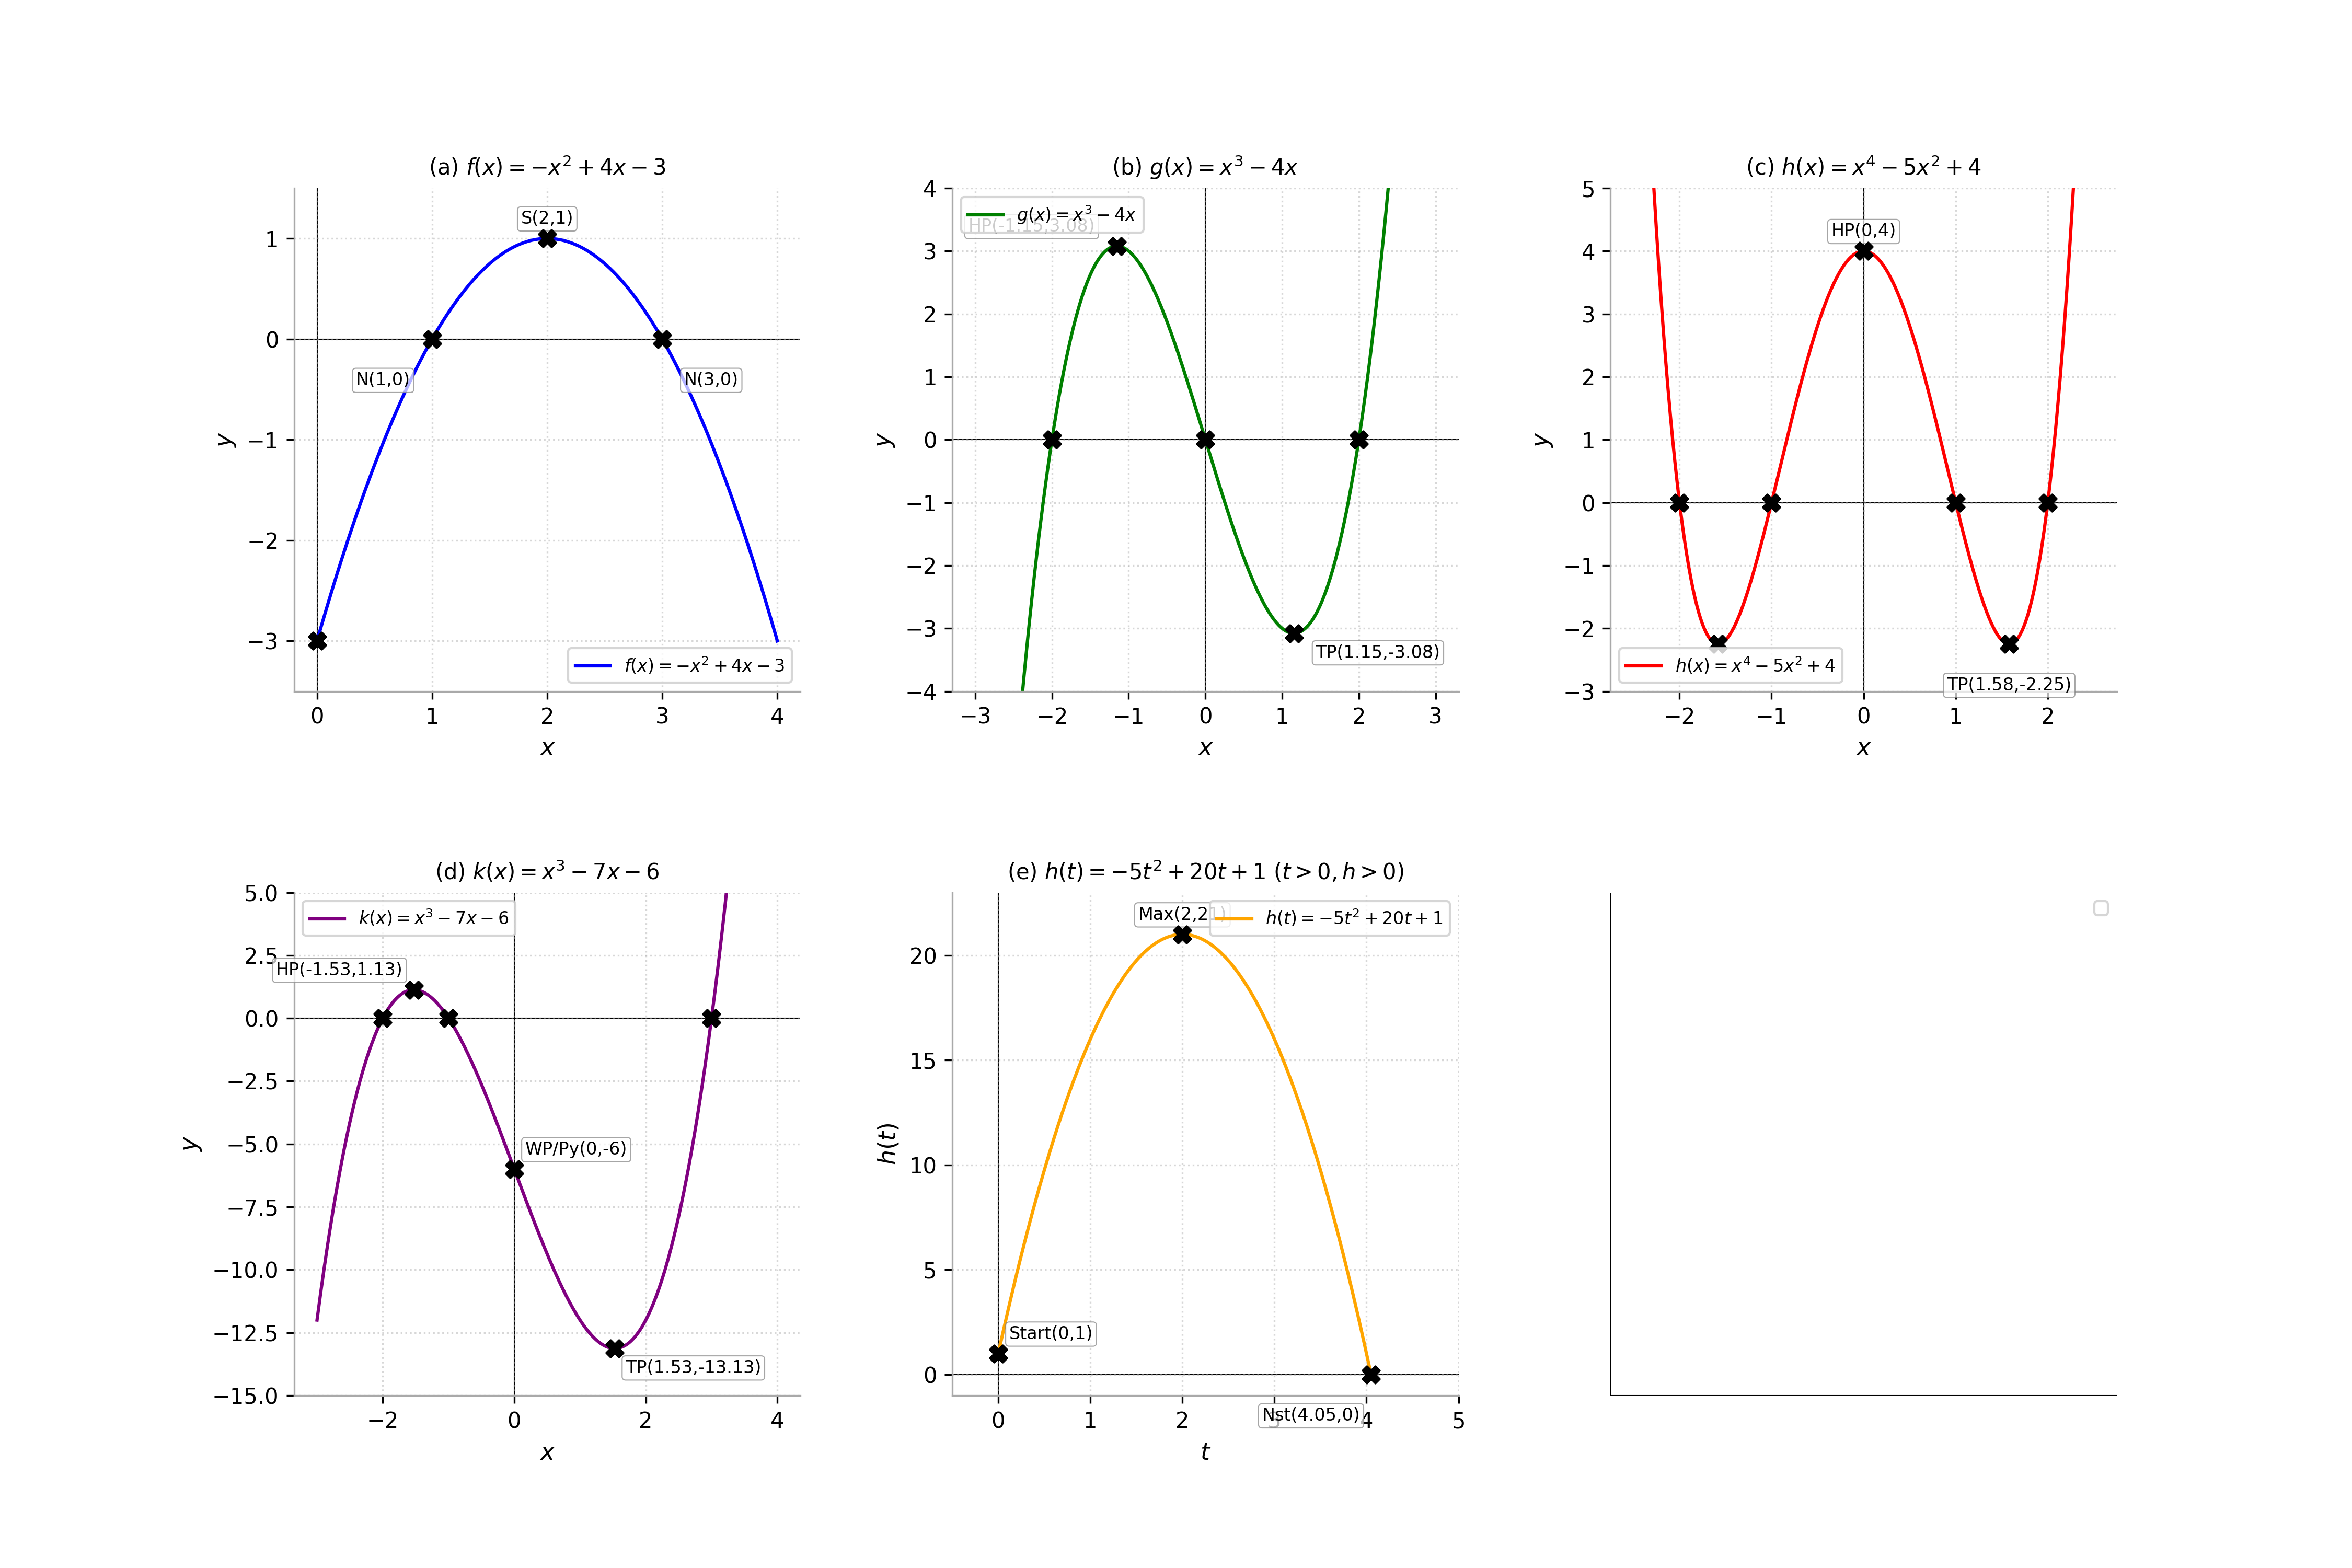
\includegraphics[width=0.8\textwidth]{grafiken/kurvendiskussionen_alle_graphen.png}
    \captionof{figure}{Graphen der untersuchten Funktionen: (a) $f(x)$, (b) $g(x)$, (c) $h(x)$, (d) $k(x)$, und (e) $h(t)$.}
    \label{fig:kurvendisk_alle_graphen}
\end{center}
\end{loesungsumgebung}



\begin{aufgabenumgebung}{Nullstellen aus faktorisierter Form bestimmen}
Bestimme die Nullstellen der folgenden Funktionen. Gib auch an, ob es sich um einfache oder mehrfache Nullstellen handelt. Eine Kurvendiskussion zu diesen Funktionen kann natürlich auch nie schaden.
\begin{enumerate}
    \item $f(x) = (x+4)(x-2.5)(x+1)$
    \item $g(x) = -3x^2(x-1)(x+2)^3$
    \item $h(x) = (x^2-9)(x+1)$ (Tipp: $x^2-9$ weiter faktorisieren!)
    \item $k(x) = 2x^4 - 8x^2$ (Tipp: Erst ausklammern, dann weiter überlegen.)
\end{enumerate}
\end{aufgabenumgebung}

\begin{loesungsumgebung}[loes:nullstellen-faktorisierte-form-wiederholung]{Nullstellen aus faktorisierter Form bestimmen}
Wir bestimmen die Nullstellen der gegebenen Funktionen, indem wir jeden Faktor gleich Null setzen (Satz vom Nullprodukt) und die Vielfachheit der Nullstelle anhand des Exponenten des jeweiligen Linearfaktors bestimmen.

\begin{enumerate}[label=(\alph*)]
    \item \textbf{Funktion $f(x) = (x+4)(x-2.5)(x+1)$} \\
    Setze $f(x)=0$: $(x+4)(x-2.5)(x+1) = 0$.
    \begin{itemize}
        \item $x+4 = 0 \Rightarrow x_1 = -4$. Dies ist eine \textbf{einfache} Nullstelle (Exponent 1).
        \item $x-2.5 = 0 \Rightarrow x_2 = 2.5$. Dies ist eine \textbf{einfache} Nullstelle (Exponent 1).
        \item $x+1 = 0 \Rightarrow x_3 = -1$. Dies ist eine \textbf{einfache} Nullstelle (Exponent 1).
    \end{itemize}
    Die Nullstellen sind $\mathbf{-4}$ (einfach), $\mathbf{2.5}$ (einfach) und $\mathbf{-1}$ (einfach).

    \item \textbf{Funktion $g(x) = -3x^2(x-1)(x+2)^3$} \\
    Setze $g(x)=0$: $-3x^2(x-1)(x+2)^3 = 0$.
    \begin{itemize}
        \item $-3x^2 = 0 \Rightarrow x^2 = 0 \Rightarrow x_1 = 0$. Da der Faktor $x$ mit dem Exponenten 2 auftritt ($x^2$), ist dies eine \textbf{doppelte} Nullstelle.
        \item $x-1 = 0 \Rightarrow x_2 = 1$. Dies ist eine \textbf{einfache} Nullstelle (Exponent 1).
        \item $(x+2)^3 = 0 \Rightarrow x+2 = 0 \Rightarrow x_3 = -2$. Da der Faktor $(x+2)$ mit dem Exponenten 3 auftritt, ist dies eine \textbf{dreifache} Nullstelle.
    \end{itemize}
    Die Nullstellen sind $\mathbf{0}$ (doppelt), $\mathbf{1}$ (einfach) und $\mathbf{-2}$ (dreifach).

    \item \textbf{Funktion $h(x) = (x^2-9)(x+1)$} \\
    Tipp: $x^2-9$ weiter faktorisieren. Mit der 3. binomischen Formel ist $x^2-9 = (x-3)(x+3)$.
    Somit ist $h(x) = (x-3)(x+3)(x+1)$.
    Setze $h(x)=0$: $(x-3)(x+3)(x+1) = 0$.
    \begin{itemize}
        \item $x-3 = 0 \Rightarrow x_1 = 3$. Dies ist eine \textbf{einfache} Nullstelle.
        \item $x+3 = 0 \Rightarrow x_2 = -3$. Dies ist eine \textbf{einfache} Nullstelle.
        \item $x+1 = 0 \Rightarrow x_3 = -1$. Dies ist eine \textbf{einfache} Nullstelle.
    \end{itemize}
    Die Nullstellen sind $\mathbf{3}$ (einfach), $\mathbf{-3}$ (einfach) und $\mathbf{-1}$ (einfach).

    \item \textbf{Funktion $k(x) = 2x^4 - 8x^2$} \\
    Tipp: Erst ausklammern.
    $k(x) = 2x^2(x^2-4)$.
    Den Term $x^2-4$ können wir weiter faktorisieren: $x^2-4 = (x-2)(x+2)$.
    Somit ist $k(x) = 2x^2(x-2)(x+2)$.
    Setze $k(x)=0$: $2x^2(x-2)(x+2) = 0$.
    \begin{itemize}
        \item $2x^2 = 0 \Rightarrow x^2=0 \Rightarrow x_1 = 0$. Dies ist eine \textbf{doppelte} Nullstelle (wegen $x^2$).
        \item $x-2 = 0 \Rightarrow x_2 = 2$. Dies ist eine \textbf{einfache} Nullstelle.
        \item $x+2 = 0 \Rightarrow x_3 = -2$. Dies ist eine \textbf{einfache} Nullstelle.
    \end{itemize}
    Die Nullstellen sind $\mathbf{0}$ (doppelt), $\mathbf{2}$ (einfach) und $\mathbf{-2}$ (einfach).
\end{enumerate}
Eine vollständige Kurvendiskussion würde zusätzlich Symmetrie, Verhalten im Unendlichen, Extrempunkte, Wendepunkte und das Krümmungsverhalten untersuchen. Die Kenntnis der Nullstellen und ihrer Vielfachheit ist dabei ein wichtiger erster Schritt, da sie Aufschluss über das Verhalten des Graphen an der x-Achse gibt (Schneiden bei einfacher/ungerader Vielfachheit, Berühren bei doppelter/gerader Vielfachheit).
\end{loesungsumgebung}



\begin{aufgabenumgebung}{Grenzwerte und Symmetrie gebrochen-rationaler Grundfunktionen}
\begin{enumerate}
    \item Bestimme den Definitionsbereich und das Verhalten für $x \to 0^+$ und $x \to 0^-$ für die folgenden Funktionen. Gib auch an, ob es sich um eine Polstelle mit oder ohne Vorzeichenwechsel handelt.
        \begin{itemize}
            \item $f_1(x) = \frac{3}{x^3}$
            \item $f_2(x) = -\frac{1}{x^4}$
            \item $f_3(x) = \frac{10}{x}$
        \end{itemize}
    \item Untersuche die Symmetrie der Funktionen aus Teilaufgabe 1 (Achsensymmetrie zur y-Achse oder Punktsymmetrie zum Ursprung).
    \item \textbf{Zuordnung Aufgabe:} Ordne den folgenden Funktionsgraphen $k_1(x) = \frac{1}{x^2}$, $k_2(x) = -\frac{1}{x}$, $k_3(x) = \frac{2}{x^3}$, $k_4(x) = \frac{1}{x^4}$ die passenden Funktionsgleichungen zu. Begründe deine Entscheidung anhand des Verhaltens an der Polstelle $x=0$ und der Symmetrie.
    \begin{center}
        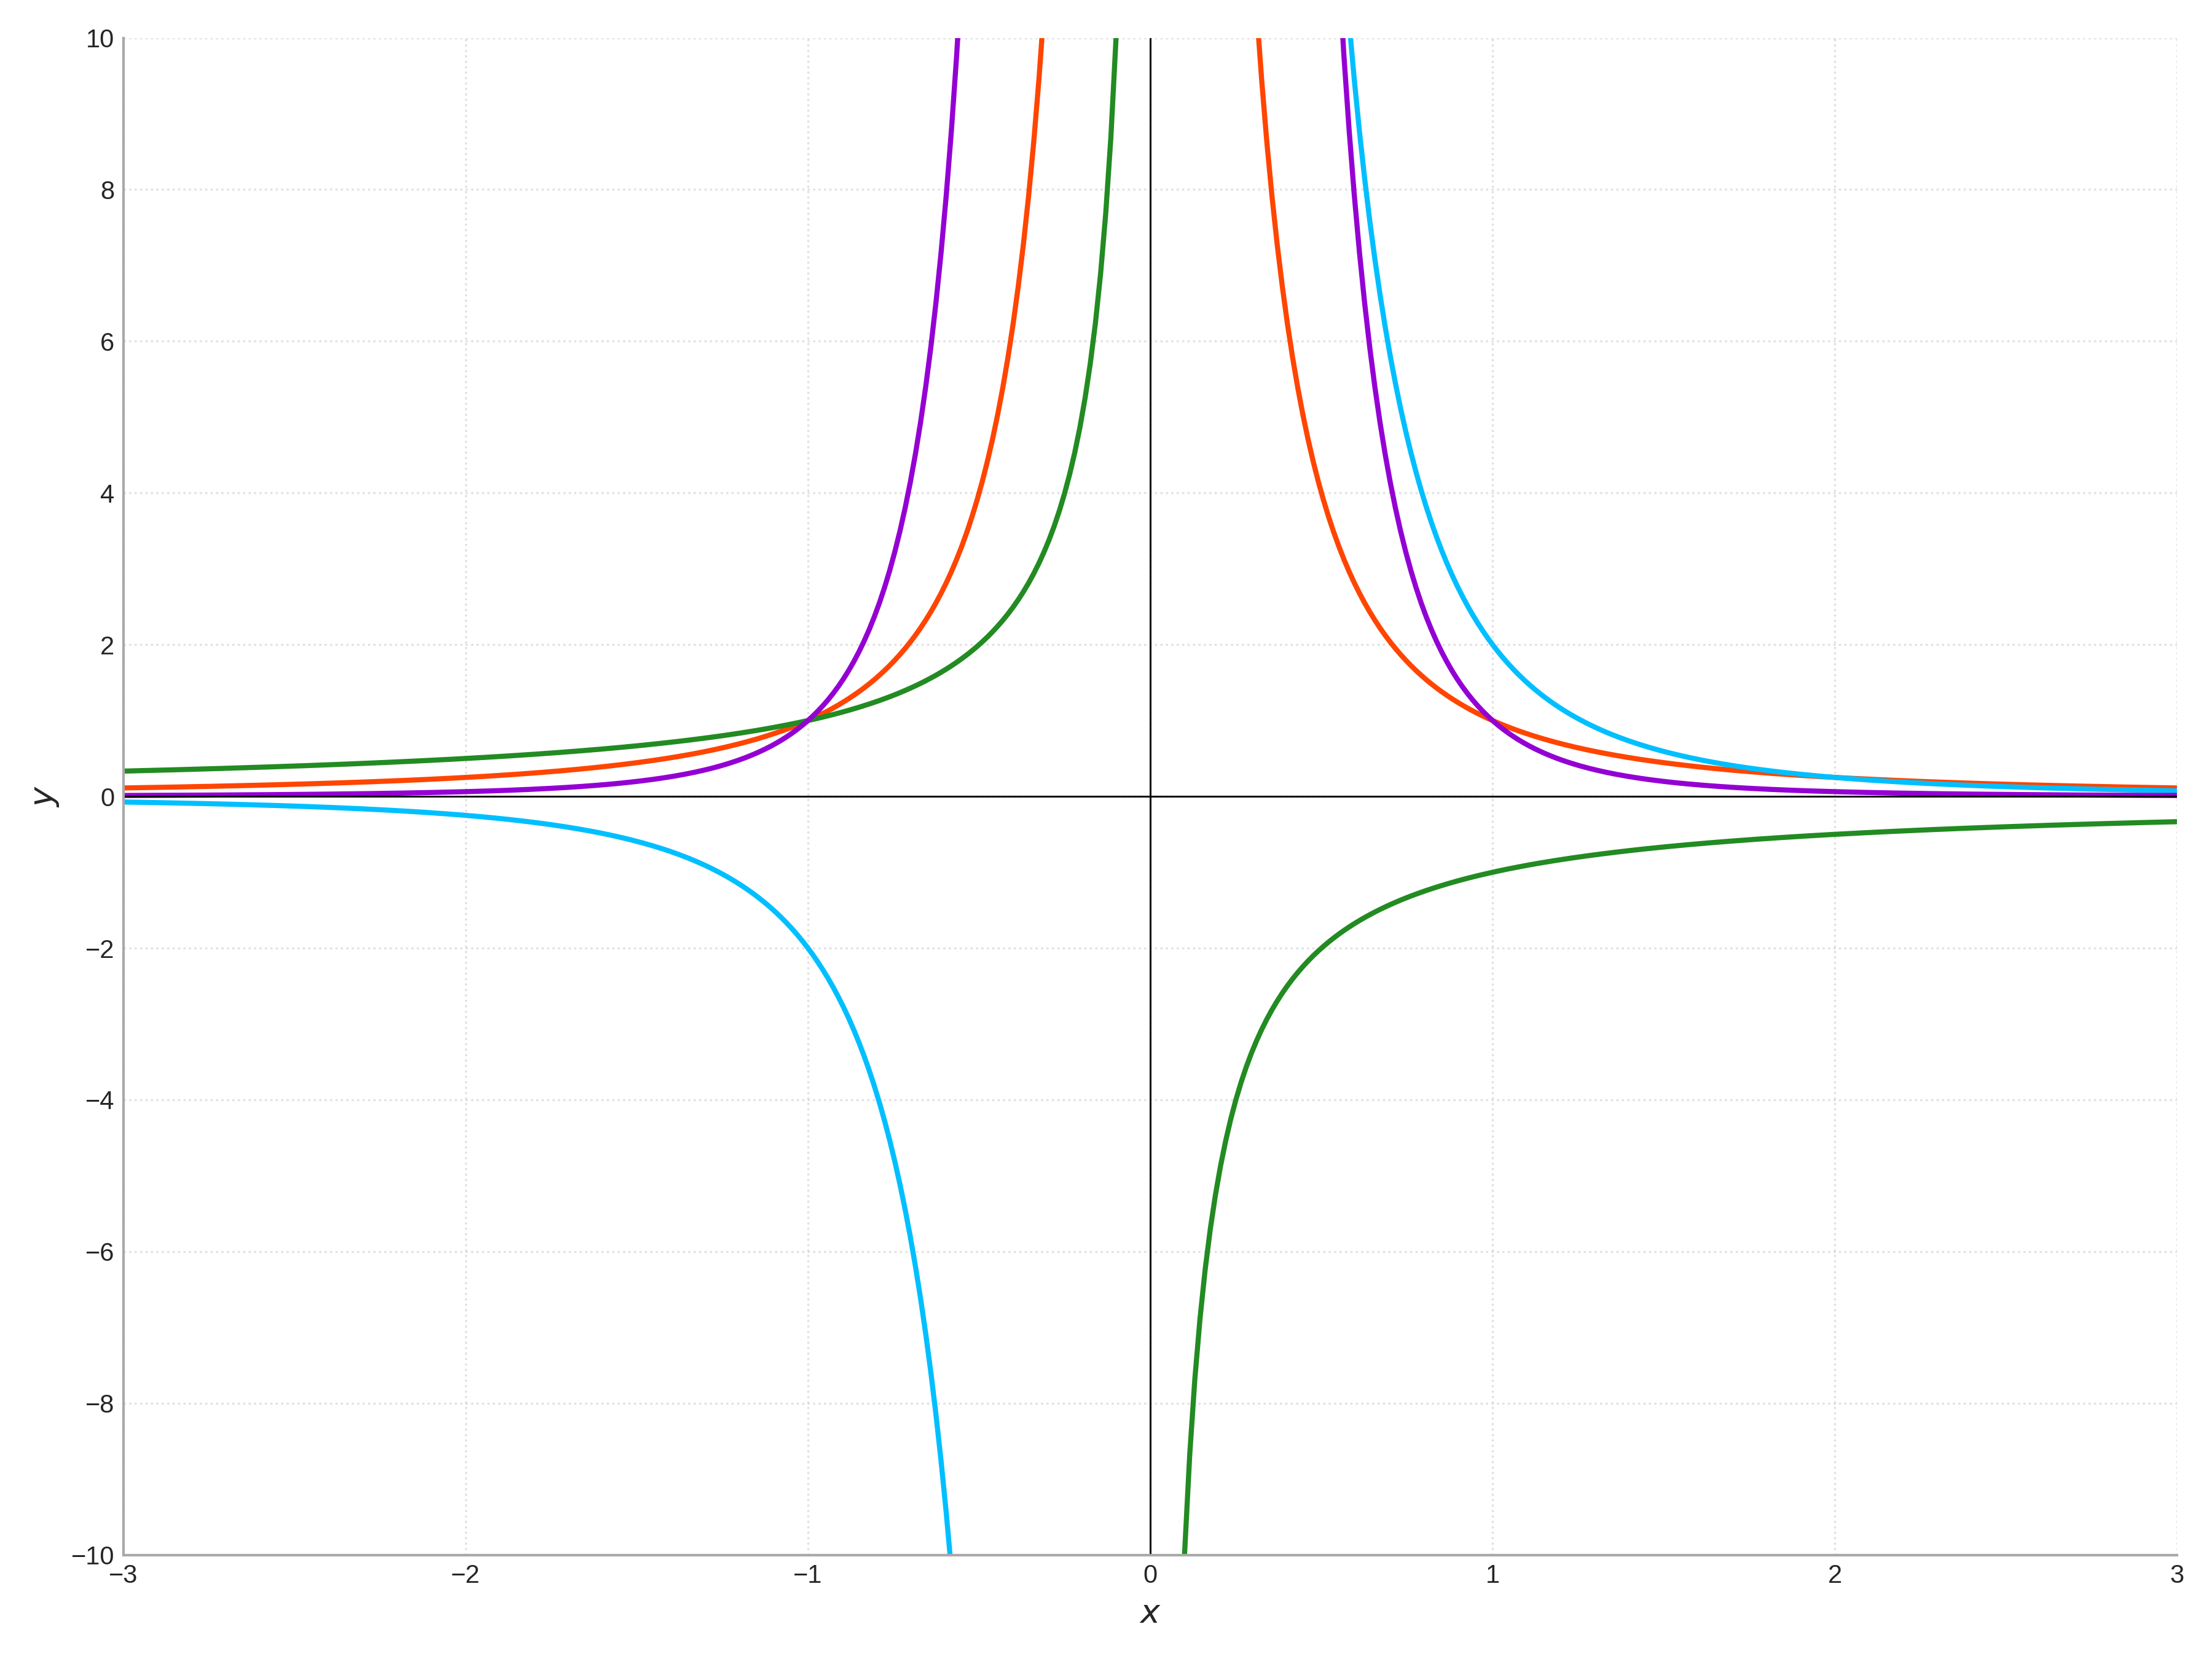
\includegraphics[width=0.9\textwidth]{grafiken/Zuordnung_Polstellen.png}
        \captionof{figure}{Graphen zur Zuordnung von Polstellenverhalten}
        \label{fig:zuordnung_polstellen}
    \end{center}
\end{enumerate}
\end{aufgabenumgebung}

\begin{loesungsumgebung}[loes:grenzwerte-symmetrie-gebrochen-rational]{Grenzwerte und Symmetrie gebrochen-rationaler Grundfunktionen}

\begin{enumerate}[label=(\alph*)]
    \item \textbf{Definitionsbereich und Verhalten für $x \to 0^\pm$}
    \begin{itemize}
        \item \textbf{Funktion $f_1(x) = \frac{3}{x^3}$}
        \begin{itemize}
            \item Definitionsbereich: $D_{f1} = \mathbb{R} \setminus \{0\}$.
            \item Verhalten an der Polstelle $x=0$:
            Für $x \to 0^+$: $x^3 \to 0^+$ (kleine positive Werte) $\implies f_1(x) = \frac{3}{x^3} \to +\infty$.
            Für $x \to 0^-$: $x^3 \to 0^-$ (kleine negative Werte) $\implies f_1(x) = \frac{3}{x^3} \to -\infty$.
            \item Es handelt sich um eine \textbf{Polstelle mit Vorzeichenwechsel} (VZW), da der Exponent im Nenner (3) ungerade ist.
        \end{itemize}

        \item \textbf{Funktion $f_2(x) = -\frac{1}{x^4}$}
        \begin{itemize}
            \item Definitionsbereich: $D_{f2} = \mathbb{R} \setminus \{0\}$.
            \item Verhalten an der Polstelle $x=0$:
            Für $x \to 0^+$: $x^4 \to 0^+$ $\implies f_2(x) = -\frac{1}{x^4} \to -\infty$.
            Für $x \to 0^-$: $x^4 \to 0^+$ $\implies f_2(x) = -\frac{1}{x^4} \to -\infty$.
            \item Es handelt sich um eine \textbf{Polstelle ohne Vorzeichenwechsel} (OVZW), da der Exponent im Nenner (4) gerade ist. Beide Äste gehen gegen $-\infty$.
        \end{itemize}

        \item \textbf{Funktion $f_3(x) = \frac{10}{x}$}
        \begin{itemize}
            \item Definitionsbereich: $D_{f3} = \mathbb{R} \setminus \{0\}$.
            \item Verhalten an der Polstelle $x=0$:
            Für $x \to 0^+$: $x \to 0^+$ $\implies f_3(x) = \frac{10}{x} \to +\infty$.
            Für $x \to 0^-$: $x \to 0^-$ $\implies f_3(x) = \frac{10}{x} \to -\infty$.
            \item Es handelt sich um eine \textbf{Polstelle mit Vorzeichenwechsel} (VZW), da der Exponent im Nenner (1) ungerade ist.
        \end{itemize}
    \end{itemize}

    \item \textbf{Symmetrieuntersuchung der Funktionen aus Teilaufgabe 1}
    \begin{itemize}
        \item \textbf{Funktion $f_1(x) = \frac{3}{x^3}$}
        $f_1(-x) = \frac{3}{(-x)^3} = \frac{3}{-x^3} = -\frac{3}{x^3} = -f_1(x)$.
        Die Funktion $f_1(x)$ ist \textbf{punktsymmetrisch zum Ursprung}.

        \item \textbf{Funktion $f_2(x) = -\frac{1}{x^4}$}
        $f_2(-x) = -\frac{1}{(-x)^4} = -\frac{1}{x^4} = f_2(x)$.
        Die Funktion $f_2(x)$ ist \textbf{achsensymmetrisch zur y-Achse}.

        \item \textbf{Funktion $f_3(x) = \frac{10}{x}$}
        $f_3(-x) = \frac{10}{(-x)} = -\frac{10}{x} = -f_3(x)$.
        Die Funktion $f_3(x)$ ist \textbf{punktsymmetrisch zum Ursprung}.
    \end{itemize}

    \item \textbf{Zuordnung Aufgabe:}
    Wir analysieren die gegebenen Funktionen $k_1(x) = \frac{1}{x^2}$, $k_2(x) = -\frac{1}{x}$, $k_3(x) = \frac{2}{x^3}$, $k_4(x) = \frac{1}{x^4}$ und ordnen sie den Graphen in der Abbildung zu (die Farben beziehen sich auf die typische Darstellung solcher Graphen in der von Ihnen hochgeladenen Abbildung).

    \begin{itemize}
        \item \textbf{$k_1(x) = \frac{1}{x^2}$:}
        \begin{itemize}
            \item Verhalten bei $x=0$: Polstelle ohne Vorzeichenwechsel. $\lim_{x \to 0^\pm} k_1(x) = +\infty$. (Beide Äste gehen nach oben).
            \item Symmetrie: $k_1(-x) = \frac{1}{(-x)^2} = \frac{1}{x^2} = k_1(x) \implies$ Achsensymmetrisch zur y-Achse.
            \item Werte: $k_1(x) > 0$ für alle $x \neq 0$. $k_1(1)=1, k_1(2)=0.25$.
        \end{itemize}
        \textit{Mathematische Begründung für Zuordnung:} Dieser Graph muss achsensymmetrisch sein und sich für $x \to 0$ nach $+\infty$ entwickeln.
        In der typischen Darstellung (Abbildung 5.10) ist dies der \textbf{orange Graph}. Er ist achsensymmetrisch und beide Äste streben gegen $+\infty$.

        \item \textbf{$k_2(x) = -\frac{1}{x}$:}
        \begin{itemize}
            \item Verhalten bei $x=0$: Polstelle mit Vorzeichenwechsel. $\lim_{x \to 0^+} k_2(x) = -\infty$, $\lim_{x \to 0^-} k_2(x) = +\infty$.
            \item Symmetrie: $k_2(-x) = -\frac{1}{-x} = \frac{1}{x} = -(-\frac{1}{x}) = -k_2(x) \implies$ Punktsymmetrisch zum Ursprung.
            \item Werte: Für $x>0$ ist $k_2(x)<0$ (IV. Quadrant). Für $x<0$ ist $k_2(x)>0$ (II. Quadrant).
        \end{itemize}
        \textit{Mathematische Begründung für Zuordnung:} Dieser Graph muss punktsymmetrisch sein, wobei der rechte Ast ($x>0$) nach $-\infty$ und der linke Ast ($x<0$) nach $+\infty$ strebt.
        In der typischen Darstellung (Abbildung 5.10) ist dies der \textbf{hellblaue (cyan) Graph}.

        \item \textbf{$k_3(x) = \frac{2}{x^3}$:}
        \begin{itemize}
            \item Verhalten bei $x=0$: Polstelle mit Vorzeichenwechsel. $\lim_{x \to 0^+} k_3(x) = +\infty$, $\lim_{x \to 0^-} k_3(x) = -\infty$.
            \item Symmetrie: $k_3(-x) = \frac{2}{(-x)^3} = -\frac{2}{x^3} = -k_3(x) \implies$ Punktsymmetrisch zum Ursprung.
            \item Werte: Für $x>0$ ist $k_3(x)>0$ (I. Quadrant). Für $x<0$ ist $k_3(x)<0$ (III. Quadrant). Der Faktor 2 im Zähler bewirkt eine Streckung im Vergleich zu $1/x^3$.
        \end{itemize}
        \textit{Mathematische Begründung für Zuordnung:} Dieser Graph muss punktsymmetrisch sein, wobei der rechte Ast ($x>0$) nach $+\infty$ und der linke Ast ($x<0$) nach $-\infty$ strebt.
        In der typischen Darstellung (Abbildung 5.10) ist dies der \textbf{grüne Graph}.

        \item \textbf{$k_4(x) = \frac{1}{x^4}$:}
        \begin{itemize}
            \item Verhalten bei $x=0$: Polstelle ohne Vorzeichenwechsel. $\lim_{x \to 0^\pm} k_4(x) = +\infty$. (Beide Äste gehen nach oben).
            \item Symmetrie: $k_4(-x) = \frac{1}{(-x)^4} = \frac{1}{x^4} = k_4(x) \implies$ Achsensymmetrisch zur y-Achse.
            \item Werte: $k_4(x) > 0$ für alle $x \neq 0$. Im Vergleich zu $k_1(x)=1/x^2$: Für $|x|<1$ ist $x^4 < x^2 \implies 1/x^4 > 1/x^2$ (steilerer Anstieg gegen Pol). Für $|x|>1$ ist $x^4 > x^2 \implies 1/x^4 < 1/x^2$ (schnellere Annäherung an die x-Achse).
        \end{itemize}
        \textit{Mathematische Begründung für Zuordnung:} Dieser Graph muss achsensymmetrisch sein, sich für $x \to 0$ nach $+\infty$ entwickeln und im Vergleich zu $1/x^2$ steiler an der Polstelle sein und sich schneller der x-Achse annähern.
        In der typischen Darstellung (Abbildung 5.10) ist dies der \textbf{lila (purple) Graph}. Er ist achsensymmetrisch, beide Äste streben gegen $+\infty$ und er ist 'enger' an der y-Achse und flacher für größere $|x|$ im Vergleich zum orangen Graphen.
    \end{itemize}
    \textbf{Zusammenfassende Zuordnung (basierend auf typischer Farbgebung der Abbildung 5.10):}
    \begin{itemize}
        \item Orange Kurve: $k_1(x) = \frac{1}{x^2}$
        \item Hellblaue (Cyan) Kurve: $k_2(x) = -\frac{1}{x}$
        \item Grüne Kurve: $k_3(x) = \frac{2}{x^3}$
        \item Lila (Purple) Kurve: $k_4(x) = \frac{1}{x^4}$
    \end{itemize}
\end{enumerate}

\end{loesungsumgebung}


\begin{aufgabenumgebung}{Funktionen mit negativen Exponenten und Substitution}
\begin{enumerate}
    \item Bestimme für die folgenden Funktionen den Definitionsbereich, die Gleichung der senkrechten Asymptote(n) und das Verhalten der Funktion für $x$ gegen die Polstelle(n) (einseitige Grenzwerte) sowie für $x \to \pm\infty$. Untersuche auch das Symmetrieverhalten bezüglich der senkrechten Asymptote oder eines Punktes.
        \begin{itemize}
            \item $f_1(x) = \frac{-1}{x+2}$
            \item $f_2(x) = \frac{3}{(x-3)^2}$
            \item $f_3(x) = 1 - \frac{1}{x^2}$ (Tipp: Was ist hier die horizontale Asymptote?)
        \end{itemize}
    \item Skizziere die Graphen der Funktionen aus Teilaufgabe 1.
    \item \textbf{Transformationskette verstehen:}
        Beschreibe, wie der Graph der Funktion $g(x) = \frac{-2}{(x+3)^2} - 4$ aus dem Graphen der Grundfunktion $h(u) = \frac{1}{u^2}$ durch Streckung/Stauchung, Spiegelung und Verschiebungen hervorgeht. Gib den Definitionsbereich und die Gleichungen der Asymptoten von $g(x)$ an.
\end{enumerate}
\end{aufgabenumgebung}

\begin{loesungsumgebung}[loes:funktionen-neg-exponent-substitution]{Funktionen mit negativen Exponenten und Substitution}

\begin{enumerate}[label=(\alph*)]
    \item \textbf{Untersuchung der Funktionen $f_1(x), f_2(x), f_3(x)$}
    \begin{itemize}
        \item \textbf{Funktion $f_1(x) = \frac{-1}{x+2}$}
        \begin{itemize}
            \item \textit{Definitionsbereich:} Der Nenner $x+2$ darf nicht Null sein, also $x \neq -2$. $D_{f1} = \mathbb{R} \setminus \{-2\}$.
            \item \textit{Senkrechte Asymptote:} Bei $x=-2$ liegt eine Polstelle vor. Die Gleichung der senkrechten Asymptote ist $\mathbf{x=-2}$.
            \item \textit{Verhalten an der Polstelle $x=-2$:}
            Für $x \to -2^+$ (z.B. $x=-1.9$, $x+2$ ist klein und positiv): $f_1(x) = \frac{-1}{\text{klein pos.}} \to -\infty$.
            Für $x \to -2^-$ (z.B. $x=-2.1$, $x+2$ ist klein und negativ): $f_1(x) = \frac{-1}{\text{klein neg.}} \to +\infty$.
            Es handelt sich um eine Polstelle mit Vorzeichenwechsel.
            \item \textit{Verhalten für $x \to \pm\infty$:}
            $\lim_{x \to \pm\infty} \frac{-1}{x+2} = \lim_{x \to \pm\infty} \frac{-1/x}{1+2/x} = \frac{0}{1} = 0$.
            Die horizontale Asymptote ist $\mathbf{y=0}$.
            \item \textit{Symmetrie:} Der Graph von $f_1(x)$ ist punktsymmetrisch zum Schnittpunkt seiner Asymptoten, dem Punkt $\mathbf{(-2|0)}$. (Verschobene Hyperbel $y' = -1/x'$ um $(-2,0)$).
        \end{itemize}

        \item \textbf{Funktion $f_2(x) = \frac{3}{(x-3)^2}$}
        \begin{itemize}
            \item \textit{Definitionsbereich:} Der Nenner $(x-3)^2$ darf nicht Null sein, also $x \neq 3$. $D_{f2} = \mathbb{R} \setminus \{3\}$.
            \item \textit{Senkrechte Asymptote:} Bei $x=3$ liegt eine Polstelle vor. Die Gleichung der senkrechten Asymptote ist $\mathbf{x=3}$.
            \item \textit{Verhalten an der Polstelle $x=3$:}
            Der Nenner $(x-3)^2$ ist für $x \neq 3$ immer positiv und geht gegen $0^+$ für $x \to 3^\pm$.
            Für $x \to 3^+$: $f_2(x) = \frac{3}{(x-3)^2} \to \frac{3}{\text{klein pos.}} \to +\infty$.
            Für $x \to 3^-$: $f_2(x) = \frac{3}{(x-3)^2} \to \frac{3}{\text{klein pos.}} \to +\infty$.
            Es handelt sich um eine Polstelle ohne Vorzeichenwechsel.
            \item \textit{Verhalten für $x \to \pm\infty$:}
            $\lim_{x \to \pm\infty} \frac{3}{(x-3)^2} = 0$.
            Die horizontale Asymptote ist $\mathbf{y=0}$.
            \item \textit{Symmetrie:} Der Graph von $f_2(x)$ ist achsensymmetrisch zur senkrechten Asymptote $\mathbf{x=3}$. (Verschobene und gestreckte Funktion $y' = 1/(x')^2$).
        \end{itemize}

        \item \textbf{Funktion $f_3(x) = 1 - \frac{1}{x^2}$}
        \begin{itemize}
            \item \textit{Definitionsbereich:} Der Nenner $x^2$ darf nicht Null sein, also $x \neq 0$. $D_{f3} = \mathbb{R} \setminus \{0\}$.
            \item \textit{Senkrechte Asymptote:} Bei $x=0$ liegt eine Polstelle vor. Die Gleichung der senkrechten Asymptote ist $\mathbf{x=0}$ (die y-Achse).
            \item \textit{Verhalten an der Polstelle $x=0$:}
            Der Term $x^2$ ist für $x \neq 0$ immer positiv und geht gegen $0^+$ für $x \to 0^\pm$.
            Somit $\frac{1}{x^2} \to +\infty$ für $x \to 0^\pm$.
            Daher $f_3(x) = 1 - \frac{1}{x^2} \to 1 - (+\infty) \to -\infty$ für $x \to 0^\pm$.
            Es handelt sich um eine Polstelle ohne Vorzeichenwechsel (für den gebrochen-rationalen Anteil, beide Äste von $f_3(x)$ gehen gegen $-\infty$).
            \item \textit{Verhalten für $x \to \pm\infty$:}
            $\lim_{x \to \pm\infty} \frac{1}{x^2} = 0$.
            $\lim_{x \to \pm\infty} \left(1 - \frac{1}{x^2}\right) = 1 - 0 = 1$.
            Die horizontale Asymptote ist $\mathbf{y=1}$.
            \item \textit{Symmetrie:} $f_3(-x) = 1 - \frac{1}{(-x)^2} = 1 - \frac{1}{x^2} = f_3(x)$.
            Der Graph von $f_3(x)$ ist \textbf{achsensymmetrisch zur y-Achse} (welche die senkrechte Asymptote ist).
        \end{itemize}
    \end{itemize}

    \item \textbf{Skizze der Graphen aus Teilaufgabe 1} \\
    Die Graphen werden in einem gemeinsamen Koordinatensystem skizziert, wobei die jeweiligen Asymptoten und das Verhalten an den Polstellen sowie im Unendlichen berücksichtigt werden.
    \begin{center}
    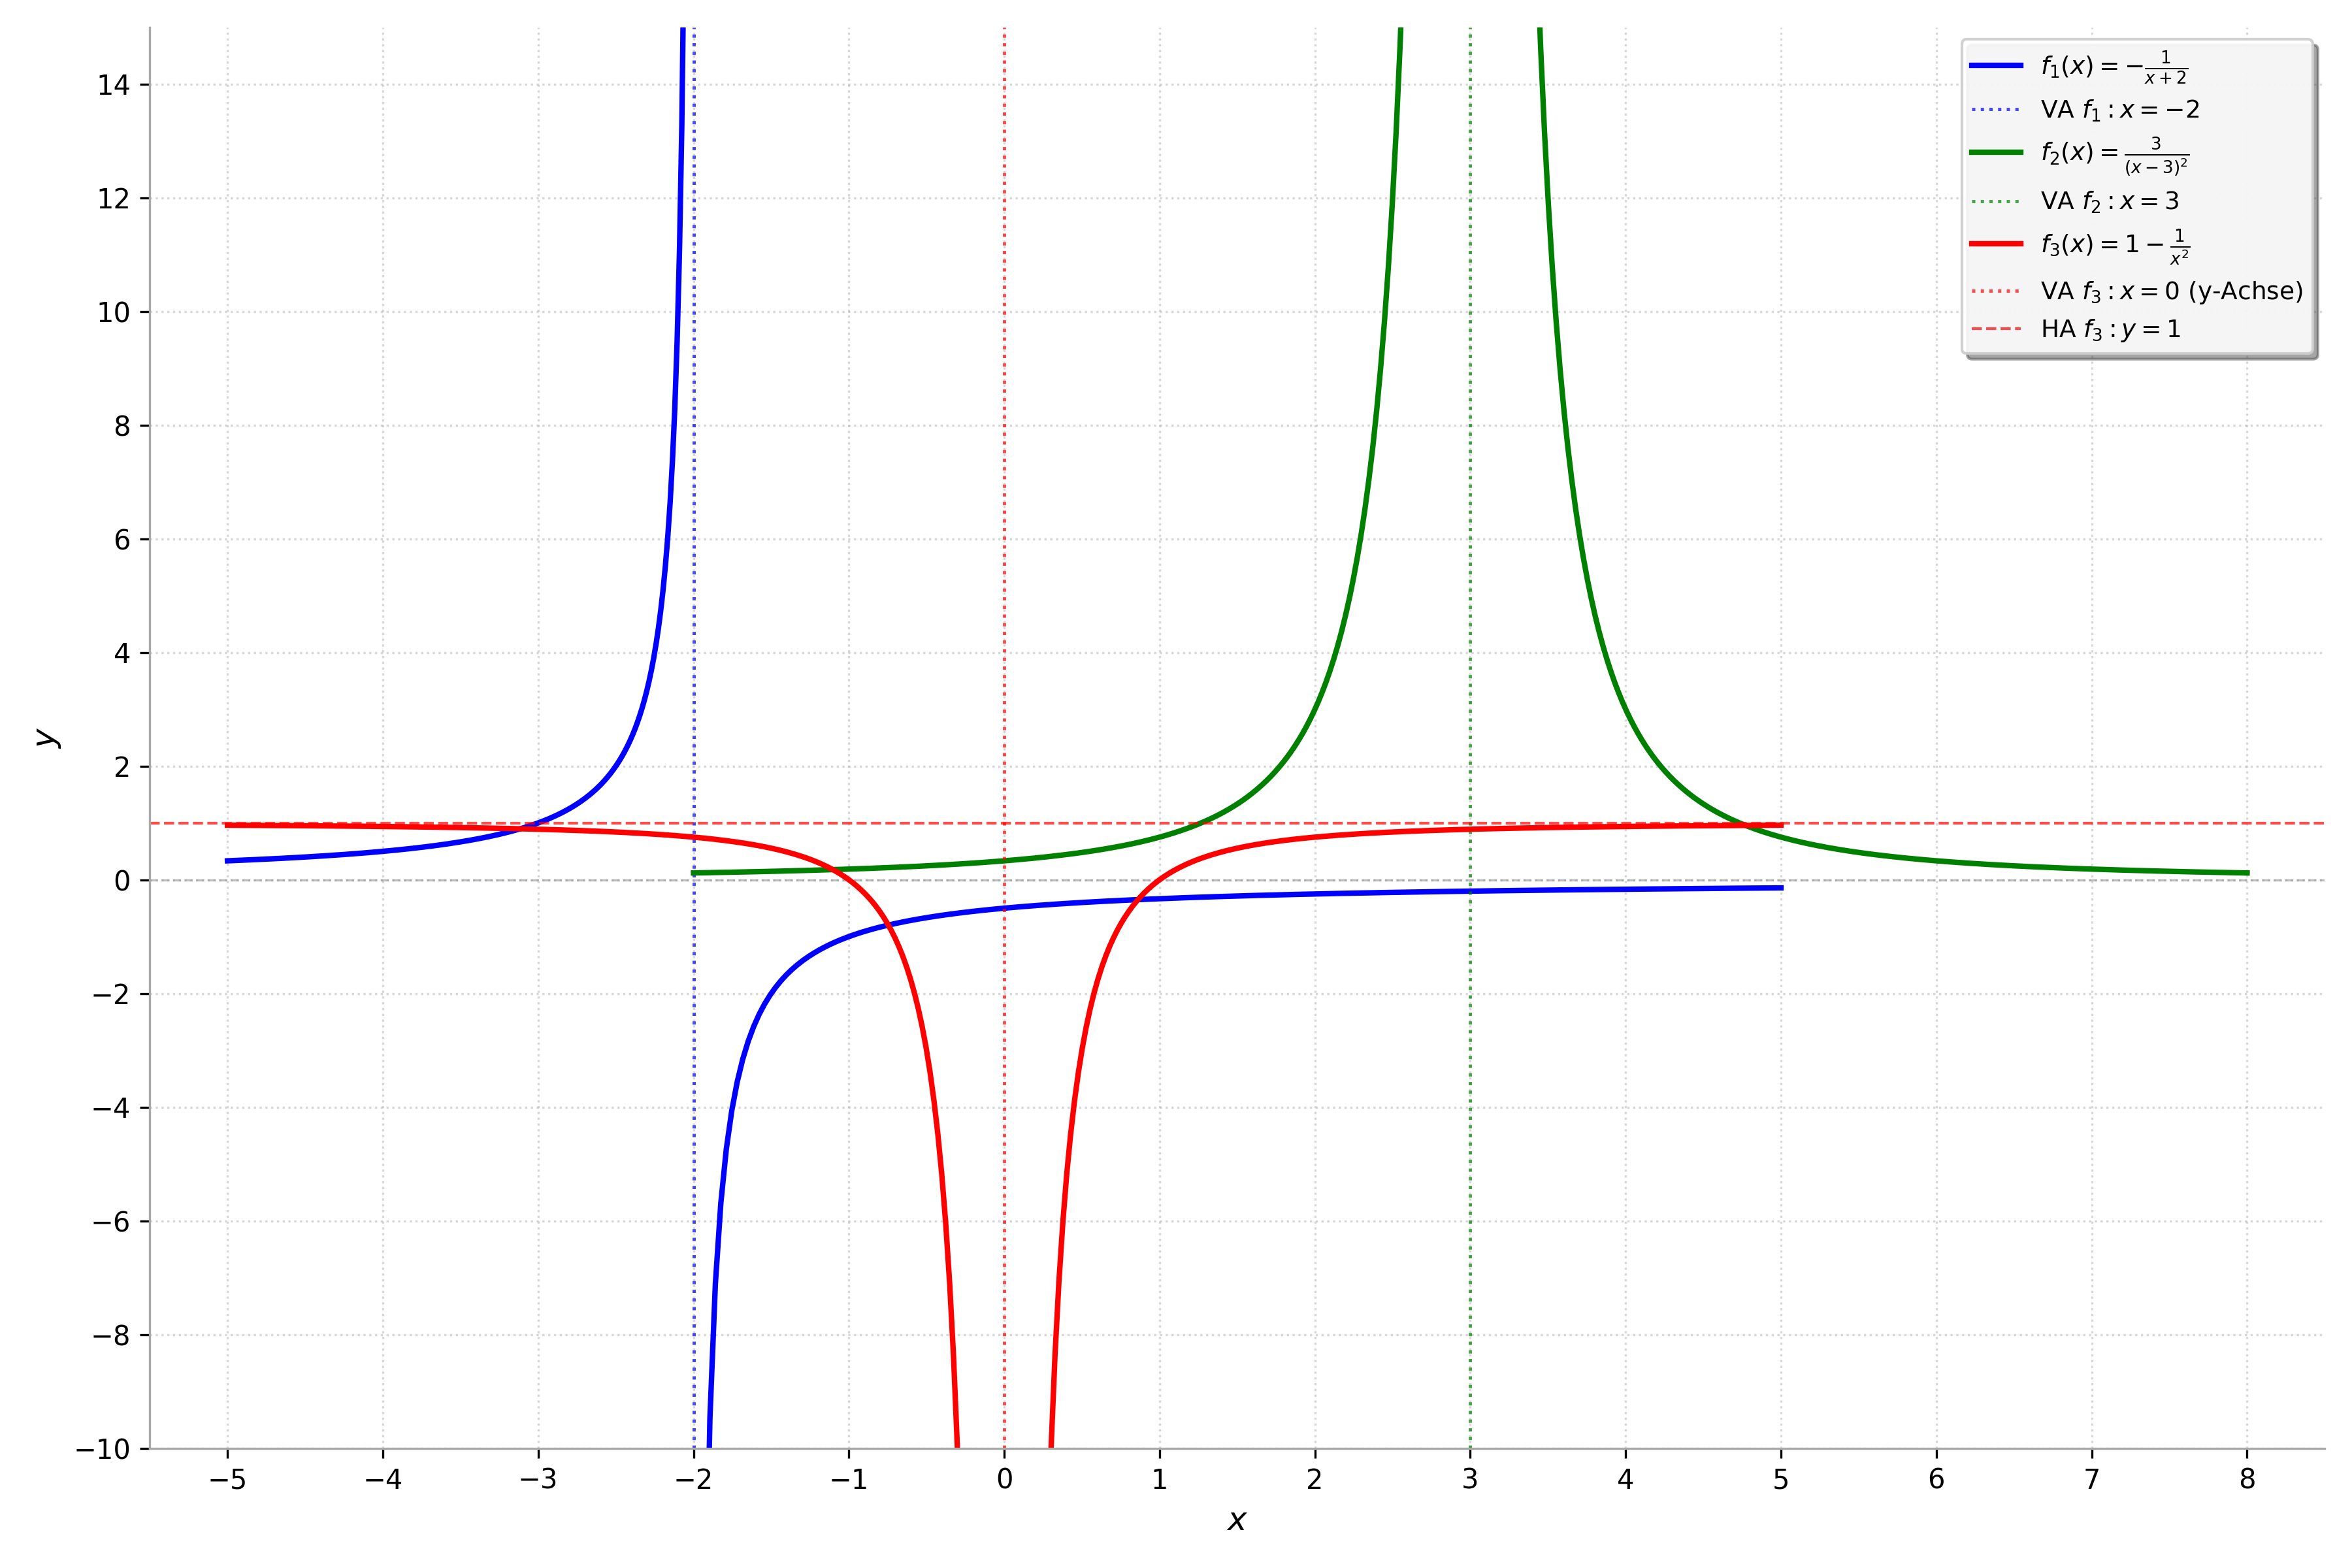
\includegraphics[width=0.8\textwidth]{grafiken/funktionen_neg_exp_kombi_graph.png}
    % --- Beschreibung der Grafik ---
    % Die Grafik zeigt ein Koordinatensystem mit drei Graphen:
    % 1. f1(x) = -1/(x+2): VA bei x=-2, HA bei y=0. Hyperbelähnliche Äste im II. und IV. Quadranten relativ zum Asymptotenkreuz (-2|0). Für x -> -2+ geht f1 -> -unendlich, für x -> -2- geht f1 -> +unendlich.
    % 2. f2(x) = 3/((x-3)^2): VA bei x=3, HA bei y=0. Beide Äste gehen für x -> 3 gegen +unendlich. Symmetrisch zu x=3.
    % 3. f3(x) = 1 - 1/x^2: VA bei x=0 (y-Achse), HA bei y=1. Beide Äste gehen für x -> 0 gegen -unendlich. Symmetrisch zur y-Achse. Der Graph nähert sich von unten der Asymptote y=1.
    \captionof{figure}{Skizzen der Graphen von $f_1(x)$, $f_2(x)$ und $f_3(x)$ mit ihren Asymptoten.}
    \label{fig:funktionen_neg_exp_kombi_graph}
    \end{center}

    \item \textbf{Transformationskette verstehen: $g(x) = \frac{-2}{(x+3)^2} - 4$ aus $h(u) = \frac{1}{u^2}$}
    Der Graph von $g(x)$ geht aus dem Graphen der Grundfunktion $h(u) = \frac{1}{u^2}$ durch folgende Transformationen hervor:
    \begin{enumerate}
        \item \textbf{Streckung in y-Richtung} mit dem Faktor 2: $h_1(u) = 2 \cdot h(u) = \frac{2}{u^2}$.
        \item \textbf{Spiegelung an der x-Achse:} $h_2(u) = -h_1(u) = -\frac{2}{u^2}$.
        \item \textbf{Verschiebung um 3 Einheiten nach links} in x-Richtung (ersetze $u$ durch $x+3$): $h_3(x) = h_2(x+3) = -\frac{2}{(x+3)^2}$.
        \item \textbf{Verschiebung um 4 Einheiten nach unten} in y-Richtung: $g(x) = h_3(x) - 4 = -\frac{2}{(x+3)^2} - 4$.
    \end{enumerate}
    \textbf{Definitionsbereich von $g(x)$:}
    Der Nenner $(x+3)^2$ darf nicht Null sein, also $x+3 \neq 0 \Rightarrow x \neq -3$.
    $D_g = \mathbb{R} \setminus \{-3\}$.
    \textbf{Gleichungen der Asymptoten von $g(x)$:}
    \begin{itemize}
        \item Die Verschiebung nach links ändert die senkrechte Asymptote von $u=0$ zu $x+3=0$, also $\mathbf{x=-3}$.
        \item Die Streckung und Spiegelung beeinflussen die horizontale Asymptote $y=0$ nicht. Die Verschiebung nach unten um 4 Einheiten verschiebt die horizontale Asymptote zu $\mathbf{y=-4}$.
        ($\lim_{x \to \pm\infty} \left(-\frac{2}{(x+3)^2} - 4\right) = 0 - 4 = -4$).
    \end{itemize}
\end{enumerate}

\end{loesungsumgebung}


\begin{aufgabenumgebung}[A:DiffUebergreifend]{Übergreifende Übungsaufgaben zum bisherigen Kapitel Differentialrechnung}
\begin{enumerate}
    \item \textbf{Polynom-Analyse (Grad 3):}
        Gegeben ist die Funktion $f(x) = -\frac{1}{3}x^3 + x^2 + 3x - \frac{7}{3}$.
        \begin{enumerate}
            \item Führe eine vollständige Kurvendiskussion für $f(x)$ durch (Definitionsbereich, Symmetrie, Verhalten im Unendlichen, Achsenschnittpunkte, Extrempunkte, Wendepunkte, Monotonie, Krümmung).
            \item Zeichne den Graphen von $f(x)$ im Intervall $[-4, 6]$ unter Verwendung deiner Ergebnisse.
            \item Bestimme die Gleichung der Tangente an den Graphen von $f(x)$ im Punkt $P(0|f(0))$.
            \item In welchem Punkt hat die Tangente an den Graphen von $f(x)$ die Steigung $m=-5$?
        \end{enumerate}
    \item \textbf{Optimierungsproblem – Die optimale Dose:}
        Eine zylinderförmige Konservendose soll ein Volumen von $V = 500 \text{ cm}^3$ haben. Die Materialkosten sollen minimiert werden, d.h. die Oberfläche $O$ der Dose soll minimal werden.
        Die Formeln für einen Zylinder mit Radius $r$ und Höhe $h$ sind:
        Volumen: $V = \pi r^2 h$
        Oberfläche (Mantel + 2 Deckel): $O = 2\pi r^2 + 2\pi r h$
        \begin{enumerate}
            \item \textbf{Zielfunktion aufstellen:} Drücke die Oberfläche $O$ als Funktion nur einer Variablen (z.B. des Radius $r$) aus. Nutze dazu die Nebenbedingung für das Volumen $V=500 \text{ cm}^3$, um $h$ durch $r$ auszudrücken und in die Oberflächenformel einzusetzen. Du erhältst $O(r)$.
            \item \textbf{Ableitung bilden:} Bilde die erste Ableitung $O'(r)$. (Hinweis: $O(r)$ wird einen Term der Form $\frac{k}{r}$ enthalten, was du als $kr^{-1}$ schreiben kannst.)
            \item \textbf{Extremstelle finden:} Setze $O'(r)=0$ und löse nach $r$ auf, um den Radius zu finden, der die Oberfläche minimiert.
            \item \textbf{Überprüfung (optional für Experten):} Überprüfe mit der zweiten Ableitung $O''(r)$, ob es sich tatsächlich um ein Minimum handelt.
            \item \textbf{Optimale Abmessungen:} Berechne die zugehörige Höhe $h$ und das minimale Oberflächenmaterial. Welcher Zusammenhang besteht zwischen $r$ und $h$ bei minimaler Oberfläche?
        \end{enumerate}
    \item \textbf{Analyse einer biquadratischen Funktion:}
        Gegeben ist die Funktion $f(x) = x^4 - 8x^2 + 7$.
        \begin{enumerate}
            \item Untersuche die Funktion auf Symmetrie.
            \item Bestimme die Nullstellen der Funktion. (Tipp: Substitution $z=x^2$).
            \item Bestimme die lokalen Extrempunkte von $f(x)$.
            \item Bestimme die Wendepunkte von $f(x)$.
            \item Skizziere den Graphen von $f(x)$ basierend auf deinen Ergebnissen.
        \end{enumerate}
    \item \textbf{Transformationen und Grenzwerte verstehen:}
        Betrachte die Funktion $g(x) = \frac{-2}{(x+1)^3} + 1$.
        \begin{enumerate}
            \item \textbf{Grundfunktion:} Von welcher einfachen Grundfunktion $h(u) = \frac{a}{u^n}$ lässt sich $g(x)$ ableiten?
            \item \textbf{Transformationsschritte:} Beschreibe, durch welche Verschiebungen, Streckungen oder Spiegelungen der Graph von $g(x)$ aus dem Graphen von $h(u)$ entsteht.
            \item \textbf{Definitionsbereich und Asymptoten:} Bestimme den Definitionsbereich von $g(x)$ sowie die Gleichungen der senkrechten und waagerechten Asymptoten.
            \item \textbf{Grenzwerte an der Polstelle:} Untersuche $\lim_{x \to -1^+} g(x)$ und $\lim_{x \to -1^-} g(x)$. Handelt es sich um eine Polstelle mit oder ohne Vorzeichenwechsel?
            \item \textbf{Skizze:} Skizziere den Graphen von $g(x)$ mit seinen Asymptoten.
        \end{enumerate}
    \item \textbf{Bewegung eines Objekts (Anwendung):}
        Die Höhe $h$ (in Metern) eines senkrecht nach oben geworfenen Steins nach $t$ Sekunden wird durch die Funktion $h(t) = -5t^2 + 20t + 1$ beschrieben (für $t \ge 0$ und solange $h(t) \ge 0$).
        \begin{enumerate}
            \item Bestimme die Funktion $v(t)$, die die Geschwindigkeit des Autos zum Zeitpunkt $t$ angibt.
            \item Bestimme die Funktion $a(t)$, die die Beschleunigung des Autos zum Zeitpunkt $t$ angibt.
            \item Zu welchen Zeitpunkten $t$ ist das Auto in Ruhe (Geschwindigkeit gleich Null)?
            \item In welchen Zeitintervallen fährt das Auto vorwärts ($v(t)>0$) und in welchen rückwärts ($v(t)<0$)?
            \item Wann ist die Beschleunigung Null? Was bedeutet das für die Geschwindigkeit zu diesem Zeitpunkt?
            \item (Für Experten): Wann ist die Geschwindigkeit des Autos am größten im Intervall $[0, 2]$? Wann ist sie am geringsten (d.h. am stärksten negativ) im Intervall $[0, 4]$?
        \end{enumerate}
\end{enumerate}
\end{aufgabenumgebung}



\begin{loesungsumgebung}[loes:A:DiffUebergreifend-KombiGraph]{Übergreifende Übungsaufgaben}
Die Graphen zu den Kurvendiskussionen in Aufgabe 1, 3 und 4 finden Sie in Abbildung \ref{fig:uebergreifend_alle_graphen} am Ende dieser Lösung.

\begin{enumerate}
    \item \textbf{Polynom-Analyse (Grad 3): $f(x) = -\frac{1}{3}x^3 + x^2 + 3x - \frac{7}{3}$}
    \begin{enumerate}[label=(\alph*)]
        \item \textbf{Vollständige Kurvendiskussion:}
        \begin{enumerate}[label=\arabic*.]
            \item \textbf{Definitionsbereich ($D_f$):} $D_f = \mathbb{R}$.
            \item \textbf{Symmetrie:}
            $f(-x) = -\frac{1}{3}(-x)^3 + (-x)^2 + 3(-x) - \frac{7}{3} = \frac{1}{3}x^3 + x^2 - 3x - \frac{7}{3}$.
            Keine einfache Symmetrie zum Koordinatensystem erkennbar ($f(-x) \neq f(x)$ und $f(-x) \neq -f(x)$).
            \item \textbf{Verhalten im Unendlichen:} Leitterm ist $-\frac{1}{3}x^3$.
            $\lim_{x \to \infty} f(x) = -\infty$; $\lim_{x \to -\infty} f(x) = +\infty$. (Verlauf von links oben nach rechts unten).
            \item \textbf{Schnittpunkt mit der y-Achse ($P_y$):} $f(0) = -\frac{7}{3}$. $P_y(0|-\frac{7}{3})$.
            \item \textbf{Nullstellen ($N_i$):}
            Der Tipp gibt $x_1=1$ als Nullstelle an. Überprüfung: $f(1) = -\frac{1}{3}(1)^3 + (1)^2 + 3(1) - \frac{7}{3} = -\frac{1}{3} + 1 + 3 - \frac{7}{3} = 4 - \frac{8}{3} = \frac{4}{3} \neq 0$.
            Der Tipp ist somit für die gegebene Funktion $f(x)$ nicht korrekt. Die exakte algebraische Bestimmung der Nullstellen dieses Polynoms 3. Grades ist ohne eine leicht zu ratende Nullstelle aufwendig. Numerische Verfahren könnten verwendet werden, oder es liegt eine Abweichung in der Aufgabenstellung/Funktion vor. Für die qualitative Skizze konzentrieren wir uns auf die anderen Punkte.
            \item \textbf{Erste Ableitung $f'(x)$:} $f'(x) = -x^2 + 2x + 3$.
            \item \textbf{Extremstellen:} Notwendige Bedingung: $f'(x_E)=0 \Rightarrow -x^2 + 2x + 3 = 0 \Rightarrow x^2 - 2x - 3 = 0$.
            Lösung mit p-q-Formel oder Faktorisierung: $(x-3)(x+1)=0 \Rightarrow x_{E1}=3, x_{E2}=-1$.
            \item \textbf{Zweite Ableitung $f''(x)$:} $f''(x) = -2x + 2$.
            \item \textbf{Art der Extremstellen:}
            $f''(3) = -2(3)+2 = -4 < 0 \implies$ Hochpunkt bei $x_E=3$.
            $y_H = f(3) = -\frac{1}{3}(27) + 9 + 3(3) - \frac{7}{3} = -9+9+9-\frac{7}{3} = \frac{20}{3}$. Hochpunkt $\mathbf{H(3|20/3)}$.
            $f''(-1) = -2(-1)+2 = 4 > 0 \implies$ Tiefpunkt bei $x_E=-1$.
            $y_T = f(-1) = -\frac{1}{3}(-1) + 1 + 3(-1) - \frac{7}{3} = \frac{1}{3} - 2 - \frac{7}{3} = -2 - \frac{6}{3} = -4$. Tiefpunkt $\mathbf{T(-1|-4)}$.
            \item \textbf{Monotonie:} $f'(x) = -(x-3)(x+1)$. Die Parabel $f'(x)$ ist nach unten geöffnet.
            $f'(x) < 0$ für $x < -1$ und $x > 3 \implies f$ ist streng monoton fallend.
            $f'(x) > 0$ für $-1 < x < 3 \implies f$ ist streng monoton steigend.
            \item \textbf{Wendepunkte:} Notwendige Bedingung: $f''(x_W)=0 \Rightarrow -2x_W+2=0 \Rightarrow x_W=1$.
            Dritte Ableitung: $f'''(x)=-2$. $f'''(1)=-2 \neq 0 \implies$ Wendepunkt.
            $y_W = f(1) = -\frac{1}{3} + 1 + 3 - \frac{7}{3} = \frac{4}{3}$. Wendepunkt $\mathbf{W(1|4/3)}$.
            \item \textbf{Krümmungsverhalten:} $f''(x)=-2(x-1)$.
            $f''(x) > 0$ für $x < 1 \implies f$ ist linksgekrümmt (konvex).
            $f''(x) < 0$ für $x > 1 \implies f$ ist rechtsgekrümmt (konkav).
        \end{enumerate}
        \item \textbf{Zeichne den Graphen von $f(x)$ im Intervall $[-4, 6]$:}
        Der Graph ist ein Polynom 3. Grades, das von links oben ($x \to -\infty, f(x) \to \infty$) nach rechts unten ($x \to \infty, f(x) \to -\infty$) verläuft. Er hat den y-Achsenabschnitt $P_y(0|-7/3 \approx -2.33)$, einen Tiefpunkt $T(-1|-4)$, einen Wendepunkt $W(1|4/3 \approx 1.33)$ und einen Hochpunkt $H(3|20/3 \approx 6.67)$. Die exakten Nullstellen sind ohne Korrektur des Tipps schwer zu bestimmen, der qualitative Verlauf ergibt sich aus den genannten Punkten. Eine Skizze ist Teil der zusammenfassenden Abbildung \ref{fig:uebergreifend_alle_graphen}.
        \item \textbf{Gleichung der Tangente an $P(0|f(0))$:}
        Punkt $P(0|-7/3)$. Steigung $m = f'(0) = -(0)^2+2(0)+3 = 3$.
        Tangentengleichung $t(x) = mx+b$: $y - (-\frac{7}{3}) = 3(x-0) \Rightarrow \mathbf{y = 3x - \frac{7}{3}}$.
        \item \textbf{Punkt mit Tangentensteigung $m=-5$:}
        Setze $f'(x) = -5 \Rightarrow -x^2+2x+3 = -5 \Rightarrow -x^2+2x+8=0 \Rightarrow x^2-2x-8=0$.
        $(x-4)(x+2)=0 \Rightarrow x_1=4, x_2=-2$.
        Die Punkte sind:
        Für $x_1=4$: $f(4) = -\frac{1}{3}(4)^3 + (4)^2 + 3(4) - \frac{7}{3} = -\frac{64}{3} + 16 + 12 - \frac{7}{3} = -\frac{71}{3} + 28 = \frac{-71+84}{3} = \frac{13}{3}$. $\mathbf{P_1(4|13/3)}$.
        Für $x_2=-2$: $f(-2) = -\frac{1}{3}(-2)^3 + (-2)^2 + 3(-2) - \frac{7}{3} = \frac{8}{3} + 4 - 6 - \frac{7}{3} = \frac{1}{3} - 2 = -\frac{5}{3}$. $\mathbf{P_2(-2|-5/3)}$.
    \end{enumerate}

    \item \textbf{Optimierungsproblem – Die optimale Dose:}
    $V = \pi r^2 h = 500 \text{ cm}^3$. Oberfläche $O = 2\pi r^2 + 2\pi r h$.
    \begin{enumerate}[label=(\alph*)]
        \item \textbf{Zielfunktion aufstellen:} Aus $V=500$ folgt $h = \frac{500}{\pi r^2}$.
        $O(r) = 2\pi r^2 + 2\pi r \left(\frac{500}{\pi r^2}\right) = 2\pi r^2 + \frac{1000}{r}$.
        Die Zielfunktion ist $\mathbf{O(r) = 2\pi r^2 + 1000r^{-1}}$ (für $r>0$).
        \item \textbf{Ableitung bilden:} $O'(r) = \frac{d}{dr}(2\pi r^2 + 1000r^{-1}) = 4\pi r - 1000r^{-2} = \mathbf{4\pi r - \frac{1000}{r^2}}$.
        \item \textbf{Extremstelle finden:} Setze $O'(r)=0$:
        $4\pi r - \frac{1000}{r^2} = 0 \Rightarrow 4\pi r = \frac{1000}{r^2} \Rightarrow 4\pi r^3 = 1000 \Rightarrow r^3 = \frac{1000}{4\pi} = \frac{250}{\pi}$.
        $r_{Extrem} = \sqrt[3]{\frac{250}{\pi}} \text{ cm}$.
        \item \textbf{Überprüfung (optional für Experten):} $O''(r) = \frac{d}{dr}(4\pi r - 1000r^{-2}) = 4\pi + 2000r^{-3} = 4\pi + \frac{2000}{r^3}$.
        Da $r>0$ sein muss, ist $r^3>0$, und somit $O''(r) = 4\pi + \frac{2000}{r^3} > 0$.
        An der kritischen Stelle liegt also ein \textbf{Minimum} vor.
        \item \textbf{Optimale Abmessungen:}
        Der optimale Radius ist $r_{opt} = \sqrt[3]{\frac{250}{\pi}} \approx 4.301 \text{ cm}$.
        Für minimale Oberfläche gilt $2r=h$. Also $h_{opt} = 2r_{opt} = 2\sqrt[3]{\frac{250}{\pi}} \approx 8.602 \text{ cm}$.
        Die minimale Oberfläche beträgt $O_{min} = 2\pi r_{opt}^2 + 2\pi r_{opt} (2r_{opt}) = 6\pi r_{opt}^2 = 6\pi \left(\frac{250}{\pi}\right)^{2/3} \approx 348.73 \text{ cm}^2$.
        Der Zusammenhang ist: Die Höhe $h$ ist gleich dem Durchmesser $2r$ der Dose.
    \end{enumerate}

    \item \textbf{Analyse einer biquadratischen Funktion: $f(x) = x^4 - 8x^2 + 7$}
    \begin{enumerate}[label=(\alph*)]
        \item \textbf{Symmetrie:} $f(-x) = (-x)^4 - 8(-x)^2 + 7 = x^4 - 8x^2 + 7 = f(x)$.
        Die Funktion ist \textbf{achsensymmetrisch zur y-Achse}.
        \item \textbf{Nullstellen:} Substitution $z=x^2$. $f(x)=0 \Rightarrow z^2 - 8z + 7 = 0$.
        Mit Vieta oder p-q-Formel: $(z-1)(z-7)=0 \Rightarrow z_1=1, z_2=7$.
        Rücksubstitution: $x^2=1 \Rightarrow x=\pm 1$. $x^2=7 \Rightarrow x=\pm\sqrt{7}$.
        Nullstellen: $\mathbf{x_1=1, x_2=-1, x_3=\sqrt{7}, x_4=-\sqrt{7}}$.
        \item \textbf{Lokale Extrempunkte:}
        $f'(x) = 4x^3 - 16x = 4x(x^2-4) = 4x(x-2)(x+2)$.
        Kritische Stellen ($f'(x)=0$): $x_1=0, x_2=2, x_3=-2$.
        $f''(x) = 12x^2 - 16$.
        $f''(0) = -16 < 0 \Rightarrow$ Lokaler Hochpunkt bei $x=0$. $f(0)=7$. $\mathbf{HP(0|7)}$.
        $f''(2) = 12(4)-16 = 32 > 0 \Rightarrow$ Lokaler Tiefpunkt bei $x=2$. $f(2)=16-32+7=-9$. $\mathbf{TP(2|-9)}$.
        Wegen Achsensymmetrie: $\mathbf{TP(-2|-9)}$.
        \item \textbf{Wendepunkte:}
        $f''(x)=0 \Rightarrow 12x^2 - 16 = 0 \Rightarrow 12x^2=16 \Rightarrow x^2 = 16/12 = 4/3$.
        $x_W = \pm\sqrt{4/3} = \pm \frac{2}{\sqrt{3}} = \pm \frac{2\sqrt{3}}{3}$.
        $f'''(x) = 24x$. Da $f'''(\pm 2\sqrt{3}/3) \neq 0$, sind dies Wendestellen.
        $y_W = f(\pm 2\sqrt{3}/3) = (\frac{4}{3})^2 - 8(\frac{4}{3}) + 7 = \frac{16}{9} - \frac{32}{3} + 7 = \frac{16 - 96 + 63}{9} = -\frac{17}{9}$.
        Wendepunkte: $\mathbf{W_{1,2}(\pm \frac{2\sqrt{3}}{3} | -\frac{17}{9})}$.
        \item \textbf{Skizze des Graphen von $f(x)$:}
        Der Graph ist achsensymmetrisch zur y-Achse und hat eine 'W'-Form. Nullstellen bei $x=\pm 1$ und $x=\pm\sqrt{7}$ (ca. $\pm 2.65$). Y-Achsenabschnitt $P_y(0|7)$, was ein lokaler Hochpunkt ist. Tiefpunkte $T(\pm 2|-9)$. Wendepunkte $W(\pm \frac{2\sqrt{3}}{3}|-\frac{17}{9} \approx \pm 1.15|-1.89)$. Eine Skizze ist Teil der zusammenfassenden Abbildung \ref{fig:uebergreifend_alle_graphen}.
    \end{enumerate}

    \item \textbf{Transformationen und Grenzwerte verstehen: $g(x) = \frac{-2}{(x+1)^3} + 1$}
    \begin{enumerate}[label=(\alph*)]
        \item \textbf{Grundfunktion:} Die Funktion $g(x)$ lässt sich von der Grundfunktion $\mathbf{h_0(u) = \frac{1}{u^3}}$ ableiten.
        \item \textbf{Transformationsschritte von $h_0(u)=\frac{1}{u^3}$ zu $g(x)$:}
        \begin{enumerate}
            \item Streckung in y-Richtung mit Faktor 2: $h_1(u) = \frac{2}{u^3}$.
            \item Spiegelung an der x-Achse: $h_2(u) = -\frac{2}{u^3}$.
            \item Verschiebung um 1 Einheit nach links (ersetze $u$ durch $x+1$): $h_3(x) = -\frac{2}{(x+1)^3}$.
            \item Verschiebung um 1 Einheit nach oben: $g(x) = -\frac{2}{(x+1)^3} + 1$.
        \end{enumerate}
        \item \textbf{Definitionsbereich und Asymptoten:}
        $D_g = \mathbb{R} \setminus \{-1\}$. Senkrechte Asymptote (VA): $\mathbf{x=-1}$. Horizontale Asymptote (HA): $\mathbf{y=1}$.
        \item \textbf{Grenzwerte an der Polstelle $x=-1$:}
        $\lim_{x \to -1^+} g(x) = -\frac{2}{(0^+)^3} + 1 = -\infty + 1 = \mathbf{-\infty}$.
        $\lim_{x \to -1^-} g(x) = -\frac{2}{(0^-)^3} + 1 = +\infty + 1 = \mathbf{+\infty}$.
        Es ist eine Polstelle mit Vorzeichenwechsel.
        \item \textbf{Skizze des Graphen von $g(x)$:}
        Der Graph besteht aus zwei hyperbelähnlichen Ästen. Die senkrechte Asymptote ist $x=-1$, die horizontale $y=1$. Für $x \to -1^-$ geht $g(x) \to +\infty$, für $x \to -1^+$ geht $g(x) \to -\infty$. Für $x \to \pm\infty$ nähert sich $g(x)$ der Asymptote $y=1$. Der Graph ist punktsymmetrisch zum Schnittpunkt der Asymptoten $(-1|1)$. Eine Skizze ist Teil der zusammenfassenden Abbildung \ref{fig:uebergreifend_alle_graphen}.
    \end{enumerate}

    \item \textbf{Bewegung eines Objekts (Anwendung): $h(t) = -5t^2 + 20t + 1$}
    Wir interpretieren $h(t)$ als Höhe eines Objekts zum Zeitpunkt $t$.
    \begin{enumerate}[label=(\roman*)]
        \item \textbf{Geschwindigkeit $v(t)$:} $v(t) = h'(t) = \mathbf{-10t + 20}$ (in m/s).
        \item \textbf{Beschleunigung $a(t)$:} $a(t) = v'(t) = h''(t) = \mathbf{-10}$ (in m/s$^2$).
        \item \textbf{Zeitpunkte $t$, an denen das Objekt in Ruhe ist ($v(t)=0$):}
        $-10t + 20 = 0 \Rightarrow 10t = 20 \Rightarrow \mathbf{t=2}$ Sekunden.
        \item \textbf{Zeitintervalle für 'vorwärts' (steigend, $v(t)>0$) und 'rückwärts' (fallend, $v(t)<0$):}
        $v(t) > 0 \Rightarrow -10t + 20 > 0 \Rightarrow t < 2$. Objekt steigt für $\mathbf{0 \le t < 2}$ Sekunden.
        $v(t) < 0 \Rightarrow -10t + 20 < 0 \Rightarrow t > 2$. Objekt fällt für $\mathbf{t > 2}$ Sekunden (bis Aufprall).
        \item \textbf{Wann ist die Beschleunigung Null?} Die Beschleunigung $a(t) = -10$ ist konstant und somit \textbf{niemals Null}. Das bedeutet eine ständige Änderung der Geschwindigkeit (konstante negative Beschleunigung).
        \item \textbf{(Für Experten): Größte und geringste Geschwindigkeit in Intervallen:}
        Die Funktion $v(t) = -10t+20$ ist streng monoton fallend.
        \begin{itemize}
            \item \textbf{Intervall $[0, 2]$:}
            Größte Geschwindigkeit: $v(0) = 20\,$m/s. Kleinste Geschwindigkeit (nicht-negativ): $v(2) = 0\,$m/s.
            \item \textbf{Intervall $[0, 4]$:} Der Aufprallzeitpunkt ist $t_{Aufprall} \approx 4.049\,$s. Das Intervall $[0,4]$ liegt vollständig innerhalb der Flugzeit.
            Größte Geschwindigkeit: $v(0)=20\,$m/s.
            Geringste Geschwindigkeit (stärkster negativer Wert im Intervall): $v(4) = -10(4)+20 = -20\,$m/s.
        \end{itemize}
    \end{enumerate}
\end{enumerate}

\begin{center}
    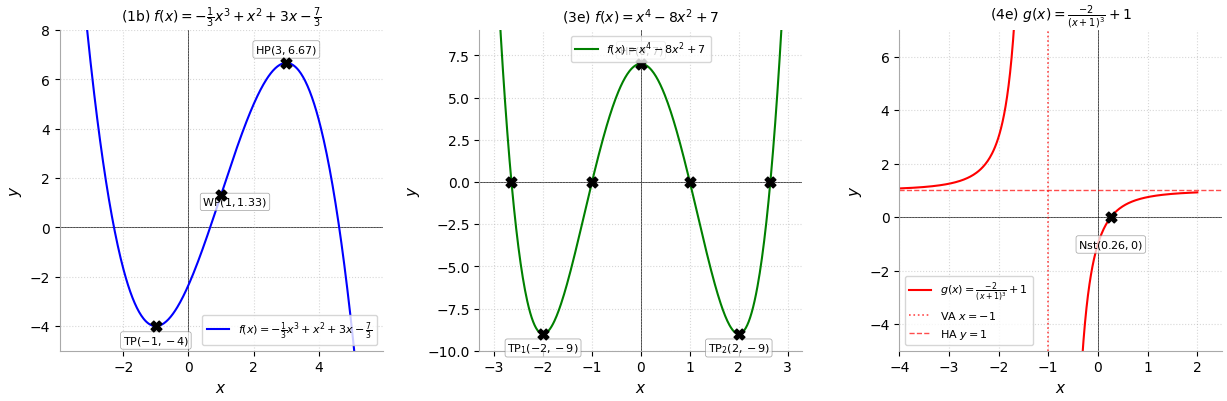
\includegraphics[width=0.8\textwidth]{grafiken/uebergreifend_alle_graphen.png.png}
    \captionof{figure}{Graphen der untersuchten Funktionen: (1b) $f(x) = -\frac{1}{3}x^3 + x^2 + 3x - \frac{7}{3}$, (3e) $f(x) = x^4 - 8x^2 + 7$, und (4e) $g(x) = \frac{-2}{(x+1)^3} + 1$.}
    \label{fig:uebergreifend_alle_graphen}
\end{center}

\end{loesungsumgebung}




\begin{aufgabenumgebung}{Produktregel trainieren}
Leite die folgenden Funktionen mit der Produktregel ab und vereinfache die Ergebnisse so weit wie möglich. Kontrolliere deine Ergebnisse für die ersten beiden Aufgaben, indem du die Terme zuerst ausmultiplizierst und dann ableitest.
\begin{enumerate}
    \item $f(x) = (x+2)(3x-4)$
    \item $g(x) = x^2(x^3+5x)$
    \item $h(t) = (t^2-1)(t^2+1)$ (Erkennst du hier eine binomische Formel, die das Ausmultiplizieren erleichtert?)
    \item $k(x) = (2x^3-x)(x^2+x+1)$
    \item $m(a) = (a^2+1)(a-1)$ (Leite nach $a$ ab.)
\end{enumerate}
\end{aufgabenumgebung}

\begin{loesungsumgebung}[loes:produktregel-trainieren]{Produktregel trainieren}
Wir verwenden die Produktregel $f'(x) = u'(x)v(x) + u(x)v'(x)$, um die Ableitungen zu bestimmen.

\begin{enumerate}[label=(\alph*)]
    \item \textbf{Funktion $f(x) = (x+2)(3x-4)$}
    \begin{itemize}
        \item \textbf{Mit Produktregel:} \\
        Sei $u(x) = x+2 \Rightarrow u'(x) = 1$. \\
        Sei $v(x) = 3x-4 \Rightarrow v'(x) = 3$.
        \begin{align*}
        f'(x) &= u'(x)v(x) + u(x)v'(x) \\
              &= 1 \cdot (3x-4) + (x+2) \cdot 3 \\
              &= 3x - 4 + 3x + 6 \\
              &= \mathbf{6x + 2}
        \end{align*}
        \item \textbf{Kontrolle durch Ausmultiplizieren:}
        $f(x) = (x+2)(3x-4) = 3x^2 - 4x + 6x - 8 = 3x^2 + 2x - 8$.
        $f'(x) = \frac{d}{dx}(3x^2 + 2x - 8) = 6x + 2$.
        Die Ergebnisse stimmen überein.
    \end{itemize}

    \item \textbf{Funktion $g(x) = x^2(x^3+5x)$}
    \begin{itemize}
        \item \textbf{Mit Produktregel:} \\
        Sei $u(x) = x^2 \Rightarrow u'(x) = 2x$. \\
        Sei $v(x) = x^3+5x \Rightarrow v'(x) = 3x^2+5$.
        \begin{align*}
        g'(x) &= u'(x)v(x) + u(x)v'(x) \\
              &= 2x(x^3+5x) + x^2(3x^2+5) \\
              &= 2x^4 + 10x^2 + 3x^4 + 5x^2 \\
              &= \mathbf{5x^4 + 15x^2}
        \end{align*}
        \item \textbf{Kontrolle durch Ausmultiplizieren:}
        $g(x) = x^2(x^3+5x) = x^5 + 5x^3$.
        $g'(x) = \frac{d}{dx}(x^5 + 5x^3) = 5x^4 + 15x^2$.
        Die Ergebnisse stimmen überein.
    \end{itemize}

    \item \textbf{Funktion $h(t) = (t^2-1)(t^2+1)$} \\
    \textit{Tipp:} Dies ist die 3. binomische Formel: $(A-B)(A+B) = A^2-B^2$.
    $h(t) = (t^2)^2 - 1^2 = t^4 - 1$.
    Ableiten der vereinfachten Form:
    $h'(t) = \frac{d}{dt}(t^4 - 1) = \mathbf{4t^3}$.
    \textit{Zur Übung auch mit Produktregel:} \\
    Sei $u(t) = t^2-1 \Rightarrow u'(t) = 2t$. \\
    Sei $v(t) = t^2+1 \Rightarrow v'(t) = 2t$.
    \begin{align*}
    h'(t) &= u'(t)v(t) + u(t)v'(t) \\
          &= 2t(t^2+1) + (t^2-1)(2t) \\
          &= 2t^3 + 2t + 2t^3 - 2t \\
          &= 4t^3
    \end{align*}
    Die Ergebnisse stimmen überein. Das Ausmultiplizieren war hier schneller.

    \item \textbf{Funktion $k(x) = (2x^3-x)(x^2+x+1)$}
    \begin{itemize}
        \item \textbf{Mit Produktregel:} \\
        Sei $u(x) = 2x^3-x \Rightarrow u'(x) = 6x^2-1$. \\
        Sei $v(x) = x^2+x+1 \Rightarrow v'(x) = 2x+1$.
        \begin{align*}
        k'(x) &= u'(x)v(x) + u(x)v'(x) \\
              &= (6x^2-1)(x^2+x+1) + (2x^3-x)(2x+1) \\
              &= (6x^4 + 6x^3 + 6x^2 - x^2 - x - 1) + (4x^4 + 2x^3 - 2x^2 - x) \\
              &= (6x^4 + 6x^3 + 5x^2 - x - 1) + (4x^4 + 2x^3 - 2x^2 - x) \\
              &= \mathbf{10x^4 + 8x^3 + 3x^2 - 2x - 1}
        \end{align*}
    \end{itemize}

    \item \textbf{Funktion $m(a) = (a^2+1)(a-1)$ (Ableitung nach $a$)}
    \begin{itemize}
        \item \textbf{Mit Produktregel:} \\
        Sei $u(a) = a^2+1 \Rightarrow u'(a) = 2a$. \\
        Sei $v(a) = a-1 \Rightarrow v'(a) = 1$.
        \begin{align*}
        m'(a) &= u'(a)v(a) + u(a)v'(a) \\
               &= 2a(a-1) + (a^2+1)(1) \\
               &= 2a^2 - 2a + a^2 + 1 \\
               &= \mathbf{3a^2 - 2a + 1}
        \end{align*}
        \textit{Kontrolle durch Ausmultiplizieren:}
        $m(a) = a^3 - a^2 + a - 1$.
        $m'(a) = 3a^2 - 2a + 1$. (Stimmt überein)
    \end{itemize}
\end{enumerate}

\end{loesungsumgebung}

\begin{aufgabenumgebung}[A:ProduktregelAnwendung]{Anwendung der Produktregel in einer Kurvendiskussion (vereinfacht)}
Gegeben sei die Funktion $f(x) = x \cdot (x-3)^2$.
\begin{enumerate}
    \item \textbf{Definitionsbereich und Verhalten im Unendlichen:} Bestimme $D_f$ und untersuche $\lim_{x \to \pm\infty} f(x)$.
    \item \textbf{Nullstellen:} Bestimme die Nullstellen von $f(x)$ direkt aus der faktorisierten Form. Welche Vielfachheit haben sie? Was bedeutet das für den Graphen?
    \item \textbf{Erste Ableitung mit Produktregel:}
        Identifiziere $u(x)=x$ und $v(x)=(x-3)^2$. 
        Bilde $f'(x)$ mit der Produktregel. Vereinfache $f'(x)$ so weit wie möglich (Tipp: $(x-3)$ ausklammern).
    \item \textbf{Extremstellen:} Bestimme die Nullstellen von $f'(x)$. Untersuche das Vorzeichen von $f'(x)$ (Monotonieintervalle), um die Art der Extremstellen zu bestimmen. Berechne die y-Koordinaten der Extrempunkte.
    \item \textbf{Skizze:} Skizziere den Graphen von $f(x)$ unter Verwendung deiner Ergebnisse.
\end{enumerate}
Diese Aufgabe zeigt, wie die Produktregel auch bei der Analyse von Polynomfunktionen nützlich sein kann, besonders wenn sie in faktorisierter Form vorliegen oder entstehen.
\end{aufgabenumgebung}

\begin{loesungsumgebung}[loes:A:ProduktregelAnwendung]{Anwendung der Produktregel in einer Kurvendiskussion}
Wir untersuchen die Funktion $f(x) = x \cdot (x-3)^2$.

\begin{enumerate}[label=(\alph*)]
    \item \textbf{Definitionsbereich und Verhalten im Unendlichen:}
    \begin{itemize}
        \item \textbf{Definitionsbereich ($D_f$):} Da $f(x)$ eine Polynomfunktion ist (nach Ausmultiplizieren $f(x) = x(x^2-6x+9) = x^3-6x^2+9x$), ist der Definitionsbereich $\mathbf{D_f = \mathbb{R}}$.
        \item \textbf{Verhalten im Unendlichen ($\lim_{x \to \pm\infty} f(x)$):}
        Der Leitterm der ausmultiplizierten Form $x^3-6x^2+9x$ ist $x^3$.
        Für $x \to \infty$: $\lim_{x \to \infty} f(x) = \lim_{x \to \infty} x^3 = \mathbf{+\infty}$.
        Für $x \to -\infty$: $\lim_{x \to -\infty} f(x) = \lim_{x \to -\infty} x^3 = \mathbf{-\infty}$.
        (Der Graph verläuft von links unten nach rechts oben).
    \end{itemize}

    \item \textbf{Nullstellen:}
    Wir setzen $f(x)=0$: $x \cdot (x-3)^2 = 0$.
    Nach dem Satz vom Nullprodukt gilt:
    \begin{itemize}
        \item $x_1 = 0$. Dies ist eine \textbf{einfache Nullstelle} (der Faktor $x$ hat den Exponenten 1). Der Graph schneidet hier die x-Achse.
        \item $(x-3)^2 = 0 \Rightarrow x-3=0 \Rightarrow x_2 = 3$. Dies ist eine \textbf{doppelte Nullstelle} (der Faktor $(x-3)$ hat den Exponenten 2). Der Graph berührt hier die x-Achse.
    \end{itemize}
    Die Nullstellen sind $N_1(0|0)$ und $N_2(3|0)$.

    \item \textbf{Erste Ableitung mit Produktregel:}
    Sei $u(x)=x$ und $v(x)=(x-3)^2$.
    Dann ist $u'(x)=1$.
    Für $v'(x)$ verwenden wir den Tipp oder leiten ausmultipliziert ab: $v(x) = x^2-6x+9 \Rightarrow v'(x) = 2x-6 = 2(x-3)$.
    Nach der Produktregel $f'(x) = u'(x)v(x) + u(x)v'(x)$:
    \begin{align*}
    f'(x) &= 1 \cdot (x-3)^2 + x \cdot [2(x-3)] \\
          &= (x-3)^2 + 2x(x-3)
    \end{align*}
    Wir klammern $(x-3)$ aus:
    \begin{align*}
    f'(x) &= (x-3) \cdot [(x-3) + 2x] \\
          &= (x-3) \cdot (3x-3) \\
          &= \mathbf{3(x-3)(x-1)}
    \end{align*}

    \item \textbf{Extremstellen:}
    Notwendige Bedingung: $f'(x_E)=0$.
    $3(x-3)(x-1) = 0$.
    Die Kandidaten für Extremstellen sind $x_{E1} = 1$ und $x_{E2} = 3$.
    Untersuchung des Vorzeichens von $f'(x) = 3(x-1)(x-3)$:
    Der Graph von $f'(x)$ ist eine nach oben geöffnete Parabel mit Nullstellen bei $1$ und $3$.
    \begin{itemize}
        \item Für $x < 1$ (z.B. $x=0$): $f'(0) = 3(-1)(-3) = 9 > 0 \implies f(x)$ ist streng monoton steigend.
        \item Für $1 < x < 3$ (z.B. $x=2$): $f'(2) = 3(1)(-1) = -3 < 0 \implies f(x)$ ist streng monoton fallend.
        \item Für $x > 3$ (z.B. $x=4$): $f'(4) = 3(3)(1) = 9 > 0 \implies f(x)$ ist streng monoton steigend.
    \end{itemize}
    Art und Koordinaten der Extrempunkte:
    \begin{itemize}
        \item Bei $x_{E1} = 1$: Vorzeichenwechsel von $f'(x)$ von $+$ nach $- \Rightarrow$ Lokaler Hochpunkt.
        $y_{E1} = f(1) = 1 \cdot (1-3)^2 = 1 \cdot (-2)^2 = 4$.
        $\rightarrow \mathbf{HP(1|4)}$.
        \item Bei $x_{E2} = 3$: Vorzeichenwechsel von $f'(x)$ von $-$ nach $+ \Rightarrow$ Lokaler Tiefpunkt.
        $y_{E2} = f(3) = 3 \cdot (3-3)^2 = 3 \cdot 0^2 = 0$.
        $\rightarrow \mathbf{TP(3|0)}$. (Dies ist auch die doppelte Nullstelle, was konsistent ist).
    \end{itemize}

    \item \textbf{Skizze:}
    Der Graph der Funktion $f(x) = x(x-3)^2$ ist ein Polynom 3. Grades.
    \begin{itemize}
        \item Er verläuft von links unten ($x \to -\infty, f(x) \to -\infty$) nach rechts oben ($x \to \infty, f(x) \to \infty$).
        \item Er schneidet die x-Achse bei $x=0$ (einfache Nullstelle) und berührt die x-Achse bei $x=3$ (doppelte Nullstelle, gleichzeitig Tiefpunkt).
        \item Er hat einen lokalen Hochpunkt bei $HP(1|4)$.
        \item Der y-Achsenabschnitt ist $(0|0)$.
    \end{itemize}
    \begin{center}
    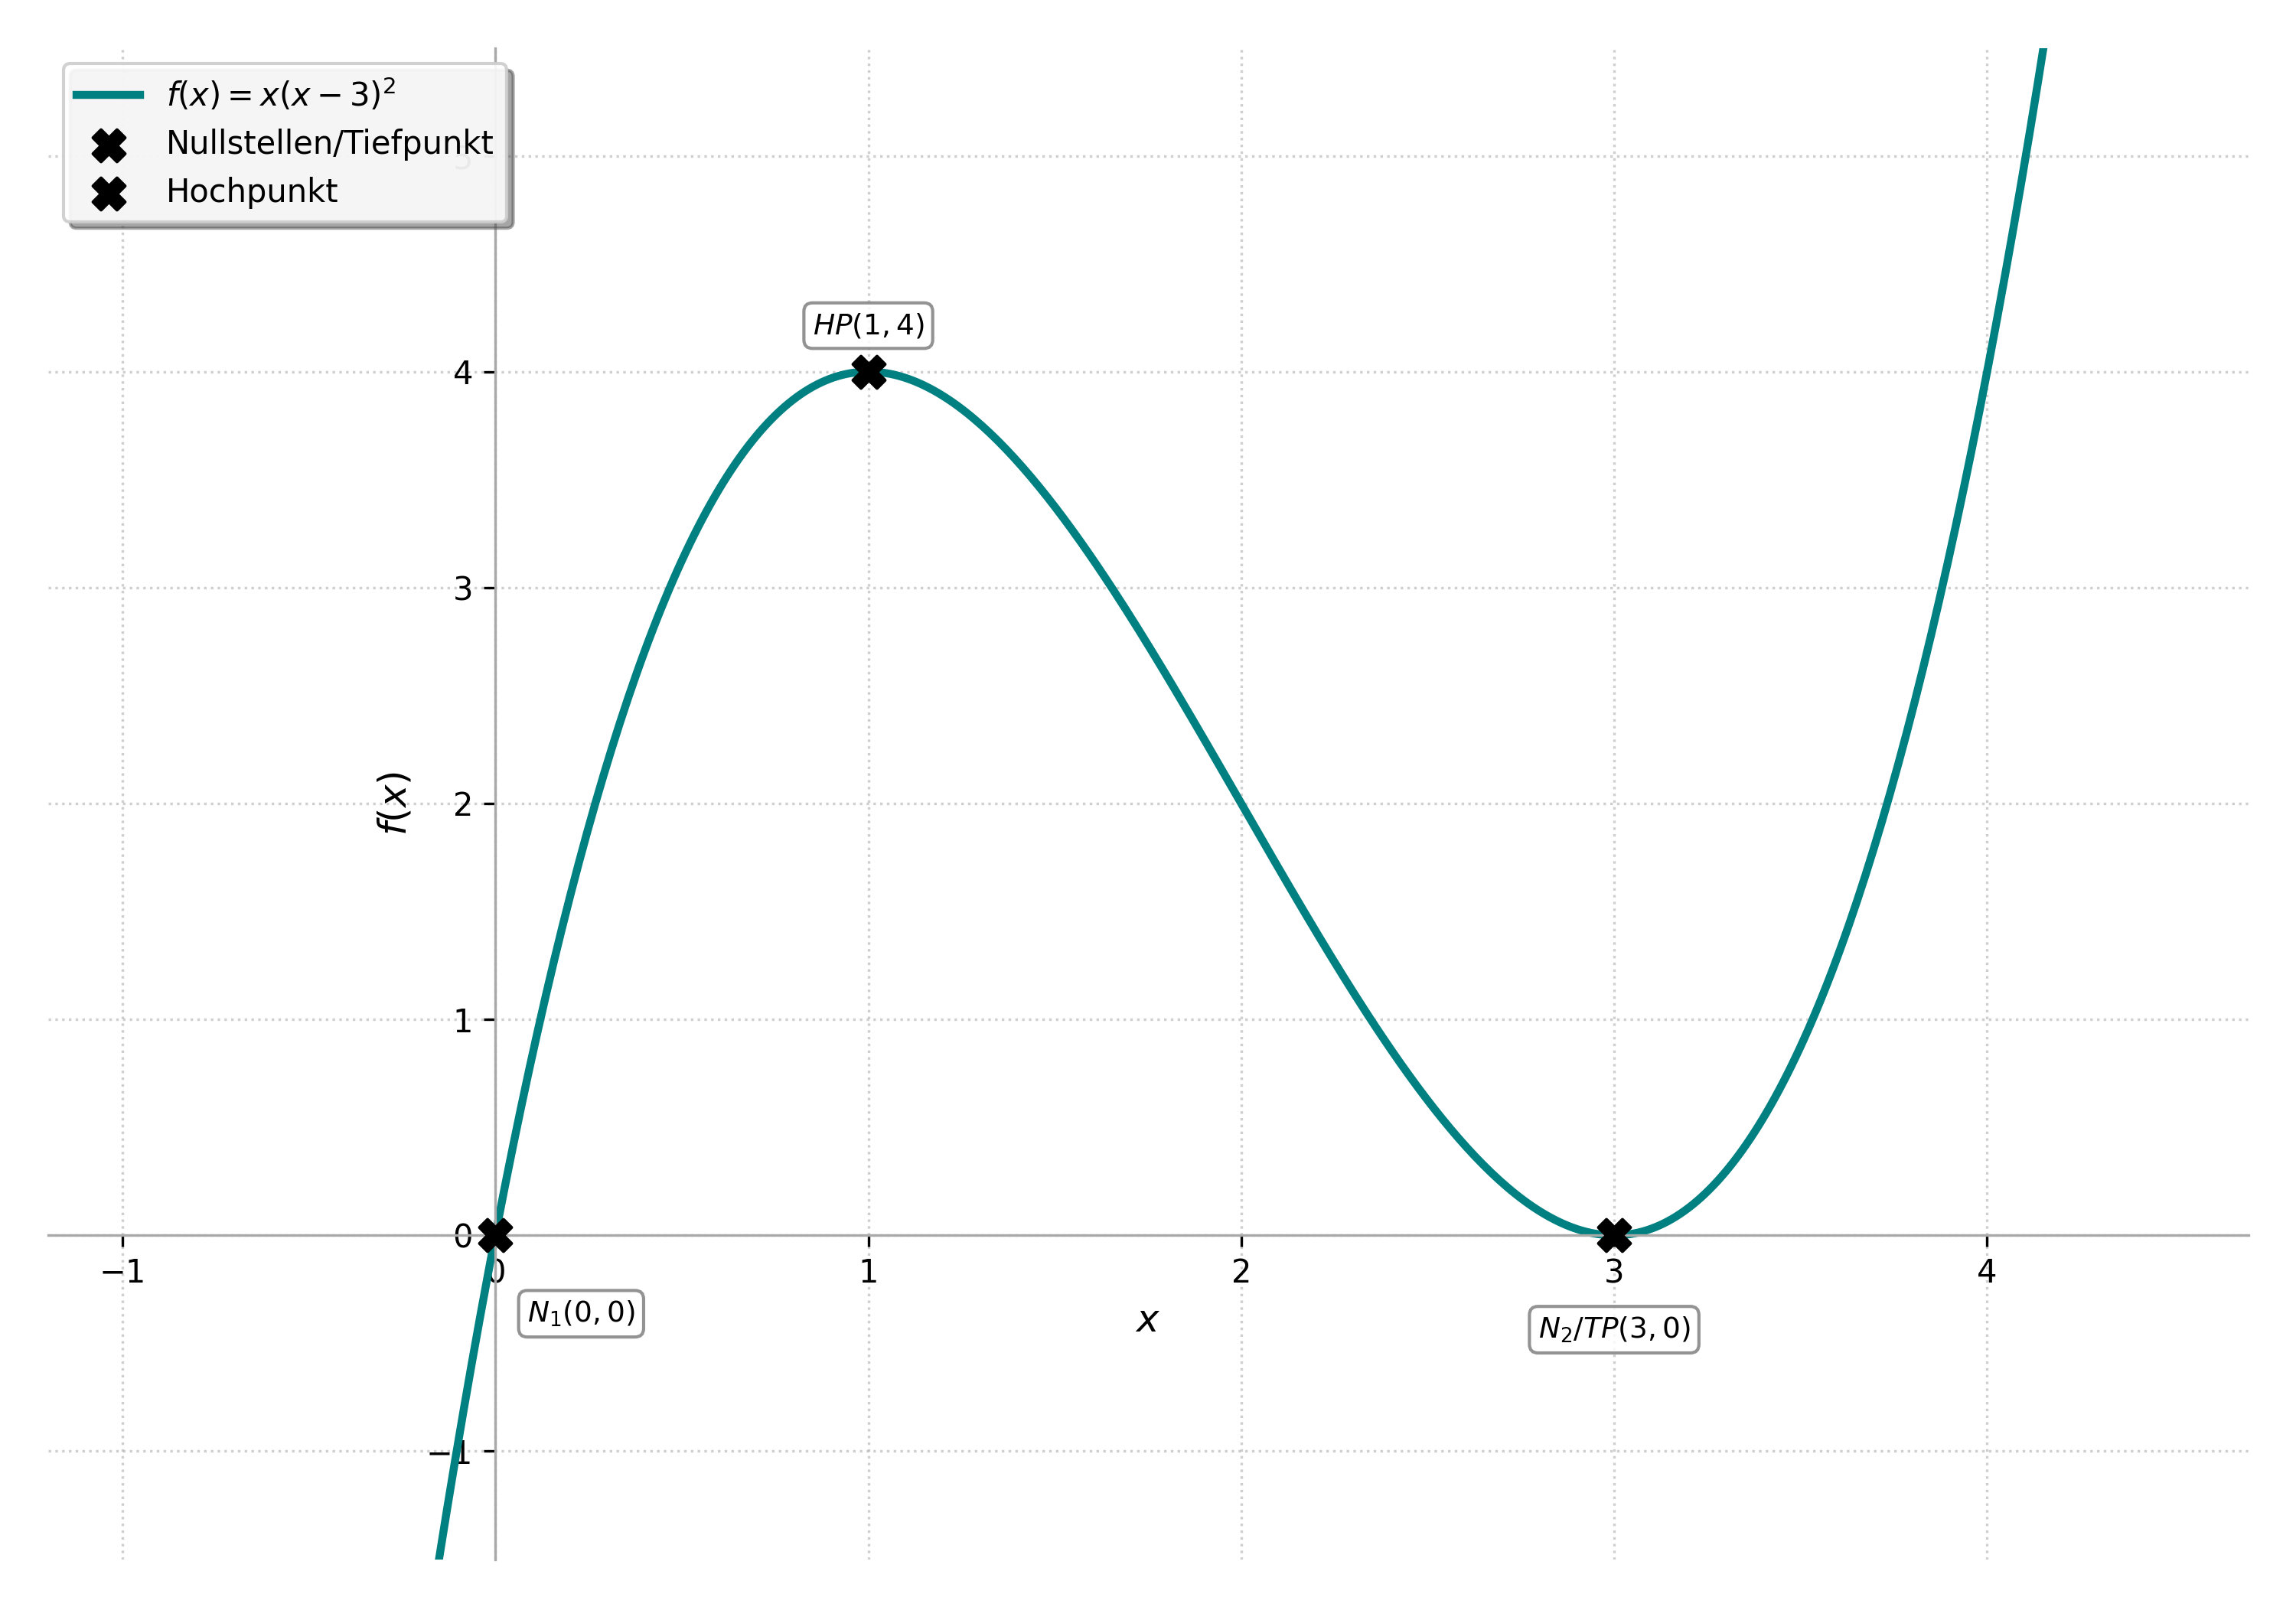
\includegraphics[width=0.8\textwidth]{grafiken/f_produktregel_anwendung_graph.png}
    % --- Beschreibung der Skizze ---
    % Die Skizze zeigt den Graphen eines Polynoms 3. Grades.
    % Nullstellen: (0|0) - Schnittpunkt; (3|0) - Berührpunkt (Tiefpunkt).
    % Lokaler Hochpunkt: (1|4).
    % Verlauf: Kommt von links unten, steigt zum HP(1|4), fällt zum TP(3|0) (berührt x-Achse), steigt dann nach rechts oben.
    \captionof{figure}{Graph der Funktion $f(x) = x(x-3)^2$.}
    \label{fig:f_produktregel_anwendung_graph}
    \end{center}
\end{enumerate}

\end{loesungsumgebung}


\begin{aufgabenumgebung}{Quotientenregel trainieren}
Leite die folgenden Funktionen mit der Quotientenregel ab und vereinfache die Zähler der Ergebnisse so weit wie möglich. Gib auch den Definitionsbereich der ursprünglichen Funktion an.
\begin{enumerate}
    \item $f(x) = \frac{x}{x+1}$
    \item $g(x) = \frac{3x-2}{x^2}$ (Tipp: Dies könnte man auch als $g(x) = (3x-2)x^{-2}$ mit der Produktregel oder nach Aufteilen des Bruchs $\frac{3x}{x^2} - \frac{2}{x^2} = \frac{3}{x} - \frac{2}{x^2}$ mit Potenz-/Faktorregeln ableiten. Vergleiche die Ergebnisse!)
    \item $h(t) = \frac{t^2+2t}{t-1}$
    \item $k(x) = \frac{5}{2x+3}$ (Hier ist $u(x)=5$, also $u'(x)=0$. Was bedeutet das für die Formel?)
\end{enumerate}
\end{aufgabenumgebung}



\begin{loesungsumgebung}[loes:quotientenregel-trainieren]{Quotientenregel trainieren}
Wir verwenden die Quotientenregel $f'(x) = \frac{u'(x)v(x) - u(x)v'(x)}{[v(x)]^2}$, um die Ableitungen zu bestimmen.

\begin{enumerate}[label=(\alph*)]
    \item \textbf{Funktion $f(x) = \frac{x}{x+1}$}
    \begin{itemize}
        \item \textbf{Definitionsbereich:} Der Nenner darf nicht Null sein: $x+1 \neq 0 \Rightarrow x \neq -1$. $D_f = \mathbb{R} \setminus \{-1\}$.
        \item \textbf{Ableitung mit Quotientenregel:} \\
        Sei $u(x) = x \Rightarrow u'(x) = 1$. \\
        Sei $v(x) = x+1 \Rightarrow v'(x) = 1$.
        \begin{align*}
        f'(x) &= \frac{u'(x)v(x) - u(x)v'(x)}{[v(x)]^2} \\
              &= \frac{1 \cdot (x+1) - x \cdot 1}{(x+1)^2} \\
              &= \frac{x+1-x}{(x+1)^2} \\
              &= \mathbf{\frac{1}{(x+1)^2}}
        \end{align*}
    \end{itemize}

    \item \textbf{Funktion $g(x) = \frac{3x-2}{x^2}$}
    \begin{itemize}
        \item \textbf{Definitionsbereich:} $x^2 \neq 0 \Rightarrow x \neq 0$. $D_g = \mathbb{R} \setminus \{0\}$.
        \item \textbf{Ableitung mit Quotientenregel:} \\
        Sei $u(x) = 3x-2 \Rightarrow u'(x) = 3$. \\
        Sei $v(x) = x^2 \Rightarrow v'(x) = 2x$.
        \begin{align*}
        g'(x) &= \frac{3 \cdot x^2 - (3x-2) \cdot 2x}{(x^2)^2} \\
              &= \frac{3x^2 - (6x^2 - 4x)}{x^4} \\
              &= \frac{3x^2 - 6x^2 + 4x}{x^4} \\
              &= \frac{-3x^2 + 4x}{x^4} \\
              &= \frac{x(-3x + 4)}{x \cdot x^3} \quad (\text{für } x \neq 0) \\
              &= \mathbf{\frac{-3x + 4}{x^3}} \quad \text{oder } \mathbf{-\frac{3}{x^2} + \frac{4}{x^3}}
        \end{align*}
        \item \textbf{Vergleich mit alternativen Methoden (Tipp):}
        \begin{itemize}
            \item \textit{Als Produkt $g(x) = (3x-2)x^{-2}$:} \\
            $u(x)=3x-2 \Rightarrow u'(x)=3$. $w(x)=x^{-2} \Rightarrow w'(x)=-2x^{-3}$.
            $g'(x) = 3x^{-2} + (3x-2)(-2x^{-3}) = \frac{3}{x^2} - \frac{6x}{x^3} + \frac{4}{x^3} = \frac{3}{x^2} - \frac{6}{x^2} + \frac{4}{x^3} = -\frac{3}{x^2} + \frac{4}{x^3} = \frac{-3x+4}{x^3}$. (Stimmt überein)
            \item \textit{Nach Aufteilen des Bruchs $g(x) = \frac{3x}{x^2} - \frac{2}{x^2} = 3x^{-1} - 2x^{-2}$:} \\
            $g'(x) = 3(-1)x^{-2} - 2(-2)x^{-3} = -3x^{-2} + 4x^{-3} = -\frac{3}{x^2} + \frac{4}{x^3} = \frac{-3x+4}{x^3}$. (Stimmt überein)
        \end{itemize}
    \end{itemize}

    \item \textbf{Funktion $h(t) = \frac{t^2+2t}{t-1}$}
    \begin{itemize}
        \item \textbf{Definitionsbereich:} $t-1 \neq 0 \Rightarrow t \neq 1$. $D_h = \mathbb{R} \setminus \{1\}$.
        \item \textbf{Ableitung mit Quotientenregel:} \\
        Sei $u(t) = t^2+2t \Rightarrow u'(t) = 2t+2$. \\
        Sei $v(t) = t-1 \Rightarrow v'(t) = 1$.
        \begin{align*}
        h'(t) &= \frac{(2t+2)(t-1) - (t^2+2t)(1)}{(t-1)^2} \\
              &= \frac{(2t^2 - 2t + 2t - 2) - (t^2+2t)}{(t-1)^2} \\
              &= \frac{2t^2 - 2 - t^2 - 2t}{(t-1)^2} \\
              &= \mathbf{\frac{t^2 - 2t - 2}{(t-1)^2}}
        \end{align*}
    \end{itemize}

    \item \textbf{Funktion $k(x) = \frac{5}{2x+3}$}
    \begin{itemize}
        \item \textbf{Definitionsbereich:} $2x+3 \neq 0 \Rightarrow 2x \neq -3 \Rightarrow x \neq -\frac{3}{2}$. $D_k = \mathbb{R} \setminus \{-\frac{3}{2}\}$.
        \item \textbf{Ableitung mit Quotientenregel:} \\
        Sei $u(x) = 5 \Rightarrow u'(x) = 0$. \\
        Sei $v(x) = 2x+3 \Rightarrow v'(x) = 2$.
        \begin{align*}
        k'(x) &= \frac{0 \cdot (2x+3) - 5 \cdot 2}{(2x+3)^2} \\
              &= \frac{0 - 10}{(2x+3)^2} \\
              &= \mathbf{\frac{-10}{(2x+3)^2}}
        \end{align*}
        \textit{Anmerkung:} Da $u(x)$ eine Konstante ist, wird der erste Term im Zähler der Quotientenregel ($u'v$) Null. Die Formel vereinfacht sich zu $k'(x) = \frac{-uv'}{v^2}$. Dies entspricht auch der Ableitung mittels Kettenregel für $k(x) = 5(2x+3)^{-1}$: $k'(x) = 5 \cdot (-1)(2x+3)^{-2} \cdot 2 = -10(2x+3)^{-2}$.
    \end{itemize}
\end{enumerate}

\end{loesungsumgebung}



\begin{aufgabenumgebung}{Anwendung der neuen Regeln in Kontexten}
\begin{enumerate}
    \item \textbf{Umsatzfunktion:} Ein Unternehmen verkauft ein Produkt. Die Preis-Absatz-Funktion (Nachfragefunktion) sei $p(x) = 100 - 0.5x$, wobei $x$ die verkaufte Menge und $p(x)$ der Preis pro Stück ist. Der Umsatz $U(x)$ ist Preis mal Menge, also $U(x) = p(x) \cdot x = (100-0.5x)x$.
        \begin{itemize}
            \item Bestimme die Umsatzfunktion $U(x)$.
            \item Bilde die erste Ableitung $U'(x)$ (Grenzerlös). Du kannst dies tun, indem du $U(x)$ zuerst ausmultiplizierst oder indem du die Produktregel auf $p(x) \cdot x$ anwendest. Vergleiche beide Wege.
            \item Bei welcher Verkaufsmenge $x$ wird der Grenzerlös Null? Was könnte das für den Gesamtumsatz bedeuten?
        \end{itemize}
    \item \textbf{Durchschnittskosten:} Die Kostenfunktion eines Unternehmens sei $K(x) = 0.1x^3 - 2x^2 + 50x + 100$. Die Durchschnittskosten (Stückkosten) sind $k(x) = \frac{K(x)}{x}$.
        \begin{itemize}
            \item Schreibe die Funktion für die Durchschnittskosten $k(x)$ auf.
            \item Bilde die erste Ableitung $k'(x)$ mit der Quotientenregel.
            \item (Für Experten): Versuche, die Stelle zu finden, an der die Durchschnittskosten minimal sind (also $k'(x)=0$ setzen und nach $x$ auflösen – das kann hier schwierig werden, aber der Ansatz ist wichtig).
        \end{itemize}
\end{enumerate}
\end{aufgabenumgebung}



\begin{loesungsumgebung}[loes:anwendung-produkt-quotientenregel-kontext]{Anwendung der neuen Regeln in Kontexten}

\begin{enumerate}[label=(\alph*)]
    \item \textbf{Umsatzfunktion:}
    Gegeben ist die Preis-Absatz-Funktion $p(x) = 100 - 0.5x$. Der Umsatz ist $U(x) = p(x) \cdot x$.
    \begin{itemize}
        \item \textbf{Bestimme die Umsatzfunktion $U(x)$:}
        $U(x) = (100 - 0.5x) \cdot x = \mathbf{100x - 0.5x^2}$.

        \item \textbf{Bilde die erste Ableitung $U'(x)$ (Grenzerlös):}
        \textit{Weg 1: Ableiten der ausmultiplizierten Form}
        $U(x) = 100x - 0.5x^2$.
        $U'(x) = \frac{d}{dx}(100x - 0.5x^2) = 100 - 0.5 \cdot 2x = \mathbf{100 - x}$.

        \textit{Weg 2: Anwendung der Produktregel auf $U(x) = (100-0.5x)x$}
        Sei $u(x) = 100-0.5x \Rightarrow u'(x) = -0.5$.
        Sei $v(x) = x \Rightarrow v'(x) = 1$.
        $U'(x) = u'(x)v(x) + u(x)v'(x) = (-0.5)(x) + (100-0.5x)(1)$
        $U'(x) = -0.5x + 100 - 0.5x = \mathbf{100 - x}$.
        \textit{Vergleich:} Beide Wege führen zum selben Ergebnis.

        \item \textbf{Bei welcher Verkaufsmenge $x$ wird der Grenzerlös Null? Was könnte das für den Gesamtumsatz bedeuten?}
        Setze $U'(x) = 0$:
        $100 - x = 0 \Rightarrow x = 100$.
        Der Grenzerlös wird bei einer Verkaufsmenge von $\mathbf{x=100}$ Null.
        \textit{Bedeutung:} Wenn der Grenzerlös Null ist, bedeutet das, dass eine weitere verkaufte Einheit keinen zusätzlichen Umsatz mehr generiert (oder der zusätzliche Umsatz ist vernachlässigbar klein). Da die Umsatzfunktion $U(x) = -0.5x^2 + 100x$ eine nach unten geöffnete Parabel ist ($a=-0.5 < 0$), befindet sich an der Stelle, an der die erste Ableitung Null ist, das \textbf{Maximum des Gesamtumsatzes}. Bei einer Verkaufsmenge von 100 Stück ist der Umsatz also maximal.
    \end{itemize}

    \item \textbf{Durchschnittskosten:}
    Kostenfunktion $K(x) = 0.1x^3 - 2x^2 + 50x + 100$. Durchschnittskosten $k(x) = \frac{K(x)}{x}$.
    \begin{itemize}
        \item \textbf{Schreibe die Funktion für die Durchschnittskosten $k(x)$ auf:}
        $k(x) = \frac{0.1x^3 - 2x^2 + 50x + 100}{x}$.
        Für den Definitionsbereich $x>0$ (da $x$ eine Menge ist) können wir auch schreiben:
        $k(x) = 0.1x^2 - 2x + 50 + \frac{100}{x}$.

        \item \textbf{Bilde die erste Ableitung $k'(x)$ mit der Quotientenregel:}
        Für $k(x) = \frac{K(x)}{x}$:
        Sei $u(x) = K(x) = 0.1x^3 - 2x^2 + 50x + 100 \Rightarrow u'(x) = K'(x) = 0.3x^2 - 4x + 50$.
        Sei $v(x) = x \Rightarrow v'(x) = 1$.
        \begin{align*}
        k'(x) &= \frac{u'(x)v(x) - u(x)v'(x)}{[v(x)]^2} \\
              &= \frac{(0.3x^2 - 4x + 50) \cdot x - (0.1x^3 - 2x^2 + 50x + 100) \cdot 1}{x^2} \\
              &= \frac{0.3x^3 - 4x^2 + 50x - 0.1x^3 + 2x^2 - 50x - 100}{x^2} \\
              &= \frac{0.2x^3 - 2x^2 - 100}{x^2} \\
              &= \mathbf{0.2x - 2 - \frac{100}{x^2}} \quad (\text{für } x \neq 0)
        \end{align*}
        \textit{Kontrolle mit $k(x) = 0.1x^2 - 2x + 50 + 100x^{-1}$:}
        $k'(x) = 0.2x - 2 - 100x^{-2} = 0.2x - 2 - \frac{100}{x^2}$. (Stimmt überein).

        \item \textbf{(Für Experten): Stelle finden, an der die Durchschnittskosten minimal sind ($k'(x)=0$):}
        Wir setzen $k'(x) = 0$:
        $0.2x - 2 - \frac{100}{x^2} = 0$.
        Multiplikation mit $x^2$ (für $x \neq 0$):
        $0.2x^3 - 2x^2 - 100 = 0$.
        Multiplikation mit 5, um ganzzahlige Koeffizienten zu erhalten (optional):
        $x^3 - 10x^2 - 500 = 0$.
        Dies ist eine kubische Gleichung. Ihre exakte algebraische Lösung ist nicht trivial und erfordert typischerweise das Raten einer Nullstelle (Teiler von 500) oder numerische Verfahren.
        Wenn $P(x) = x^3 - 10x^2 - 500$:
        $P(10) = 1000 - 1000 - 500 = -500$.
        $P(11) = 1331 - 1210 - 500 = -379$.
        $P(12) = 1728 - 1440 - 500 = -212$.
        $P(13) = 2197 - 1690 - 500 = 7$.
        Da $P(12) < 0$ und $P(13) > 0$, liegt eine Nullstelle (und somit eine potenzielle Stelle minimaler Durchschnittskosten) zwischen $x=12$ und $x=13$. Die exakte Stelle müsste numerisch oder mit fortgeschritteneren Methoden zur Lösung kubischer Gleichungen bestimmt werden. Der Ansatz, $k'(x)=0$ zu setzen, ist der korrekte Weg, um das Minimum der Durchschnittskosten zu finden. (Dieser Punkt ist auch bekannt als das Betriebsoptimum, wo die Grenzkosten $K'(x)$ die Durchschnittskosten $k(x)$ schneiden).
    \end{itemize}
\end{enumerate}

\end{loesungsumgebung}

\begin{aufgabenumgebung}{Kettenregel trainieren}
Leite die folgenden Funktionen mit der Kettenregel ab. Identifiziere zuerst sorgfältig die äußere und die innere Funktion.
\begin{enumerate}
    \item $f(x) = (x^2+1)^4$
    \item $g(x) = (5-3x)^7$
    \item $h(t) = \sqrt{t^2+3t}$ (Tipp: $\sqrt{u} = u^{1/2}$)
    \item $k(x) = \frac{1}{(x^3-2x)^2}$ (Tipp: $k(x) = (x^3-2x)^{-2}$)
    \item $m(x) = (ax^2+b)^n$ (wobei $a,b,n$ Konstanten sind. Was ist die Ableitung?)
\end{enumerate}
\end{aufgabenumgebung}

\begin{loesungsumgebung}[loes:kettenregel-trainieren]{Kettenregel trainieren}
Wir identifizieren jeweils die äußere Funktion $a(u)$ und die innere Funktion $u=i(x)$, bilden deren Ableitungen $a'(u)$ und $i'(x)$ und wenden dann die Kettenregel $f'(x) = a'(i(x)) \cdot i'(x)$ an.

\begin{enumerate}[label=(\alph*)]
    \item \textbf{Funktion $f(x) = (x^2+1)^4$}
    \begin{itemize}
        \item Äußere Funktion: $a(u) = u^4 \Rightarrow a'(u) = 4u^3$.
        \item Innere Funktion: $i(x) = x^2+1 \Rightarrow i'(x) = 2x$.
    \end{itemize}
    Anwendung der Kettenregel:
    \begin{align*}
    f'(x) &= a'(i(x)) \cdot i'(x) \\
          &= 4(x^2+1)^3 \cdot (2x) \\
          &= \mathbf{8x(x^2+1)^3}
    \end{align*}

    \item \textbf{Funktion $g(x) = (5-3x)^7$}
    \begin{itemize}
        \item Äußere Funktion: $a(u) = u^7 \Rightarrow a'(u) = 7u^6$.
        \item Innere Funktion: $i(x) = 5-3x \Rightarrow i'(x) = -3$.
    \end{itemize}
    Anwendung der Kettenregel:
    \begin{align*}
    g'(x) &= a'(i(x)) \cdot i'(x) \\
          &= 7(5-3x)^6 \cdot (-3) \\
          &= \mathbf{-21(5-3x)^6}
    \end{align*}

    \item \textbf{Funktion $h(t) = \sqrt{t^2+3t}$} \\
    Tipp: $\sqrt{u} = u^{1/2}$. Also $h(t) = (t^2+3t)^{1/2}$.
    \begin{itemize}
        \item Äußere Funktion: $a(u) = u^{1/2} \Rightarrow a'(u) = \frac{1}{2}u^{-1/2} = \frac{1}{2\sqrt{u}}$.
        \item Innere Funktion: $i(t) = t^2+3t \Rightarrow i'(t) = 2t+3$.
    \end{itemize}
    Anwendung der Kettenregel:
    \begin{align*}
    h'(t) &= a'(i(t)) \cdot i'(t) \\
          &= \frac{1}{2\sqrt{t^2+3t}} \cdot (2t+3) \\
          &= \mathbf{\frac{2t+3}{2\sqrt{t^2+3t}}}
    \end{align*}

    \item \textbf{Funktion $k(x) = \frac{1}{(x^3-2x)^2}$} \\
    Tipp: $k(x) = (x^3-2x)^{-2}$.
    \begin{itemize}
        \item Äußere Funktion: $a(u) = u^{-2} \Rightarrow a'(u) = -2u^{-3} = \frac{-2}{u^3}$.
        \item Innere Funktion: $i(x) = x^3-2x \Rightarrow i'(x) = 3x^2-2$.
    \end{itemize}
    Anwendung der Kettenregel:
    \begin{align*}
    k'(x) &= a'(i(x)) \cdot i'(x) \\
          &= \frac{-2}{(x^3-2x)^3} \cdot (3x^2-2) \\
          &= \mathbf{\frac{-2(3x^2-2)}{(x^3-2x)^3}} \quad \text{oder} \quad \mathbf{\frac{-6x^2+4}{(x^3-2x)^3}}
    \end{align*}

    \item \textbf{Funktion $m(x) = (ax^2+b)^n$} (wobei $a,b,n$ Konstanten sind)
    \begin{itemize}
        \item Äußere Funktion: $a_u(u) = u^n \Rightarrow a_u'(u) = nu^{n-1}$. (Der Index $u$ bei $a_u$ dient zur Unterscheidung vom Parameter $a$).
        \item Innere Funktion: $i(x) = ax^2+b \Rightarrow i'(x) = 2ax$ (da $b$ eine Konstante ist).
    \end{itemize}
    Anwendung der Kettenregel:
    \begin{align*}
    m'(x) &= a_u'(i(x)) \cdot i'(x) \\
           &= n(ax^2+b)^{n-1} \cdot (2ax) \\
           &= \mathbf{2anx(ax^2+b)^{n-1}}
    \end{align*}
    Dies ist die verallgemeinerte Potenzregel für eine innere lineare oder quadratische Funktion.
\end{enumerate}

\end{loesungsumgebung}



\begin{aufgabenumgebung}[A:KombinierteAnwendung]{Kombinierte Anwendung der Ableitungsregeln}
Leite die folgenden Funktionen ab. Gib an, welche Regeln du in welcher Reihenfolge anwendest.
\begin{enumerate}
    \item $f(x) = x^2 \cdot (2x+1)^3$ (Produkt- und Kettenregel)
    \item $g(x) = \frac{(x^2-1)^2}{x}$ (Quotienten- und Kettenregel, oder erst Zähler ausmultiplizieren)
    \item $h(t) = t \cdot \sqrt{1-t^2}$ (Produkt- und Kettenregel)
    \item \textbf{Für Tüftler:} Untersuche die Funktion $f(x) = x \cdot (x-4)^3$ auf Nullstellen, Monotonie und Extrempunkte. Skizziere den Graphen. (Diese Funktion ähnelt der Aufgabe \ref{A:ProduktregelAnwendung}, erfordert aber nun die Kettenregel für $v'(x)$.)
\end{enumerate}
\end{aufgabenumgebung}

\begin{loesungsumgebung}[loes:A:KombinierteAnwendung]{Kombinierte Anwendung der Ableitungsregeln}

\begin{enumerate}[label=(\alph*)]
    \item \textbf{Funktion $f(x) = x^2 \cdot (2x+1)^3$} \\
    Wir wenden die \textbf{Produktregel} an: $f'(x) = u'(x)v(x) + u(x)v'(x)$.
    Sei $u(x) = x^2 \Rightarrow u'(x) = 2x$.
    Sei $v(x) = (2x+1)^3$. Für $v'(x)$ benötigen wir die \textbf{Kettenregel}:
    Äußere Funktion $a_v(w) = w^3 \Rightarrow a_v'(w) = 3w^2$.
    Innere Funktion $i_v(x) = 2x+1 \Rightarrow i_v'(x) = 2$.
    Also $v'(x) = a_v'(i_v(x)) \cdot i_v'(x) = 3(2x+1)^2 \cdot 2 = 6(2x+1)^2$.
    \begin{align*}
    f'(x) &= (2x) \cdot (2x+1)^3 + (x^2) \cdot [6(2x+1)^2] \\
          &= (2x+1)^2 [2x(2x+1) + 6x^2] \quad (\text{Ausklammern von } (2x+1)^2) \\
          &= (2x+1)^2 [4x^2 + 2x + 6x^2] \\
          &= (2x+1)^2 (10x^2 + 2x) \\
          &= (2x+1)^2 \cdot 2x(5x+1) \\
          &= \mathbf{2x(5x+1)(2x+1)^2}
    \end{align*}
    \textit{Verwendete Regeln: Produktregel, Kettenregel, Potenzregel, Faktorregel, Summenregel.}

    \item \textbf{Funktion $g(x) = \frac{(x^2-1)^2}{x}$} \\
    \textit{Weg 1: Mit Quotienten- und Kettenregel.} $g(x) = \frac{u(x)}{v(x)}$.
    Sei $u(x) = (x^2-1)^2$. Für $u'(x)$ Kettenregel: $a_u(w)=w^2 \Rightarrow a_u'(w)=2w$; $i_u(x)=x^2-1 \Rightarrow i_u'(x)=2x$.
    Also $u'(x) = 2(x^2-1) \cdot 2x = 4x(x^2-1)$.
    Sei $v(x) = x \Rightarrow v'(x) = 1$.
    \begin{align*}
    g'(x) &= \frac{u'(x)v(x) - u(x)v'(x)}{[v(x)]^2} \\
          &= \frac{4x(x^2-1) \cdot x - (x^2-1)^2 \cdot 1}{x^2} \\
          &= \frac{4x^2(x^2-1) - (x^2-1)^2}{x^2} \\
          &= \frac{(x^2-1)[4x^2 - (x^2-1)]}{x^2} \quad (\text{Ausklammern von } (x^2-1)) \\
          &= \frac{(x^2-1)(4x^2 - x^2 + 1)}{x^2} \\
          &= \mathbf{\frac{(x^2-1)(3x^2+1)}{x^2}}
    \end{align*}
    Dies kann weiter ausmultipliziert werden zu $g'(x) = \frac{3x^4 - 2x^2 - 1}{x^2} = 3x^2 - 2 - \frac{1}{x^2}$.
    \textit{Weg 2: Zuerst Zähler ausmultiplizieren und Terme aufteilen.}
    $g(x) = \frac{x^4 - 2x^2 + 1}{x} = x^3 - 2x + \frac{1}{x} = x^3 - 2x + x^{-1}$ (für $x \neq 0$).
    $g'(x) = \frac{d}{dx}(x^3 - 2x + x^{-1}) = 3x^2 - 2 - 1x^{-2} = 3x^2 - 2 - \frac{1}{x^2}$.
    Beide Ergebnisse sind identisch.
    \textit{Verwendete Regeln: Quotientenregel, Kettenregel (für Weg 1); Potenzregel, Summen-/Differenzregel (für Weg 2).}

    \item \textbf{Funktion $h(t) = t \cdot \sqrt{1-t^2}$} \\
    Definitionsbereich: $1-t^2 \ge 0 \Rightarrow t^2 \le 1 \Rightarrow -1 \le t \le 1$. Für die Ableitung betrachten wir $t \in (-1,1)$.
    Wir schreiben $\sqrt{1-t^2} = (1-t^2)^{1/2}$ und wenden die \textbf{Produktregel} an.
    Sei $u(t) = t \Rightarrow u'(t) = 1$.
    Sei $v(t) = (1-t^2)^{1/2}$. Für $v'(t)$ \textbf{Kettenregel}:
    Äußere $a_v(w) = w^{1/2} \Rightarrow a_v'(w) = \frac{1}{2}w^{-1/2} = \frac{1}{2\sqrt{w}}$.
    Innere $i_v(t) = 1-t^2 \Rightarrow i_v'(t) = -2t$.
    $v'(t) = \frac{1}{2\sqrt{1-t^2}} \cdot (-2t) = \frac{-t}{\sqrt{1-t^2}}$.
    \begin{align*}
    h'(t) &= u'(t)v(t) + u(t)v'(t) \\
          &= 1 \cdot \sqrt{1-t^2} + t \cdot \left(\frac{-t}{\sqrt{1-t^2}}\right) \\
          &= \sqrt{1-t^2} - \frac{t^2}{\sqrt{1-t^2}} \\
          &= \frac{(1-t^2) - t^2}{\sqrt{1-t^2}} \quad (\text{Auf gemeinsamen Nenner gebracht}) \\
          &= \mathbf{\frac{1-2t^2}{\sqrt{1-t^2}}}
    \end{align*}
    \textit{Verwendete Regeln: Produktregel, Kettenregel, Potenzregel, Summen-/Differenzregel.}

    \item \textbf{Für Tüftler: Untersuchung von $f(x) = x \cdot (x-4)^3$}
    \begin{itemize}
        \item \textbf{Nullstellen:}
        $f(x)=0 \Rightarrow x(x-4)^3=0$.
        $x_1 = 0$ (einfache Nullstelle, Graph schneidet die x-Achse).
        $x_2 = 4$ (dreifache Nullstelle, Graph schneidet die x-Achse und hat dort eine horizontale Tangente/Sattelpunkt).
        \item \textbf{Erste Ableitung $f'(x)$:}
        Mit Produktregel: $u(x)=x \Rightarrow u'(x)=1$. $v(x)=(x-4)^3$.
        Für $v'(x)$ mit Kettenregel: $v'(x)=3(x-4)^2 \cdot 1 = 3(x-4)^2$.
        $f'(x) = 1 \cdot (x-4)^3 + x \cdot 3(x-4)^2 = (x-4)^2[(x-4)+3x] = (x-4)^2(4x-4) = \mathbf{4(x-1)(x-4)^2}$.
        \item \textbf{Monotonie und Extrempunkte:}
        Kritische Stellen ($f'(x)=0$): $4(x-1)(x-4)^2=0 \Rightarrow x_1=1, x_2=4$.
        Vorzeichenuntersuchung von $f'(x)$: Der Faktor $4(x-4)^2$ ist immer $\ge 0$. Das Vorzeichen wird also (außer bei $x=4$) durch $(x-1)$ bestimmt.
        \begin{itemize}
            \item Für $x < 1$: $(x-1)<0 \Rightarrow f'(x) < 0 \Rightarrow f$ ist streng monoton fallend.
            \item Für $1 < x < 4$: $(x-1)>0 \Rightarrow f'(x) > 0 \Rightarrow f$ ist streng monoton steigend.
            \item Für $x > 4$: $(x-1)>0 \Rightarrow f'(x) > 0 \Rightarrow f$ ist streng monoton steigend.
        \end{itemize}
        Extrempunkte:
        \begin{itemize}
            \item Bei $x=1$: VZW von $f'(x)$ von $-$ nach $+ \Rightarrow$ Lokaler Tiefpunkt.
            $f(1) = 1(1-4)^3 = 1(-3)^3 = -27$. $\mathbf{TP(1|-27)}$.
            \item Bei $x=4$: Kein VZW von $f'(x)$ ($+$ nach $+$) $\Rightarrow$ Sattelpunkt (Terrassenpunkt).
            $f(4) = 4(4-4)^3 = 0$. $\mathbf{SP(4|0)}$. (Dies ist auch die dreifache Nullstelle).
        \end{itemize}
        \textit{Überprüfung für Sattelpunkt $x=4$ mit höheren Ableitungen:}
        $f'(x) = 4(x-1)(x^2-8x+16) = 4(x^3-8x^2+16x-x^2+8x-16) = 4(x^3-9x^2+24x-16) = 4x^3-36x^2+96x-64$.
        $f''(x) = 12x^2-72x+96 = 12(x^2-6x+8) = 12(x-2)(x-4)$.
        $f'''(x) = 24x-72$.
        Für $x=4$: $f'(4)=0$. $f''(4)=12(4-2)(4-4)=0$. $f'''(4)=24(4)-72 = 96-72=24 \neq 0$.
        Dies bestätigt den Sattelpunkt bei $x=4$.
        \item \textbf{Skizze des Graphen:}
        Der Graph von $f(x)$ ist ein Polynom 4. Grades ($x \cdot x^3 = x^4$). Der Leitterm ist $x^4$, also $\lim_{x \to \pm\infty} f(x) = +\infty$.
        \begin{itemize}
            \item Nullstellen: $N_1(0|0)$ (schneidet), $N_2(4|0)$ (Sattelpunkt).
            \item Tiefpunkt: $TP(1|-27)$.
            \item Sattelpunkt: $SP(4|0)$.
            \item Verlauf: Von links oben kommend, fallend zum $TP(1|-27)$, dann steigend zum $SP(4|0)$ (wo die x-Achse berührt und 'durchquert' wird mit horizontaler Tangente), dann weiter steigend nach rechts oben.
        \end{itemize}
        \begin{center}
        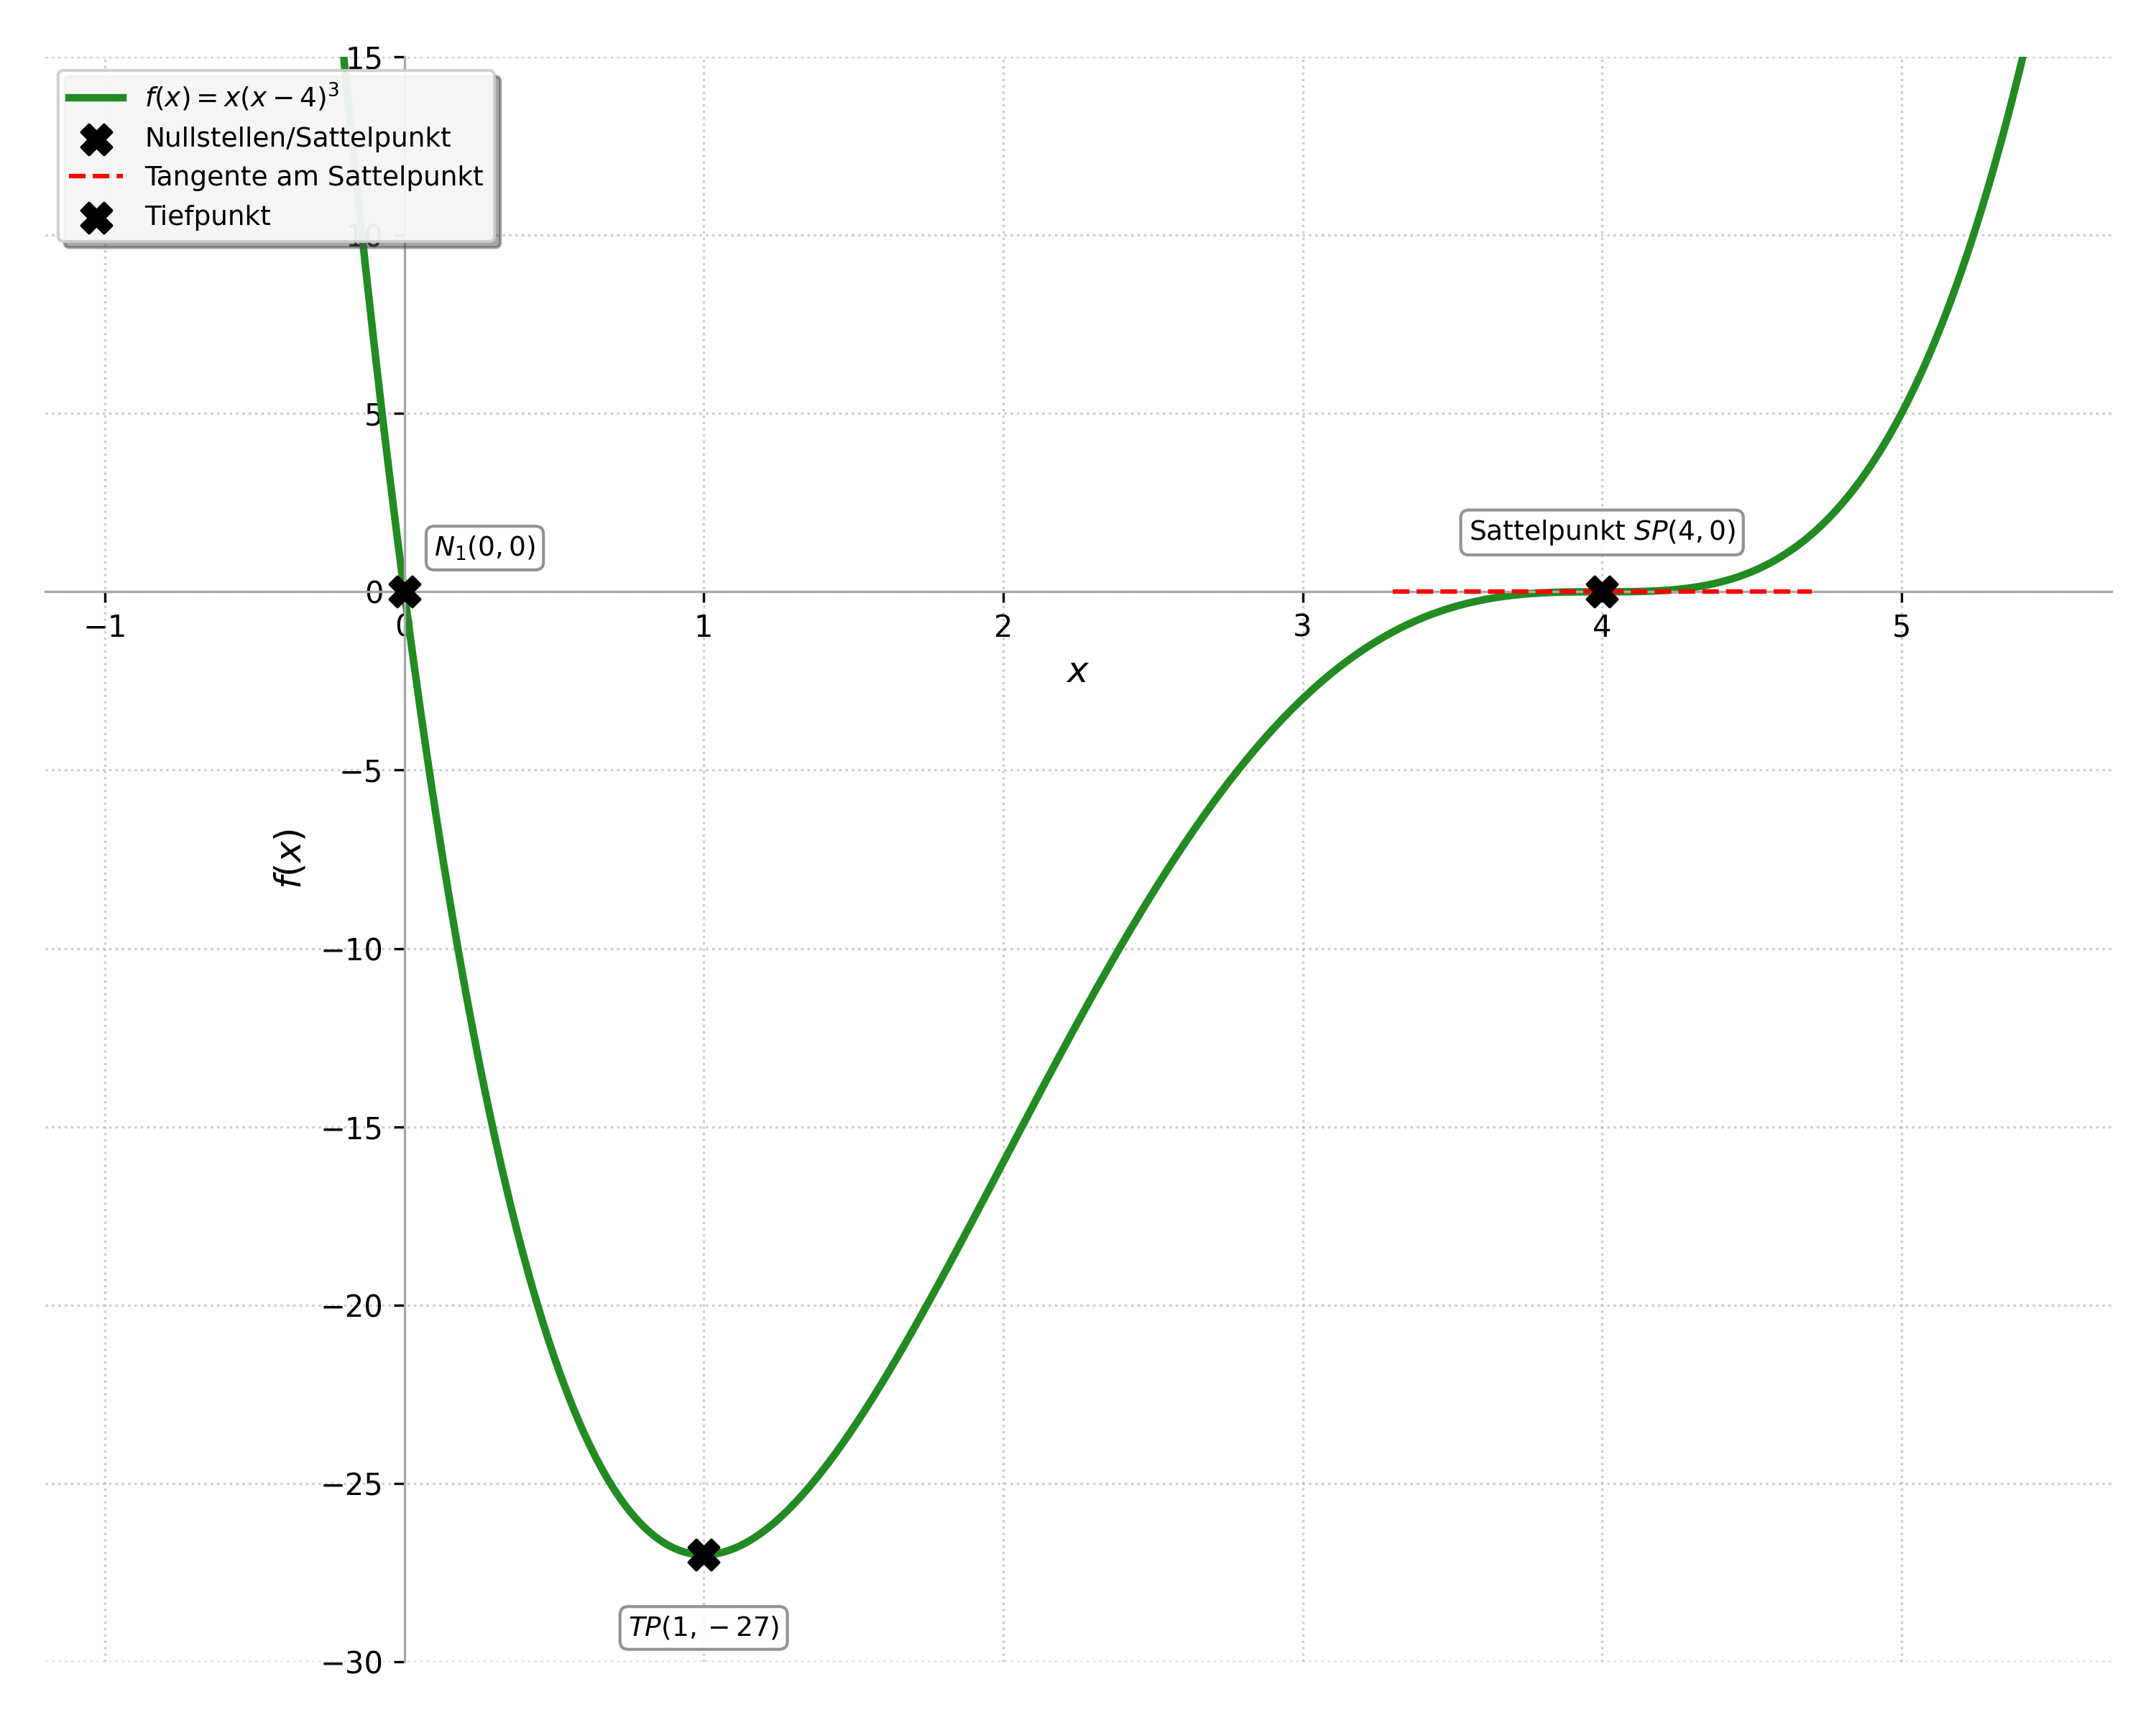
\includegraphics[width=0.8\textwidth]{grafiken/f_tueftler_produkt_kette_graph.png}
        % --- Beschreibung der Skizze ---
        % Die Skizze zeigt den Graphen eines Polynoms 4. Grades.
        % Nullstellen: (0|0) - Schnittpunkt; (4|0) - Sattelpunkt (berührt und durchdringt x-Achse mit horizontaler Tangente).
        % Lokaler Tiefpunkt: (1|-27).
        % Verlauf: Kommt von links oben, fällt zum TP(1|-27), steigt zum SP(4|0), steigt dann weiter nach rechts oben.
        \captionof{figure}{Graph der Funktion $f(x) = x(x-4)^3$.}
        \label{fig:f_tueftler_produkt_kette_graph}
        \end{center}
    \end{itemize}
\end{enumerate}

\end{loesungsumgebung}

\begin{aufgabenumgebung}{Optimierungsproblem – Die optimale Schachtel}
Aus einem quadratischen Stück Pappe der Seitenlänge $L=30\,$cm soll durch Ausschneiden von Quadraten an den Ecken und anschließendes Hochbiegen der entstehenden Seitenlaschen eine offene Schachtel (ohne Deckel) mit maximalem Volumen hergestellt werden.


\begin{enumerate}
    \item \textbf{Variable festlegen:} Sei $x$ die Seitenlänge der Quadrate, die an den Ecken ausgeschnitten werden.
    \item \textbf{Maße der Schachtel:} Drücke die Länge $l$, die Breite $b$ und die Höhe $h$ der entstehenden Schachtel in Abhängigkeit von $x$ aus. Bedenke, dass von jeder Seite der Pappe $2x$ weggeschnitten wird.
    \item \textbf{Definitionsbereich für $x$:} Welche Werte für $x$ sind in diesem Sachzusammenhang sinnvoll? (Die Seitenlängen müssen positiv sein, und man kann nicht mehr wegschneiden, als Pappe da ist).
    \item \textbf{Zielfunktion für das Volumen:} Stelle die Funktion $V(x)$ auf, die das Volumen der Schachtel in Abhängigkeit von $x$ beschreibt ($V = l \cdot b \cdot h$).
    \item \textbf{Extremwertsuche:}
        \begin{itemize}
            \item Bilde die erste Ableitung $V'(x)$.
            \item Setze $V'(x)=0$ und löse nach $x$, um die kritischen Stellen zu finden.
            \item Überprüfe mit der zweiten Ableitung $V''(x)$ (oder dem Vorzeichenwechselkriterium von $V'(x)$), ob an den kritischen Stellen ein Maximum oder Minimum vorliegt.
            \item Berücksichtige den Definitionsbereich von $x$: Liegen die gefundenen Extremstellen im sinnvollen Bereich?
        \end{itemize}
    \item \textbf{Antwort:} Gib die Seitenlänge $x$ der auszuschneidenden Quadrate an, für die das Volumen der Schachtel maximal wird, sowie das maximale Volumen selbst.
\end{enumerate}
\end{aufgabenumgebung}

\begin{loesungsumgebung}[loes:optimierung-schachtel]{Optimierungsproblem – Die optimale Schachtel}

\begin{enumerate}
    \item \textbf{Variable festlegen:}
    Sei $x$ die Seitenlänge der Quadrate (in cm), die an den Ecken des quadratischen Stücks Pappe ausgeschnitten werden. Diese Seitenlänge $x$ wird dann auch die Höhe der entstehenden Schachtel sein.

    \item \textbf{Maße der Schachtel:}
    Die ursprüngliche Pappe hat eine Seitenlänge von $L=30\,$cm. Wenn an jeder Ecke ein Quadrat der Seitenlänge $x$ ausgeschnitten wird, verringert sich jede Seite der entstehenden Grundfläche um $2x$.
    \begin{itemize}
        \item Höhe der Schachtel: $h = x$.
        \item Länge der Grundfläche: $l = L - 2x = 30 - 2x$.
        \item Breite der Grundfläche: $b = L - 2x = 30 - 2x$.
    \end{itemize}

    \item \textbf{Definitionsbereich für $x$:}
    Damit eine Schachtel entstehen kann, muss $x$ positiv sein: $x > 0$.
    Außerdem müssen die Seitenlängen der Grundfläche positiv sein: $30 - 2x > 0$.
    $30 > 2x \Rightarrow 15 > x$.
    Zusammenfassend muss $0 < x < 15$ gelten. Der sinnvolle Definitionsbereich für $x$ ist also das offene Intervall $\mathbf{(0, 15)}$ cm.

    \item \textbf{Zielfunktion für das Volumen:}
    Das Volumen $V$ einer Schachtel ist $V = l \cdot b \cdot h$.
    $V(x) = (30-2x) \cdot (30-2x) \cdot x = (30-2x)^2 x$.
    Ausmultipliziert ergibt sich:
    $V(x) = (900 - 120x + 4x^2)x = \mathbf{4x^3 - 120x^2 + 900x}$.

    \item \textbf{Extremwertsuche:}
    \begin{itemize}
        \item \textbf{Erste Ableitung $V'(x)$ bilden:}
        $V'(x) = \frac{d}{dx}(4x^3 - 120x^2 + 900x) = 12x^2 - 240x + 900$.
        \item \textbf{Kritische Stellen finden ($V'(x)=0$):}
        $12x^2 - 240x + 900 = 0$.
        Wir teilen die Gleichung durch 12:
        $x^2 - 20x + 75 = 0$.
        Mit der p-q-Formel ($p=-20, q=75$):
        $x_{1,2} = - \frac{-20}{2} \pm \sqrt{\left(\frac{-20}{2}\right)^2 - 75}$
        $x_{1,2} = 10 \pm \sqrt{(-10)^2 - 75}$
        $x_{1,2} = 10 \pm \sqrt{100 - 75}$
        $x_{1,2} = 10 \pm \sqrt{25}$
        $x_{1,2} = 10 \pm 5$.
        Die kritischen Stellen sind $x_1 = 10 + 5 = 15$ und $x_2 = 10 - 5 = 5$.
        \item \textbf{Überprüfung mit der zweiten Ableitung $V''(x)$:}
        $V''(x) = \frac{d}{dx}(12x^2 - 240x + 900) = 24x - 240$.
        Für $x_1 = 15$: $V''(15) = 24(15) - 240 = 360 - 240 = 120$.
        Da $V''(15) > 0$, liegt bei $x=15$ ein lokales Minimum vor.
        Für $x_2 = 5$: $V''(5) = 24(5) - 240 = 120 - 240 = -120$.
        Da $V''(5) < 0$, liegt bei $x=5$ ein lokales Maximum vor.
        \item \textbf{Berücksichtigung des Definitionsbereichs von $x$:}
        Der Definitionsbereich ist $(0, 15)$.
        Die kritische Stelle $x_1=15$ liegt nicht im offenen Definitionsbereich (hier wäre die Grundfläche Null).
        Die kritische Stelle $x_2=5$ liegt im Definitionsbereich $(0,15)$. Da es sich um ein lokales Maximum handelt und an den Rändern des Definitionsbereichs das Volumen gegen Null geht ($V(x) \to 0$ für $x \to 0^+$ und $V(x) = 0$ für $x=15$), ist dies das globale Maximum im sinnvollen Bereich.
    \end{itemize}

    \item \textbf{Antwort:}
    Die Seitenlänge $x$ der auszuschneidenden Quadrate, für die das Volumen der Schachtel maximal wird, ist $\mathbf{x = 5\,cm}$.
    Das maximale Volumen beträgt:
    $V(5) = (30-2(5))^2 \cdot 5 = (30-10)^2 \cdot 5 = (20)^2 \cdot 5 = 400 \cdot 5 = \mathbf{2000\,cm^3}$.
    Die Abmessungen der Schachtel mit maximalem Volumen sind:
    \begin{itemize}
        \item Höhe: $h = x = 5\,$cm.
        \item Länge der Grundfläche: $l = 30 - 2(5) = 20\,$cm.
        \item Breite der Grundfläche: $b = 30 - 2(5) = 20\,$cm.
    \end{itemize}
\end{enumerate}

\end{loesungsumgebung}

\begin{aufgabenumgebung}{Rekonstruktion einer Polynomfunktion}
Eine ganzrationale Funktion dritten Grades $f(x) = ax^3 + bx^2 + cx + d$ hat die folgenden Eigenschaften:
\begin{itemize}
    \item Der Graph der Funktion geht durch den Ursprung $P(0|0)$.
    \item Der Ursprung ist gleichzeitig ein Wendepunkt der Funktion.
    \item Die Tangente im Wendepunkt (die Wendetangente) hat die Gleichung $y_W(x) = -3x$.
    \item Der Graph der Funktion hat eine Nullstelle bei $x_N = 1$.
\end{itemize}
Bestimme die Funktionsgleichung $f(x)$.



\end{aufgabenumgebung}


\begin{loesungsumgebung}[loes:rekonstruktion-polynom3]{Rekonstruktion einer Polynomfunktion}
Die allgemeine Form der gesuchten ganzrationalen Funktion dritten Grades ist $f(x) = ax^3 + bx^2 + cx + d$.
Ihre Ableitungen lauten:
$f'(x) = 3ax^2 + 2bx + c$
$f''(x) = 6ax + 2b$

Wir übersetzen die gegebenen Eigenschaften in Gleichungen:

\begin{itemize}
    \item \textbf{Der Graph der Funktion geht durch den Ursprung $P(0|0)$:} \\
    Diese Bedingung bedeutet $f(0)=0$.
    $f(0) = a(0)^3 + b(0)^2 + c(0) + d = 0 \Rightarrow \mathbf{d=0}$. (Gleichung 1)

    \item \textbf{Der Ursprung ist gleichzeitig ein Wendepunkt der Funktion:} \\
    Ein Wendepunkt liegt an der Stelle $x_W=0$. Notwendige Bedingung für einen Wendepunkt ist $f''(x_W)=0$.
    $f''(0) = 6a(0) + 2b = 0 \Rightarrow 2b=0 \Rightarrow \mathbf{b=0}$. (Gleichung 2)
    (Hinweis: Damit es tatsächlich ein Wendepunkt ist, müsste $f'''(0) \neq 0$ sein. $f'''(x)=6a$. Wenn $a \neq 0$, ist diese Bedingung erfüllt.)

    \item \textbf{Die Tangente im Wendepunkt (Ursprung) hat die Gleichung $y_W(x) = -3x$:} \\
    Der Wendepunkt ist $W(0|0)$. Die Steigung der Wendetangente ist die Ableitung $f'(x_W)$ an der Wendestelle $x_W=0$. Die gegebene Tangentengleichung $y_W(x)=-3x$ hat die Steigung $m_W=-3$.
    Also $f'(0) = -3$.
    $f'(0) = 3a(0)^2 + 2b(0) + c = -3 \Rightarrow \mathbf{c=-3}$. (Gleichung 3)

    \item \textbf{Der Graph der Funktion hat eine Nullstelle bei $x_N = 1$:} \\
    Diese Bedingung bedeutet $f(1)=0$.
    $f(1) = a(1)^3 + b(1)^2 + c(1) + d = 0 \Rightarrow a+b+c+d=0$. (Gleichung 4)
\end{itemize}

\textbf{Lösen des Gleichungssystems:}
Wir haben bereits direkt erhalten:
\begin{itemize}
    \item $d=0$ (aus Gleichung 1)
    \item $b=0$ (aus Gleichung 2)
    \item $c=-3$ (aus Gleichung 3)
\end{itemize}
Diese Werte setzen wir in Gleichung 4 ein:
$a + b + c + d = 0$
$a + 0 + (-3) + 0 = 0$
$a - 3 = 0 \Rightarrow \mathbf{a=3}$.

Die Koeffizienten der Funktion sind also $a=3, b=0, c=-3, d=0$.

\textbf{Funktionsgleichung:}
Die gesuchte Funktionsgleichung lautet:
$f(x) = 3x^3 + 0x^2 - 3x + 0$
$$ \mathbf{f(x) = 3x^3 - 3x} $$

\textbf{Überprüfung (optional):}
\begin{itemize}
    \item $f(0) = 3(0)^3 - 3(0) = 0$. (Punkt $P(0|0)$ liegt auf dem Graphen)
    \item $f'(x) = 9x^2 - 3$, $f''(x) = 18x$, $f'''(x) = 18$.
    \item $f''(0) = 18(0) = 0$. $f'''(0) = 18 \neq 0$. Also ist bei $x=0$ ein Wendepunkt.
    \item $f'(0) = 9(0)^2 - 3 = -3$. Die Steigung der Wendetangente im Ursprung ist $-3$, die Tangente ist $y=-3x$.
    \item $f(1) = 3(1)^3 - 3(1) = 3-3=0$. (Nullstelle bei $x=1$)
\end{itemize}
Alle Bedingungen sind erfüllt.
\end{loesungsumgebung}


\begin{aufgabenumgebung}{Bewegungsanalyse – Zwei Läufer auf der Bahn}
Zwei Läufer, A und B, bewegen sich auf einer geraden Bahn.
Läufer A startet zum Zeitpunkt $t=0\,$s am Punkt $s_A(0)=0\,$m. Seine Position (in Metern) zum Zeitpunkt $t$ (in Sekunden) wird durch die Funktion $s_A(t) = t^2$ beschrieben.
Läufer B startet gleichzeitig am Punkt $s_B(0)=10\,$m. Seine Position wird durch $s_B(t) = -0.5t^2 + 7t + 10$ beschrieben.
Wir betrachten das Zeitintervall $[0, 5]$ Sekunden.

\begin{enumerate}
    \item \textbf{Geschwindigkeiten:} Bestimme die Geschwindigkeitsfunktionen $v_A(t) = s_A'(t)$ und $v_B(t) = s_B'(t)$ der beiden Läufer.
    \item \textbf{Gleiche Geschwindigkeit:} Zu welchem Zeitpunkt $t$ haben beide Läufer die gleiche Geschwindigkeit? Wie groß ist diese Geschwindigkeit?
    \item \textbf{Gleiche Position:} Haben die Läufer jemals die gleiche Position im betrachteten Zeitintervall $[0,5]$? Wenn ja, zu welchem Zeitpunkt/welchen Zeitpunkten?
    \item \textbf{Abstand der Läufer:}
        \begin{itemize}
            \item Stelle eine Funktion $d(t)$ auf, die den Abstand zwischen den beiden Läufern zum Zeitpunkt $t$ beschreibt. 
            \textit{Hinweis:} Überlege zuerst, welcher Läufer im Intervall $[0,5]$ vorne liegt, um das Betragszeichen bei der Differenz $d(t) = |s_B(t) - s_A(t)|$ auflösen zu können. Du hast in Teil c) untersucht, ob sie sich treffen.
            \item Zu welchem Zeitpunkt im Intervall $[0,5]$ ist der Abstand zwischen den Läufern minimal? Wie groß ist dieser minimale Abstand?
            \item Zu welchem Zeitpunkt im Intervall $[0,5]$ ist der Abstand zwischen den Läufern maximal? Wie groß ist dieser maximale Abstand?
        \end{itemize}
\end{enumerate}
\end{aufgabenumgebung}


\begin{loesungsumgebung}[loes:bewegung-zwei-laeufer]{Bewegungsanalyse – Zwei Läufer auf der Bahn}
Wir analysieren die Bewegung der Läufer A und B im Zeitintervall $[0, 5]$ Sekunden.
Die Positionen sind gegeben durch $s_A(t) = t^2$ und $s_B(t) = -0.5t^2 + 7t + 10$.

\begin{enumerate}[label=(\alph*)]
    \item \textbf{Geschwindigkeiten:}
    Die Geschwindigkeitsfunktionen sind die ersten Ableitungen der Ortsfunktionen:
    \begin{itemize}
        \item Für Läufer A: $v_A(t) = s_A'(t) = \frac{d}{dt}(t^2) = \mathbf{2t}$ (m/s).
        \item Für Läufer B: $v_B(t) = s_B'(t) = \frac{d}{dt}(-0.5t^2 + 7t + 10) = -0.5 \cdot 2t + 7 = \mathbf{-t + 7}$ (m/s).
    \end{itemize}

    \item \textbf{Gleiche Geschwindigkeit:}
    Wir setzen $v_A(t) = v_B(t)$:
    $2t = -t + 7$
    $$
    \begin{array}{r c l c l}
    \umformung{2t}{-t+7}{+}{t}
    \umformung{3t}{7}{\div}{3}
    \umformungend{t}{7/3}
    \end{array}
    $$
    Zum Zeitpunkt $\mathbf{t = \frac{7}{3}\,s \approx 2.33\,s}$ haben beide Läufer die gleiche Geschwindigkeit.
    Diese Geschwindigkeit beträgt:
    $v_A(\frac{7}{3}) = 2 \cdot \frac{7}{3} = \frac{14}{3}\,$m/s.
    $v_B(\frac{7}{3}) = -\frac{7}{3} + 7 = -\frac{7}{3} + \frac{21}{3} = \frac{14}{3}\,$m/s.
    Die gemeinsame Geschwindigkeit ist $\mathbf{\frac{14}{3}\,m/s \approx 4.67\,m/s}$.

    \item \textbf{Gleiche Position:}
    Wir setzen $s_A(t) = s_B(t)$:
    $t^2 = -0.5t^2 + 7t + 10$
    $1.5t^2 - 7t - 10 = 0$.
    Multiplikation mit 2 ergibt: $3t^2 - 14t - 20 = 0$.
    Wir verwenden die Mitternachtsformel $t_{1,2} = \frac{-b \pm \sqrt{b^2-4ac}}{2a}$ mit $a=3, b=-14, c=-20$:
    $D = (-14)^2 - 4(3)(-20) = 196 + 240 = 436$.
    $t_{1,2} = \frac{14 \pm \sqrt{436}}{2 \cdot 3} = \frac{14 \pm 2\sqrt{109}}{6} = \frac{7 \pm \sqrt{109}}{3}$.
    $t_1 = \frac{7 + \sqrt{109}}{3} \approx \frac{7 + 10.440}{3} \approx \frac{17.440}{3} \approx 5.813\,$s.
    $t_2 = \frac{7 - \sqrt{109}}{3} \approx \frac{7 - 10.440}{3} \approx \frac{-3.440}{3} \approx -1.147\,$s.
    Der Zeitpunkt $t_1 \approx 5.813\,$s liegt außerhalb des Intervalls $[0,5]$. Der Zeitpunkt $t_2 \approx -1.147\,$s ist negativ und somit nicht relevant.
    Daher haben die Läufer im betrachteten Zeitintervall $[0,5]$ \textbf{niemals die gleiche Position}.

    \item \textbf{Abstand der Läufer:}
    \begin{itemize}
        \item \textbf{Abstandsfunktion $d(t)$:}
        Da sich die Läufer im Intervall $[0,5]$ nicht treffen und $s_A(0)=0$ sowie $s_B(0)=10$ ist ($s_B(0) > s_A(0)$), liegt Läufer B im gesamten Intervall $[0,5]$ vor Läufer A.
        Somit ist der Abstand $d(t) = s_B(t) - s_A(t)$.
        $d(t) = (-0.5t^2 + 7t + 10) - (t^2) = \mathbf{-1.5t^2 + 7t + 10}$.

        \item \textbf{Minimaler Abstand im Intervall $[0,5]$:}
        Um den minimalen Abstand zu finden, untersuchen wir die Extremwerte von $d(t)$ im Intervall $[0,5]$.
        $d'(t) = \frac{d}{dt}(-1.5t^2 + 7t + 10) = -3t + 7$.
        Kritische Stelle: $d'(t)=0 \Rightarrow -3t + 7 = 0 \Rightarrow 3t=7 \Rightarrow t = \frac{7}{3}$.
        $t = \frac{7}{3} \approx 2.33\,$s liegt im Intervall $[0,5]$.
        Zweite Ableitung: $d''(t) = -3$.
        Da $d''(\frac{7}{3}) = -3 < 0$, liegt bei $t=\frac{7}{3}\,$s ein lokales Maximum des Abstands vor.
        Der minimale Abstand muss also an den Rändern des Intervalls $[0,5]$ angenommen werden.
        $d(0) = -1.5(0)^2 + 7(0) + 10 = 10\,$m.
        $d(5) = -1.5(5)^2 + 7(5) + 10 = -1.5(25) + 35 + 10 = -37.5 + 35 + 10 = 7.5\,$m.
        Der minimale Abstand beträgt $\mathbf{7.5\,m}$ zum Zeitpunkt $\mathbf{t=5\,s}$.

        \item \textbf{Maximaler Abstand im Intervall $[0,5]$:}
        Wir vergleichen die Werte an den Rändern und am lokalen Extremum (welches hier ein Maximum ist):
        $d(0) = 10\,$m.
        $d(5) = 7.5\,$m.
        $d(\frac{7}{3}) = -1.5\left(\frac{7}{3}\right)^2 + 7\left(\frac{7}{3}\right) + 10 = -1.5\left(\frac{49}{9}\right) + \frac{49}{3} + 10$
        $d(\frac{7}{3}) = -\frac{3}{2} \cdot \frac{49}{9} + \frac{49}{3} + 10 = -\frac{49}{6} + \frac{98}{6} + \frac{60}{6} = \frac{-49+98+60}{6} = \frac{109}{6}$.
        $d(\frac{7}{3}) = \frac{109}{6} \approx 18.167\,$m.
        Der maximale Abstand beträgt $\mathbf{\frac{109}{6}\,m \approx 18.17\,m}$ zum Zeitpunkt $\mathbf{t=\frac{7}{3}\,s}$.
    \end{itemize}
\end{enumerate}

\end{loesungsumgebung}


\begin{aufgabenumgebung}{Tangentenprobleme an einer kubischen Funktion}
Gegeben ist die Funktion $f(x) = x^3 - 3x$.
\begin{enumerate}
    \item \textbf{Parallele Tangenten:}
        \begin{itemize}
            \item Bestimme die Steigung der Geraden $g(x) = 9x - 5$.
            \item Gibt es Punkte auf dem Graphen von $f(x)$, an denen die Tangente parallel zur Geraden $g(x)$ ist? Wenn ja, bestimme die Koordinaten dieser Punkte.
            \item Gib die Gleichungen der Tangenten an den Graphen von $f(x)$ in diesen Punkten an.
        \end{itemize}
    \item \textbf{Tangente von einem externen Punkt:}
        Von welchem Punkt $P_y(0|y_P)$ auf der y-Achse aus kann man eine Tangente an den Graphen von $f(x)$ legen, die den Graphen an der Stelle $x_B=2$ berührt?

\end{enumerate}
\end{aufgabenumgebung}

\begin{loesungsumgebung}[loes:tangentenprobleme-kubisch]{Tangentenprobleme an einer kubischen Funktion}
Gegeben ist die Funktion $f(x) = x^3 - 3x$. Ihre erste Ableitung ist $f'(x) = 3x^2 - 3$.

\begin{enumerate}[label=(\alph*)]
    \item \textbf{Parallele Tangenten:}
    \begin{itemize}
        \item \textbf{Steigung der Geraden $g(x) = 9x - 5$:}
        Die Steigung $m_g$ der Geraden $g(x)$ ist der Koeffizient von $x$, also $\mathbf{m_g = 9}$.

        \item \textbf{Punkte auf dem Graphen von $f(x)$, an denen die Tangente parallel zur Geraden $g(x)$ ist:}
        Parallelität bedeutet gleiche Steigung. Wir suchen also Stellen $x$, an denen $f'(x) = m_g = 9$ gilt.
        $3x^2 - 3 = 9$
        $$
        \begin{array}{r c l c l}
        \umformung{3x^2 - 3}{9}{+}{3}
        \umformung{3x^2}{12}{\div}{3}
        \umformungend{x^2}{4}
        \end{array}
        $$
        Aus $x^2=4$ folgt $x = \pm\sqrt{4}$, also $x_1 = 2$ und $x_2 = -2$.
        Dies sind die x-Koordinaten der gesuchten Punkte. Die y-Koordinaten sind:
        $f(2) = (2)^3 - 3(2) = 8 - 6 = 2$. Punkt $\mathbf{P_1(2|2)}$.
        $f(-2) = (-2)^3 - 3(-2) = -8 + 6 = -2$. Punkt $\mathbf{P_2(-2|-2)}$.

        \item \textbf{Gleichungen der Tangenten an den Graphen von $f(x)$ in diesen Punkten:}
        Die Steigung beider Tangenten ist $m_t = 9$.
        \begin{itemize}
            \item Tangente $t_1$ im Punkt $P_1(2|2)$:
            $y - y_1 = m_t(x - x_1)$
            $y - 2 = 9(x - 2)$
            $y = 9x - 18 + 2$
            $\mathbf{t_1(x): y = 9x - 16}$.
            \item Tangente $t_2$ im Punkt $P_2(-2|-2)$:
            $y - y_2 = m_t(x - x_2)$
            $y - (-2) = 9(x - (-2))$
            $y + 2 = 9(x + 2)$
            $y = 9x + 18 - 2$
            $\mathbf{t_2(x): y = 9x + 16}$.
        \end{itemize}
    \end{itemize}

    \item \textbf{Tangente von einem externen Punkt:}
    Gesucht ist der Punkt $P_y(0|y_P)$ auf der y-Achse, von dem aus eine Tangente an $f(x)$ den Graphen an der Stelle $x_B=2$ berührt.
    \begin{enumerate}[label=\arabic*.]
        \item \textbf{Bestimme die y-Koordinate des Berührpunkts $B(2|f(2))$:}
        $f(2) = (2)^3 - 3(2) = 8 - 6 = 2$.
        Der Berührpunkt ist $\mathbf{B(2|2)}$.

        \item \textbf{Bestimme die Steigung $m_T$ der Tangente an $f(x)$ an der Stelle $x_B=2$:}
        $m_T = f'(x_B) = f'(2) = 3(2)^2 - 3 = 3(4) - 3 = 12 - 3 = \mathbf{9}$.

        \item \textbf{Stelle die Gleichung der Tangente $t_B(x)$ im Punkt $B$ auf:}
        Mit dem Punkt $B(2|2)$ und der Steigung $m_T=9$:
        $y - 2 = 9(x - 2)$
        $y = 9x - 18 + 2$
        $\mathbf{t_B(x): y = 9x - 16}$.

        \item \textbf{Der gesuchte Punkt $P_y(0|y_P)$ muss auf dieser Tangente $t_B(x)$ liegen:}
        Setze $x=0$ in die Tangentengleichung $y = 9x - 16$ ein, um $y_P$ zu finden:
        $y_P = 9(0) - 16 = -16$.
        Der gesuchte Punkt auf der y-Achse ist $\mathbf{P_y(0|-16)}$.
    \end{enumerate}
\end{enumerate}

\end{loesungsumgebung}


\begin{aufgabenumgebung}{Checkliste: Von kubischen Funktionen zu linearen Ableitungen}
Diese Aufgabe zeigt dir, wie dein Wissen über lineare Funktionen dir hilft, das Verhalten von Polynomen 3. Grades zu verstehen.
Betrachte die Funktion $f(x) = x^3 - 6x^2 + 10x - 3$.

\begin{enumerate}[label=(\alph*)]
    \item \textbf{Ableitungen bilden:} Berechne die erste Ableitung $f'(x)$ und die zweite Ableitung $f''(x)$ der Funktion $f(x)$.
    \item \textbf{Analyse der zweiten Ableitung:}
    \begin{itemize}
        \item Welchen Funktionstyp erkennst du in $f''(x)$? Gib die Steigung $m_{f''}$ und den y-Achsenabschnitt $c_{f''}$ dieser Funktion an.
        \item Berechne die Nullstelle $x_W$ von $f''(x)$. Welche besondere Bedeutung hat diese Stelle $x_W$ für den Graphen der ursprünglichen Funktion $f(x)$? (Erinnere dich an die Definition von Wendepunkten).
    \end{itemize}
    \item \textbf{Krümmungsverhalten von $f(x)$ bestimmen:}
    Nutze dein Wissen über lineare Funktionen, um das Vorzeichen von $f''(x)$ zu bestimmen:
    \begin{itemize}
        \item Für welche $x$-Werte ist $f''(x) > 0$? (Tipp: Wann sind die Werte einer steigenden/fallenden linearen Funktion positiv?)
        \item Für welche $x$-Werte ist $f''(x) < 0$?
        \item Welche Schlussfolgerungen ziehst du daraus für das Krümmungsverhalten (links- oder rechtsgekrümmt) des Graphen von $f(x)$? Gib die Intervalle an.
    \end{itemize}
    \item \textbf{Reflexion:} Erkläre in eigenen Worten, warum das Verständnis der Eigenschaften einer linearen Funktion (insbesondere ihrer Nullstelle und des Vorzeichenverlaufs in Abhängigkeit von der Steigung) nützlich ist, um das Krümmungsverhalten einer kubischen Funktion zu analysieren.
\end{enumerate}
\end{aufgabenumgebung}


\begin{loesungsumgebung}[loes:kubisch-zu-linear-ableitung]{Checkliste: Von kubischen Funktionen zu linearen Ableitungen}
Wir betrachten die Funktion $f(x) = x^3 - 6x^2 + 10x - 3$.

\begin{enumerate}[label=(\alph*)]
    \item \textbf{Ableitungen bilden:}
    \begin{itemize}
        \item Erste Ableitung $f'(x)$:
        $$ f'(x) = \frac{d}{dx}(x^3 - 6x^2 + 10x - 3) = \mathbf{3x^2 - 12x + 10} $$
        \item Zweite Ableitung $f''(x)$:
        $$ f''(x) = \frac{d}{dx}(3x^2 - 12x + 10) = \mathbf{6x - 12} $$
    \end{itemize}

    \item \textbf{Analyse der zweiten Ableitung $f''(x) = 6x - 12$:}
    \begin{itemize}
        \item \textbf{Funktionstyp, Steigung und y-Achsenabschnitt:}
        $f''(x)$ ist eine \textbf{lineare Funktion}.
        Ihre Steigung ist $m_{f''} = 6$.
        Ihr y-Achsenabschnitt ist $c_{f''} = -12$ (denn $f''(0) = -12$).
        \item \textbf{Nullstelle $x_W$ von $f''(x)$ und ihre Bedeutung:}
        Wir setzen $f''(x_W) = 0$:
        $6x_W - 12 = 0$
        $6x_W = 12$
        $x_W = 2$.
        Die Nullstelle der zweiten Ableitung ist $\mathbf{x_W = 2}$.
        Diese Stelle $x_W$ ist eine \textbf{potentielle Wendestelle} für die ursprüngliche Funktion $f(x)$. Um dies zu bestätigen, prüfen wir die dritte Ableitung:
        $f'''(x) = \frac{d}{dx}(6x - 12) = 6$.
        Da $f'''(2) = 6 \neq 0$, liegt bei $x_W=2$ tatsächlich ein Wendepunkt von $f(x)$ vor.
    \end{itemize}

    \item \textbf{Krümmungsverhalten von $f(x)$ bestimmen:}
    Das Krümmungsverhalten von $f(x)$ wird durch das Vorzeichen von $f''(x) = 6x - 12$ bestimmt.
    Da $f''(x)$ eine lineare Funktion mit positiver Steigung ($m_{f''} = 6 > 0$) und einer Nullstelle bei $x_W=2$ ist, gilt:
    \begin{itemize}
        \item \textbf{Für welche $x$-Werte ist $f''(x) > 0$?}
        Eine steigende lineare Funktion ist rechts von ihrer Nullstelle positiv.
        Also ist $f''(x) > 0$ für $\mathbf{x > 2}$.
        \item \textbf{Für welche $x$-Werte ist $f''(x) < 0$?}
        Eine steigende lineare Funktion ist links von ihrer Nullstelle negativ.
        Also ist $f''(x) < 0$ für $\mathbf{x < 2}$.
        \item \textbf{Schlussfolgerungen für das Krümmungsverhalten von $f(x)$:}
        \begin{itemize}
            \item Im Intervall $(-\infty, 2)$ ist $f''(x) < 0$, daher ist der Graph von $f(x)$ hier \textbf{rechtsgekrümmt} (konkav).
            \item Im Intervall $(2, \infty)$ ist $f''(x) > 0$, daher ist der Graph von $f(x)$ hier \textbf{linksgekrümmt} (konvex).
        \end{itemize}
        Bei $x=2$ findet ein Wechsel des Krümmungsverhaltens statt, was den Wendepunkt bestätigt.
    \end{itemize}

    \item \textbf{Reflexion:}
    Die zweite Ableitung $f''(x)$ einer kubischen Funktion $f(x)$ ist stets eine lineare Funktion. Die Analyse dieser linearen Funktion $f''(x)$ ist entscheidend für das Verständnis des Krümmungsverhaltens der kubischen Funktion $f(x)$:
    \begin{itemize}
        \item Die \textbf{Nullstelle $x_W$ der linearen Funktion $f''(x)$} gibt die x-Koordinate des Wendepunkts der kubischen Funktion $f(x)$ an. An dieser Stelle ändert $f(x)$ sein Krümmungsverhalten.
        \item Das \textbf{Vorzeichen der linearen Funktion $f''(x)$} bestimmt die Krümmungsrichtung von $f(x)$:
        \begin{itemize}
            \item Ist $f''(x) > 0$, so ist $f(x)$ linksgekrümmt.
            \item Ist $f''(x) < 0$, so ist $f(x)$ rechtsgekrümmt.
        \end{itemize}
        \item Die \textbf{Steigung der linearen Funktion $f''(x)$} (also der Koeffizient von $x$ in $f''(x)$ bzw. der Wert $f'''(x)$) gibt an, wie sich die Krümmung ändert. Ist die Steigung von $f''(x)$ positiv, so wechselt $f''(x)$ an seiner Nullstelle von negativen zu positiven Werten, was für $f(x)$ einen Übergang von Rechts- zu Linkskrümmung bedeutet. Ist die Steigung von $f''(x)$ negativ, ist es umgekehrt.
    \end{itemize}
    Indem man also die Eigenschaften einer einfachen linearen Funktion (ihre Nullstelle und wie ihr Vorzeichen von der Steigung abhängt) versteht, kann man direkt auf das komplexere Krümmungsverhalten einer kubischen Funktion schließen. Dies vereinfacht die Analyse erheblich.
\end{enumerate}

\end{loesungsumgebung}

\begin{aufgabenumgebung}{Checkliste: Von Polynomen 4. Grades zu quadratischen Ableitungen}
Diese Aufgabe zeigt dir, wie dein Wissen über quadratische Funktionen dir hilft, das Verhalten von Polynomen 4. Grades zu verstehen.
Betrachte die Funktion $g(x) = \frac{1}{4}x^4 - x^3 + x^2 + 1$.

\begin{enumerate}[label=(\alph*)]
    \item \textbf{Ableitungen bilden:} Berechne die erste Ableitung $g'(x)$ und die zweite Ableitung $g''(x)$ der Funktion $g(x)$.
    \item \textbf{Analyse der zweiten Ableitung:}
    \begin{itemize}
        \item Welchen Funktionstyp erkennst du in $g''(x)$? Gib die Parameter dieser Funktion an (z.B. Öffnungsfaktor, etc.). Ist der Graph von $g''(x)$ nach oben oder unten geöffnet?
        \item Berechne die Nullstellen $x_{W1}, x_{W2}$ von $g''(x)$ (falls vorhanden). Welche Bedeutung haben diese Stellen für den Graphen von $g(x)$?
    \end{itemize}
    \item \textbf{Krümmungsverhalten von $g(x)$ bestimmen:}
    Nutze dein Wissen über quadratische Funktionen, um das Vorzeichen von $g''(x)$ zu bestimmen:
    \begin{itemize}
        \item Skizziere (oder stelle dir vor) den Graphen von $g''(x)$ basierend auf Öffnungsrichtung und Nullstellen.
        \item Für welche $x$-Werte ist $g''(x) > 0$?
        \item Für welche $x$-Werte ist $g''(x) < 0$?
        \item Welche Schlussfolgerungen ziehst du daraus für das Krümmungsverhalten des Graphen von $g(x)$? Gib die Intervalle an. Wie viele Wendepunkte hat $g(x)$?
    \end{itemize}
    \item \textbf{Reflexion:} Erkläre, wie das Verständnis der Eigenschaften einer quadratischen Funktion (Öffnung, Nullstellen, Vorzeichenverlauf) hilft, das Krümmungsverhalten eines Polynoms 4. Grades zu analysieren.
\end{enumerate}
\end{aufgabenumgebung}


\begin{loesungsumgebung}[loes:polynom4-zu-quadrat-ableitung]{Checkliste: Von Polynomen 4. Grades zu quadratischen Ableitungen}
Wir betrachten die Funktion $g(x) = \frac{1}{4}x^4 - x^3 + x^2 + 1$.

\begin{enumerate}[label=(\alph*)]
    \item \textbf{Ableitungen bilden:}
    \begin{itemize}
        \item Erste Ableitung $g'(x)$:
        $$ g'(x) = \frac{d}{dx}\left(\frac{1}{4}x^4 - x^3 + x^2 + 1\right) = \frac{1}{4} \cdot 4x^3 - 3x^2 + 2x + 0 = \mathbf{x^3 - 3x^2 + 2x} $$
        \item Zweite Ableitung $g''(x)$:
        $$ g''(x) = \frac{d}{dx}(x^3 - 3x^2 + 2x) = \mathbf{3x^2 - 6x + 2} $$
    \end{itemize}

    \item \textbf{Analyse der zweiten Ableitung $g''(x) = 3x^2 - 6x + 2$:}
    \begin{itemize}
        \item \textbf{Funktionstyp, Parameter und Öffnung:}
        $g''(x)$ ist eine \textbf{quadratische Funktion}.
        Die Parameter in der Form $ax^2+bx+c$ sind $a_{g''} = 3$, $b_{g''} = -6$, $c_{g''} = 2$.
        Da der Öffnungsfaktor $a_{g''} = 3 > 0$ ist, ist der Graph von $g''(x)$ eine \textbf{nach oben geöffnete Parabel}.
        \item \textbf{Nullstellen $x_{W1}, x_{W2}$ von $g''(x)$ und ihre Bedeutung:}
        Wir setzen $g''(x_W) = 0$: $3x_W^2 - 6x_W + 2 = 0$.
        Mit der Mitternachtsformel (ABC-Formel):
        $x_W = \frac{-(-6) \pm \sqrt{(-6)^2 - 4(3)(2)}}{2(3)} = \frac{6 \pm \sqrt{36 - 24}}{6} = \frac{6 \pm \sqrt{12}}{6}$.
        Da $\sqrt{12} = \sqrt{4 \cdot 3} = 2\sqrt{3}$, erhalten wir:
        $x_W = \frac{6 \pm 2\sqrt{3}}{6} = 1 \pm \frac{2\sqrt{3}}{6} = 1 \pm \frac{\sqrt{3}}{3}$.
        Die potentiellen Wendestellen sind $\mathbf{x_{W1} = 1 - \frac{\sqrt{3}}{3} \approx 0.423}$ und $\mathbf{x_{W2} = 1 + \frac{\sqrt{3}}{3} \approx 1.577}$.
        Diese Stellen sind Kandidaten für Wendepunkte des Graphen der ursprünglichen Funktion $g(x)$.
        Um dies zu bestätigen, bilden wir $g'''(x) = \frac{d}{dx}(3x^2 - 6x + 2) = 6x - 6$.
        Für $x_{W1} = 1 - \frac{\sqrt{3}}{3}$: $g'''(1 - \frac{\sqrt{3}}{3}) = 6(1 - \frac{\sqrt{3}}{3}) - 6 = 6 - 2\sqrt{3} - 6 = -2\sqrt{3} \neq 0$.
        Für $x_{W2} = 1 + \frac{\sqrt{3}}{3}$: $g'''(1 + \frac{\sqrt{3}}{3}) = 6(1 + \frac{\sqrt{3}}{3}) - 6 = 6 + 2\sqrt{3} - 6 = 2\sqrt{3} \neq 0$.
        Da $g'''(x_W) \neq 0$ an beiden Stellen, sind dies tatsächlich Wendestellen von $g(x)$.
    \end{itemize}

    \item \textbf{Krümmungsverhalten von $g(x)$ bestimmen:}
    Das Krümmungsverhalten von $g(x)$ wird durch das Vorzeichen von $g''(x) = 3x^2 - 6x + 2$ bestimmt.
    \begin{itemize}
        \item \textbf{Skizze/Vorstellung des Graphen von $g''(x)$:}
        Der Graph von $g''(x)$ ist eine nach oben geöffnete Parabel, die die x-Achse an den Stellen $x_{W1} = 1 - \frac{\sqrt{3}}{3}$ und $x_{W2} = 1 + \frac{\sqrt{3}}{3}$ schneidet.
        \item \textbf{Für welche $x$-Werte ist $g''(x) > 0$?}
        Eine nach oben geöffnete Parabel ist außerhalb ihrer Nullstellen positiv.
        Also ist $g''(x) > 0$ für $\mathbf{x < 1 - \frac{\sqrt{3}}{3}}$ oder $\mathbf{x > 1 + \frac{\sqrt{3}}{3}}$.
        \item \textbf{Für welche $x$-Werte ist $g''(x) < 0$?}
        Eine nach oben geöffnete Parabel ist zwischen ihren Nullstellen negativ.
        Also ist $g''(x) < 0$ für $\mathbf{1 - \frac{\sqrt{3}}{3} < x < 1 + \frac{\sqrt{3}}{3}}$.
        \item \textbf{Schlussfolgerungen für das Krümmungsverhalten von $g(x)$ und Anzahl Wendepunkte:}
        \begin{itemize}
            \item Im Intervall $(-\infty, 1 - \frac{\sqrt{3}}{3})$ ist $g''(x) > 0 \Rightarrow g(x)$ ist \textbf{linksgekrümmt (konvex)}.
            \item Im Intervall $(1 - \frac{\sqrt{3}}{3}, 1 + \frac{\sqrt{3}}{3})$ ist $g''(x) < 0 \Rightarrow g(x)$ ist \textbf{rechtsgekrümmt (konkav)}.
            \item Im Intervall $(1 + \frac{\sqrt{3}}{3}, \infty)$ ist $g''(x) > 0 \Rightarrow g(x)$ ist \textbf{linksgekrümmt (konvex)}.
        \end{itemize}
        Da das Krümmungsverhalten an $x_{W1}$ und $x_{W2}$ wechselt, hat die Funktion $g(x)$ genau \textbf{zwei Wendepunkte}.
    \end{itemize}

    \item \textbf{Reflexion:}
    Die zweite Ableitung $g''(x)$ eines Polynoms 4. Grades $g(x)$ ist eine quadratische Funktion. Das Verständnis der Eigenschaften dieser quadratischen Funktion $g''(x)$ ist sehr hilfreich für die Analyse des Krümmungsverhaltens von $g(x)$:
    \begin{itemize}
        \item Die \textbf{Öffnungsrichtung der Parabel $g''(x)$} gibt Aufschluss über die Abfolge der Krümmungsintervalle. Ist $g''(x)$ nach oben geöffnet (wie hier), erwartet man typischerweise eine Abfolge von links- zu rechts- zu linkskrümmung (oder umgekehrt, wenn $g''(x)$ nach unten geöffnet wäre und Nullstellen hätte).
        \item Die \textbf{Nullstellen der quadratischen Funktion $g''(x)$} sind genau die x-Koordinaten der (potentiellen) Wendepunkte der ursprünglichen Funktion $g(x)$. Die Anzahl der verschiedenen reellen Nullstellen von $g''(x)$ (0, 1 oder 2) bestimmt die maximale Anzahl der Wendepunkte von $g(x)$.
        \item Der \textbf{Vorzeichenverlauf von $g''(x)$} (also wo die Parabel $g''(x)$ oberhalb oder unterhalb der x-Achse liegt) bestimmt direkt die Intervalle, in denen $g(x)$ links- bzw. rechtsgekrümmt ist. Kennt man die Öffnung und die Nullstellen der Parabel $g''(x)$, kann man diese Intervalle leicht bestimmen.
    \end{itemize}
    Somit ermöglicht das Wissen über quadratische Funktionen eine systematische und oft vereinfachte Analyse des Krümmungsverhaltens von Polynomen 4. Grades.
\end{enumerate}

\end{loesungsumgebung}



\begin{aufgabenumgebung}{Checkliste: Die maximale Steigung finden (Anwendung)}
Oft ist nicht nur interessant, wo eine Funktion ihren höchsten oder tiefsten Wert hat, sondern auch, wo sie am stärksten steigt oder fällt. Das führt uns zur Untersuchung der Ableitung selbst.
Ein Unternehmen stellt fest, dass seine Produktionskosten $K(x)$ (in Euro) bei der Herstellung von $x$ Einheiten eines Produkts durch die Funktion $K(x) = \frac{1}{3}x^3 - 10x^2 + 150x + 500$ für $x \in [0, 25]$ beschrieben werden können.
Die \textit{Grenzkosten} geben an, um wie viel die Kosten ungefähr steigen, wenn eine Einheit mehr produziert wird. Mathematisch sind die Grenzkosten die Ableitung der Kostenfunktion, also $K'(x)$.
Das Unternehmen möchte wissen, bei welcher Produktionsmenge $x$ die Grenzkosten $K'(x)$ \textbf{minimal} sind (d.h., wann die Kosten pro zusätzlich produzierter Einheit am geringsten ansteigen).

\begin{enumerate}[label=(\alph*)]
    \item \textbf{Grenzkostenfunktion bestimmen:} Bilde die erste Ableitung $K'(x)$ der Kostenfunktion $K(x)$. Diese Funktion $K'(x)$ beschreibt die Steigung der Kostenfunktion.
    \item \textbf{Ziel verstehen:} Wir suchen das Minimum der Funktion $K'(x)$. Wie findet man normalerweise Minima einer Funktion? (Tipp: Denke an die Ableitung der zu untersuchenden Funktion!)
    \item \textbf{Ableitung der Grenzkostenfunktion bilden:} Bilde die Ableitung von $K'(x)$, also die zweite Ableitung der ursprünglichen Kostenfunktion, $K''(x)$.
    \item \textbf{Kritische Stelle für $K'(x)$ finden:} Setze $K''(x) = 0$ und löse nach $x$. Dies ist die potenzielle Stelle $x_W$, an der die Grenzkosten $K'(x)$ minimal (oder maximal) sein könnten.
    \item \textbf{Art des Extremums von $K'(x)$ prüfen:} Überprüfe mit der nächsten Ableitung, also $K'''(x)$, ob bei $x_W$ tatsächlich ein Minimum für $K'(x)$ vorliegt. (Wenn $K'''(x_W) \neq 0$ und $K''(x_W)=0$, dann ist $x_W$ ein Wendepunkt von $K(x)$ und ein Extremum von $K'(x)$). Alternativ: Untersuche den Vorzeichenwechsel von $K''(x)$ bei $x_W$.
    \item \textbf{Antwort formulieren:} Bei welcher Produktionsmenge $x$ sind die Grenzkosten minimal? Wie hoch sind die minimalen Grenzkosten $K'(x_W)$?
    \item \textbf{Reflexion:} Was für ein besonderer Punkt ist $x_W$ für die ursprüngliche Kostenfunktion $K(x)$? Warum ist es plausibel, dass die Steigung einer Funktion (hier $K(x)$) an einem Wendepunkt maximal oder minimal wird?
\end{enumerate}
\end{aufgabenumgebung}

\begin{loesungsumgebung}[loes:maximale-steigung-anwendung]{Checkliste: Die maximale Steigung finden (Anwendung)}
Gegeben ist die Kostenfunktion $K(x) = \frac{1}{3}x^3 - 10x^2 + 150x + 500$ für $x \in [0, 25]$.

\begin{enumerate}[label=(\alph*)]
    \item \textbf{Grenzkostenfunktion bestimmen:}
    Die Grenzkostenfunktion $K'(x)$ ist die erste Ableitung der Kostenfunktion $K(x)$:
    $$ K'(x) = \frac{d}{dx}\left(\frac{1}{3}x^3 - 10x^2 + 150x + 500\right) $$
    $$ K'(x) = \frac{1}{3} \cdot 3x^2 - 10 \cdot 2x + 150 \cdot 1 + 0 $$
    $$ \mathbf{K'(x) = x^2 - 20x + 150} $$
    Diese Funktion beschreibt die (momentane) Änderungsrate der Kosten, also die Steigung der Kostenfunktion.

    \item \textbf{Ziel verstehen:}
    Wir suchen das Minimum der Grenzkostenfunktion $K'(x)$. Um das Minimum einer Funktion zu finden, bildet man deren Ableitung, setzt diese Null, um kritische Stellen zu finden, und überprüft diese Stellen (z.B. mit der zweiten Ableitung dieser Funktion oder dem Vorzeichenwechselkriterium ihrer ersten Ableitung).
    Die Funktion, deren Minimum wir suchen, ist $M(x) = K'(x)$. Ihre Ableitung ist $M'(x) = (K'(x))' = K''(x)$.

    \item \textbf{Ableitung der Grenzkostenfunktion bilden ($K''(x)$):}
    Dies ist die zweite Ableitung der ursprünglichen Kostenfunktion $K(x)$:
    $$ K''(x) = \frac{d}{dx}(K'(x)) = \frac{d}{dx}(x^2 - 20x + 150) $$
    $$ K''(x) = 2x - 20 + 0 $$
    $$ \mathbf{K''(x) = 2x - 20} $$

    \item \textbf{Kritische Stelle für $K'(x)$ finden:}
    Wir setzen die Ableitung von $K'(x)$, also $K''(x)$, gleich Null:
    $K''(x) = 0 \Rightarrow 2x - 20 = 0$.
    $2x = 20 \Rightarrow x = 10$.
    Die potenzielle Stelle, an der die Grenzkosten $K'(x)$ minimal (oder maximal) sein könnten, ist $\mathbf{x_W = 10}$.

    \item \textbf{Art des Extremums von $K'(x)$ prüfen:}
    Wir überprüfen, ob bei $x_W=10$ ein Minimum für $K'(x)$ vorliegt. Dazu verwenden wir die Ableitung von $K''(x)$, also $K'''(x)$ (dies ist die 'zweite Ableitung' der Funktion $K'(x)$, deren Extremum wir suchen).
    $K'''(x) = \frac{d}{dx}(K''(x)) = \frac{d}{dx}(2x - 20) = 2$.
    Da $(K'(x))''_{x=10} = K'''(10) = 2 > 0$, liegt bei $x_W=10$ ein \textbf{lokales Minimum} der Grenzkostenfunktion $K'(x)$ vor.
    \textit{Alternativ mit Vorzeichenwechsel von $K''(x)$ an $x_W=10$:}
    $K''(x) = 2x-20$.
    Für $x < 10$ (z.B. $x=9$): $K''(9) = 2(9)-20 = 18-20 = -2 < 0$. $K'(x)$ ist also fallend.
    Für $x > 10$ (z.B. $x=11$): $K''(11) = 2(11)-20 = 22-20 = 2 > 0$. $K'(x)$ ist also steigend.
    Ein Vorzeichenwechsel von $K''(x)$ von $-$ nach $+$ bei $x=10$ bestätigt, dass $K'(x)$ bei $x=10$ ein lokales Minimum hat.
    Da $K'(x) = x^2 - 20x + 150$ eine nach oben geöffnete Parabel ist, ist ihr Scheitelpunkt bei $x=10$ auch das globale Minimum.

    \item \textbf{Antwort formulieren:}
    Die Produktionsmenge, bei der die Grenzkosten minimal sind, ist $\mathbf{x = 10}$ Einheiten. Diese Menge liegt im zulässigen Intervall $[0, 25]$.
    Die minimalen Grenzkosten betragen:
    $K'(10) = (10)^2 - 20(10) + 150 = 100 - 200 + 150 = \mathbf{50}$ Euro pro Einheit.

    \item \textbf{Reflexion:}
    Die Stelle $x_W=10$, an der die Grenzkosten $K'(x)$ minimal sind, ist eine Stelle, an der $K''(x_W)=0$ und $K'''(x_W) = 2 \neq 0$ gilt. Für die ursprüngliche Kostenfunktion $K(x)$ bedeutet dies, dass bei $x_W=10$ ein \textbf{Wendepunkt} vorliegt.
    Es ist plausibel, dass die Steigung einer Funktion $K(x)$ (hier die Grenzkosten $K'(x)$) an einem Wendepunkt von $K(x)$ ein Extremum (Minimum oder Maximum) erreicht. Ein Wendepunkt ist definiert als ein Punkt, an dem sich das Krümmungsverhalten der Funktion ändert.
    \begin{itemize}
        \item Für $x < 10$: $K''(x) = 2x-20 < 0$, d.h. $K(x)$ ist rechtsgekrümmt (konkav). In diesem Bereich nimmt die Steigung $K'(x)$ ab.
        \item Für $x > 10$: $K''(x) = 2x-20 > 0$, d.h. $K(x)$ ist linksgekrümmt (konvex). In diesem Bereich nimmt die Steigung $K'(x)$ zu.
    \end{itemize}
    Am Wendepunkt $x_W=10$ geht die Abnahme der Steigung in eine Zunahme der Steigung über. Daher erreicht die Steigung $K'(x)$ (also die Grenzkosten) an dieser Stelle ihr Minimum. Der Wendepunkt der Kostenfunktion markiert somit den Punkt der geringsten Grenzkosten.
\end{enumerate}

\end{loesungsumgebung}